% Copyright 2004 by Till Tantau <tantau@users.sourceforge.net>.
%
% In principle, this file can be redistributed and/or modified under
% the terms of the GNU Public License, version 2.
%
% However, this file is supposed to be a template to be modified
% for your own needs. For this reason, if you use this file as a
% template and not specifically distribute it as part of a another
% package/program, I grant the extra permission to freely copy and
% modify this file as you see fit and even to delete this copyright
% notice. 

\documentclass{beamer}

% There are many different themes available for Beamer. A comprehensive
% list with examples is given here:
% http://deic.uab.es/~iblanes/beamer_gallery/index_by_theme.html
% You can uncomment the themes below if you would like to use a different
% one:
%\usetheme{AnnArbor}
%\usetheme{Antibes}
%\usetheme{Bergen}
%\usetheme{Berkeley}
%\usetheme{Berlin}
%\usetheme{Boadilla}
%\usetheme{boxes}
%\usetheme{CambridgeUS}
%\usetheme{Copenhagen}
%\usetheme{Darmstadt}
%\usetheme{default}
%\usetheme{Frankfurt}
%\usetheme{Goettingen}
%\usetheme{Hannover}
%\usetheme{Ilmenau}
%\usetheme{JuanLesPins}
%\usetheme{Luebeck}
\usetheme{Madrid}
%\usetheme{Malmoe}
%\usetheme{Marburg}
%\usetheme{Montpellier}
%\usetheme{PaloAlto}
%\usetheme{Pittsburgh}
%\usetheme{Rochester}
%\usetheme{Singapore}
%\usetheme{Szeged}
%\usetheme{Warsaw}

\usepackage{media9}
\usepackage{textpos}

%For footcitation: 
\usepackage[style=authortitle,backend=bibtex]{biblatex}
\addbibresource{dissertation.bib}

%\setbeamerfont{footline}{size=\fontsize{9}{11}\selectfont}

\title [Plume-SPH]{Smoothed particle hydrodynamics (SPH) method for compressible multiphase turbulent flow with application to volcanic plume modeling}

% A subtitle is optional and this may be deleted
%\subtitle{Optional Subtitle}

\author [Zhixuan Cao] {
    Zhixuan Cao
    }
% - Give the names in the same order as the appear in the paper.
% - Use the \inst{?} command only if the authors have different
%   affiliation.
%\institute[Universities of Somewhere and Elsewhere] % (optional, but mostly needed)
%{
%  \inst{1}%
%  Department of Computer Science\\
%  University of Somewhere
%  \and
%  \inst{2}%
%  Department of Theoretical Philosophy\\
%  University of Elsewhere}
  
\institute [University at Buffalo]{
\inst{1}
Department of Mechanical and Aerospace \\
University at Buffalo, Buffalo, New York, U.S.A.
%\and
%\inst{2}
%Center for Computational Research \\
%University at Buffalo, Buffalo, New York, U.S.A.
%\and
%\inst{3}
%Computational, Data Sciences \& Eng.,\\
%University at Buffalo, Buffalo, New York, U.S.A.
}
% - Use the \inst command only if there are several affiliations.
% - Keep it simple, no one is interested in your street address.

\date [07-05-2018] {Ph.D. Dissertation Defense}
% - Either use conference name or its abbreviation.
% - Not really informative to the audience, more for people (including
%   yourself) who are reading the slides online

\subject{Numerical modelling}
% This is only inserted into the PDF information catalog. Can be left out. 

% If you have a file called "university-logo-filename.xxx", where xxx
% is a graphic format that can be processed by latex or pdflatex,
% resp., then you can add a logo as follows:

%\pgfdeclareimage[height=0.5cm]{university-logo}{UB_Stacked_SUNY} \logo{\pgfuseimage{university-logo}}

% Delete this, if you do not want the table of contents to pop up at
% the beginning of each subsection:
\AtBeginSection[]
{
  \begin{frame}<beamer>{Outline}
    \tableofcontents[currentsection]
  \end{frame}
}

% Let's get started
\begin{document}

\begin{frame}
  \titlepage
\end{frame}

\addtobeamertemplate{frametitle}{}{%
\begin{textblock*}{350mm}(.80\textwidth,-0.85cm)

\includegraphics[height=0.75cm,width=2.5cm]{./PPT/UB_Secondary_SUNY_Small}
\end{textblock*}}

%-----------------------------------------------------
% Section and subsections will appear in the presentation overview
% and table of contents.


\begin{frame}{Outline}
  \tableofcontents
%   You might wish to add the option [pausesections]
\end{frame}

\section{Overview}
\begin{frame}{Volcano plume and Hazards}
\noindent

\begin{figure}[!t]
\centering
\begin{minipage}{.49\textwidth}
\center
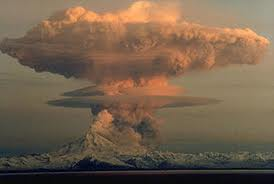
\includegraphics[width=.90\textwidth]{./PPT/Plume_pic}
\end{minipage}
\begin{minipage}{.49\textwidth}
\center
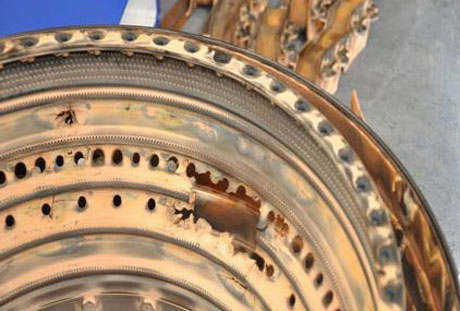
\includegraphics[width=.70\textwidth]{./PPT/BA-engine}
\end{minipage}
\\
\begin{minipage}{.32\textwidth}
\center
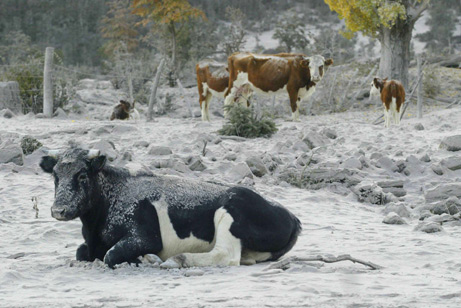
\includegraphics[width=.95\textwidth]{./PPT/Ash_community}
\end{minipage}
\begin{minipage}{.32\textwidth}
\center
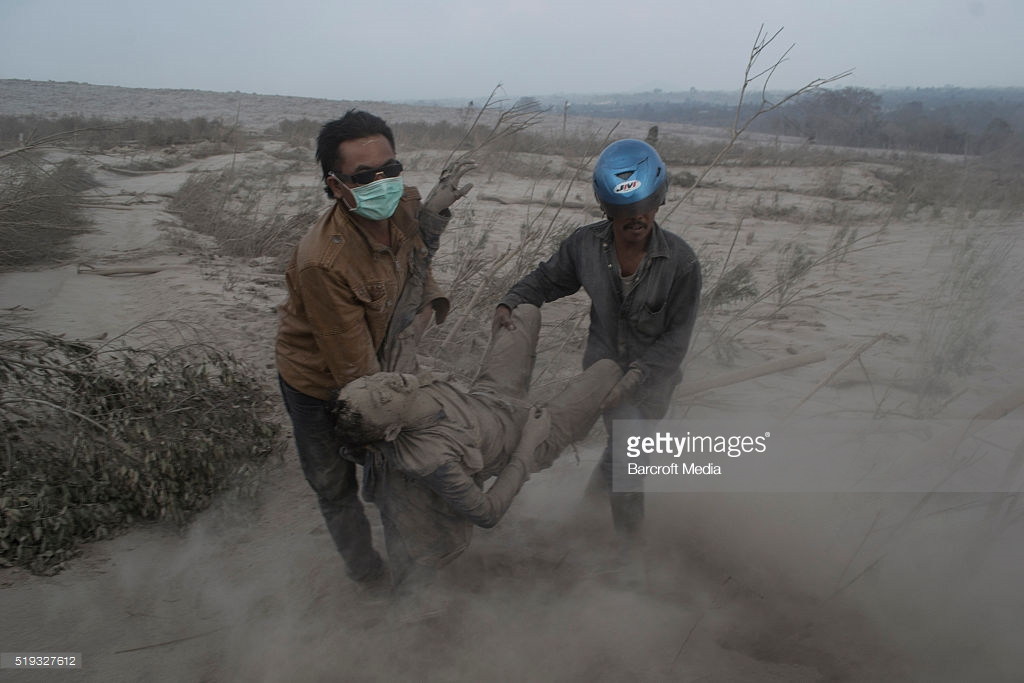
\includegraphics[width=.95\textwidth]{./PPT/Ash_community4}
\end{minipage}
\begin{minipage}{.32\textwidth}
\center
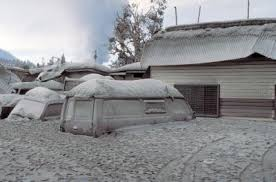
\includegraphics[width=.95\textwidth]{./PPT/Ash_community3}
\end{minipage}
\end{figure}

\begin{block} {Numerical tools}
\textbf{Four} 3D plumes models, around \textbf{Ten} 1D plume models, several VATDs.
\end{block}
\end{frame}

\begin{frame}{Motivation (Why a new model based on SPH)}
\begin{itemize}
%\item 3D plume model, less assumption, better predict capability
\item All existing 3D plume models are based on mesh-based method
\item And more importantly ...
\end{itemize}

\begin{figure}
\centering
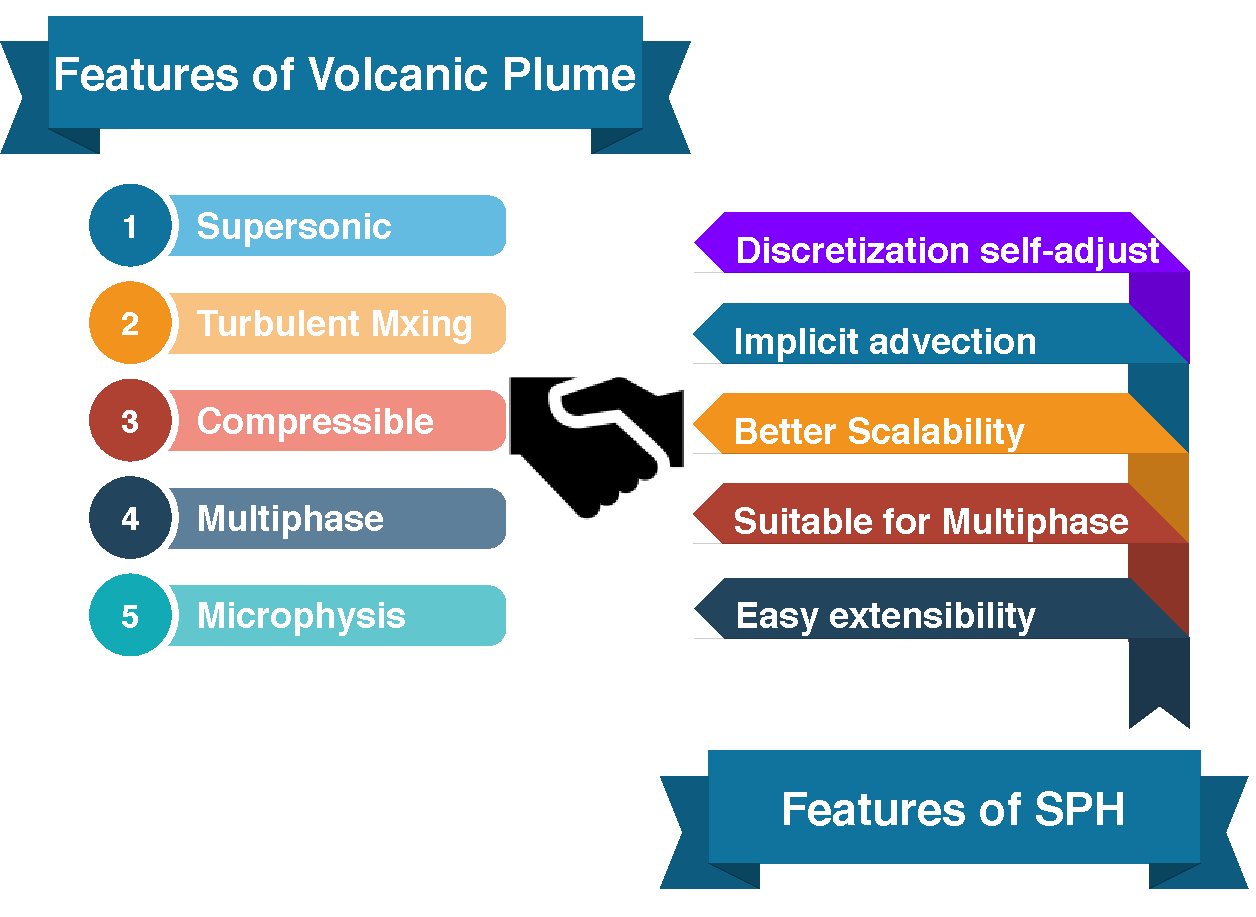
\includegraphics[width=.75\textwidth]{./PPT/Why_SPH}
\end{figure}
\end{frame}

\begin{frame}{Challenges}
\noindent
\begin{figure}
\centering
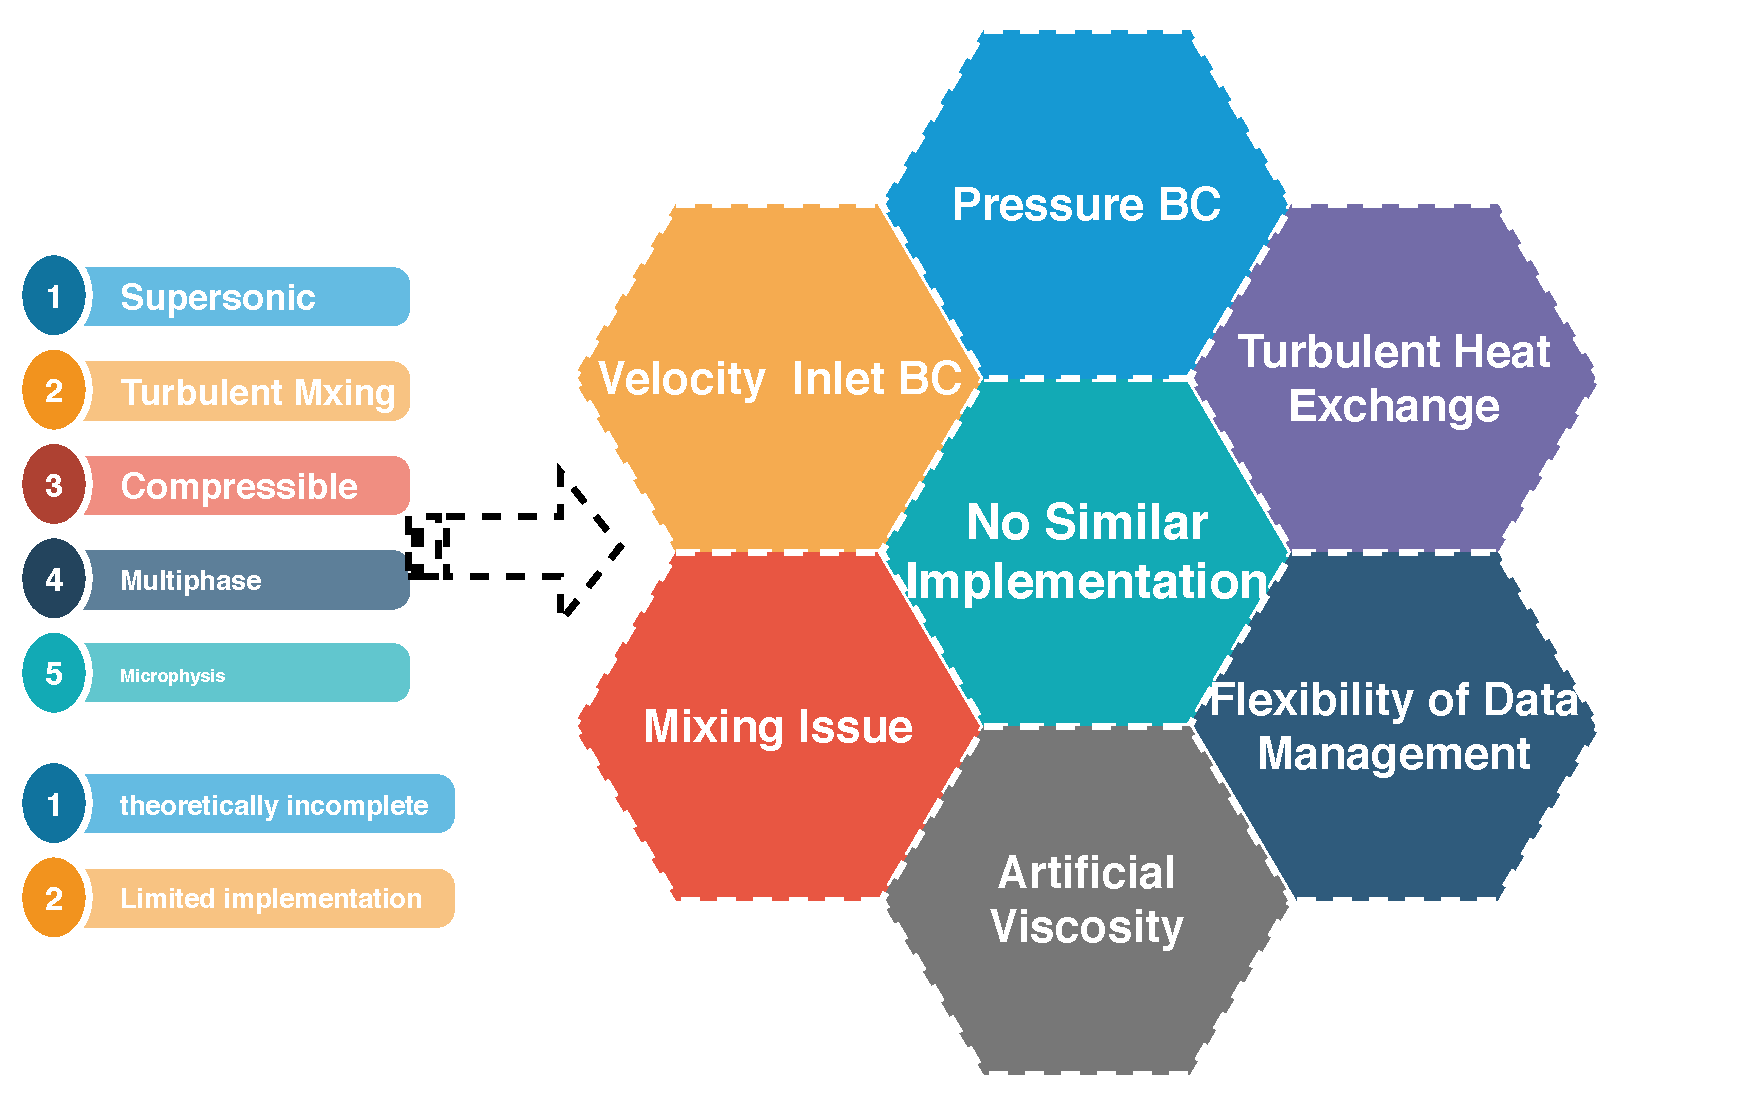
\includegraphics[width=.95\textwidth]{./PPT/Challenges}
\end{figure}
\end{frame}

%---------------------------------------------------------------------------
\section{Physics Model}

\begin{frame}{Governing Equations}
The governing equations\footcite{suzuki2005numerical}:\\
\begin{minipage}{.505\textwidth}
\begin{equation}
\dfrac{\partial \rho}{\partial t} + \nabla \cdot \left(\rho \textbf{v}\right) = 0 \label{eq:gov-cs-rho}
\end{equation}
\begin{equation}
\dfrac{\partial \rho \xi}{\partial t} + \nabla \cdot \left(\rho \xi \textbf{v}\right) = 0 \label{eq:gov-cs-ks}
\end{equation}
\begin{equation}
\dfrac{\partial \rho \textbf{v}}{\partial t} + \nabla \cdot \left(\rho \textbf{v} \textbf{v} + p\textbf{I}\right) = \rho \textbf{g} \label{eq:gov-cs-v} \\
\end{equation}
\begin{equation}
\dfrac{\partial \rho E}{\partial t} + \nabla \cdot \left[\left(\rho E + p \right)\textbf{v}\right] = \rho \textbf{g} \cdot\textbf{v} \label{eq:gov-cs-e}
\end{equation}\\
EOS for closing the system of equations
\begin{equation}
p = \left(\gamma_m - 1\right)\rho e \label{eq:EOS}
\end{equation}
%
\end{minipage} % This must go next to `\end{minipage}`
%
\begin{minipage}{.01\textwidth}
$\vert$\\
$\vert$\\
$\vert$\\
$\vert$\\
$\vert$\\
$\vert$\\
$\vert$\\
$\vert$\\
$\vert$\\
$\vert$\\
\end{minipage}
\begin{minipage}{.46\textwidth}
Specific heat ratio $\gamma_m$ is updated based on massfraction of erupted material:
\begin{equation}
\gamma_m = R_m/C_{vm} + 1 \label{eq:gov-gm}
\end{equation}
\begin{equation}
R_m = \xi_g R_g + \xi_a R_a  \label{eq:gov-Rm}
\end{equation}
\begin{equation}
C_{vm} = \xi_s C_{vs} + \xi_g C_{vg} + \xi_a C_{va} \label{eq:gov-Cvm}
\end{equation}
\begin{equation}
\xi_a = 1 - \xi \label{eq:gov-na}
\end{equation}
\begin{equation}
\xi_g = \xi \cdot \xi_{g0} \label{eq:gov-ng}
\end{equation}
\begin{equation}
\xi_s = \xi - \xi_g \label{eq:gov-ns}
\end{equation}
\end{minipage}
%
\end{frame}
%
\begin{frame}{Boundary Conditions}
\noindent
\begin{minipage}{.41\textwidth}
\textbf{Eruption BC}
\begin{align}
\rho =const = p/\left(R_m T\right) \label{eq:erupt_bc_rho} \\
\xi=const=1 \label{eq:erupt_bc_xi}\\
\textbf{v} = const =\{u,v,w\}^T \label{eq:erupt_bc_v}\\
\dfrac{\partial e}{\partial n}=\dot M e /\left(\pi r^2\right) \label{eq:erupt_bc_e}
\end{align} 
\textbf{No-slip wall BC}
\begin{align}
\dfrac{\partial \rho}{\partial n} = const = 0\label{eq:wall_bc_rho} \\
\dfrac{\partial \xi}{\partial n} = const = 0 \label{eq:wall_bc_xi}\\ 
\textbf{v} = const =\{0,0,0\}^T \label{eq:wall_bc_v}\\
\dfrac{\partial e }{\partial n} = 0\label{eq:wall_bc_e}
\end{align} 
\end{minipage} % This must go next to `\end{minipage}`
%
\begin{minipage}{.01\textwidth}
$\vert$\\
$\vert$\\
$\vert$\\
$\vert$\\
$\vert$\\
$\vert$\\
$\vert$\\
$\vert$\\
$\vert$\\
$\vert$\\
$\vert$\\
$\vert$\\
$\vert$\\
$\vert$\\
$\vert$\\
$\vert$\\
$\vert$\\
\end{minipage}
\begin{minipage}{.560\textwidth}
\begin{minipage}[!t]{\textwidth}
\textbf{Pressure outlet BC}
\begin{equation}
p = p_a\left(z\right)\label{eq:pressure_bc_p} 
\end{equation} 
\end{minipage}
%
\\[20mm]
%
\begin{minipage}{0.49\textwidth}
\begin{figure}[!t]
\centering
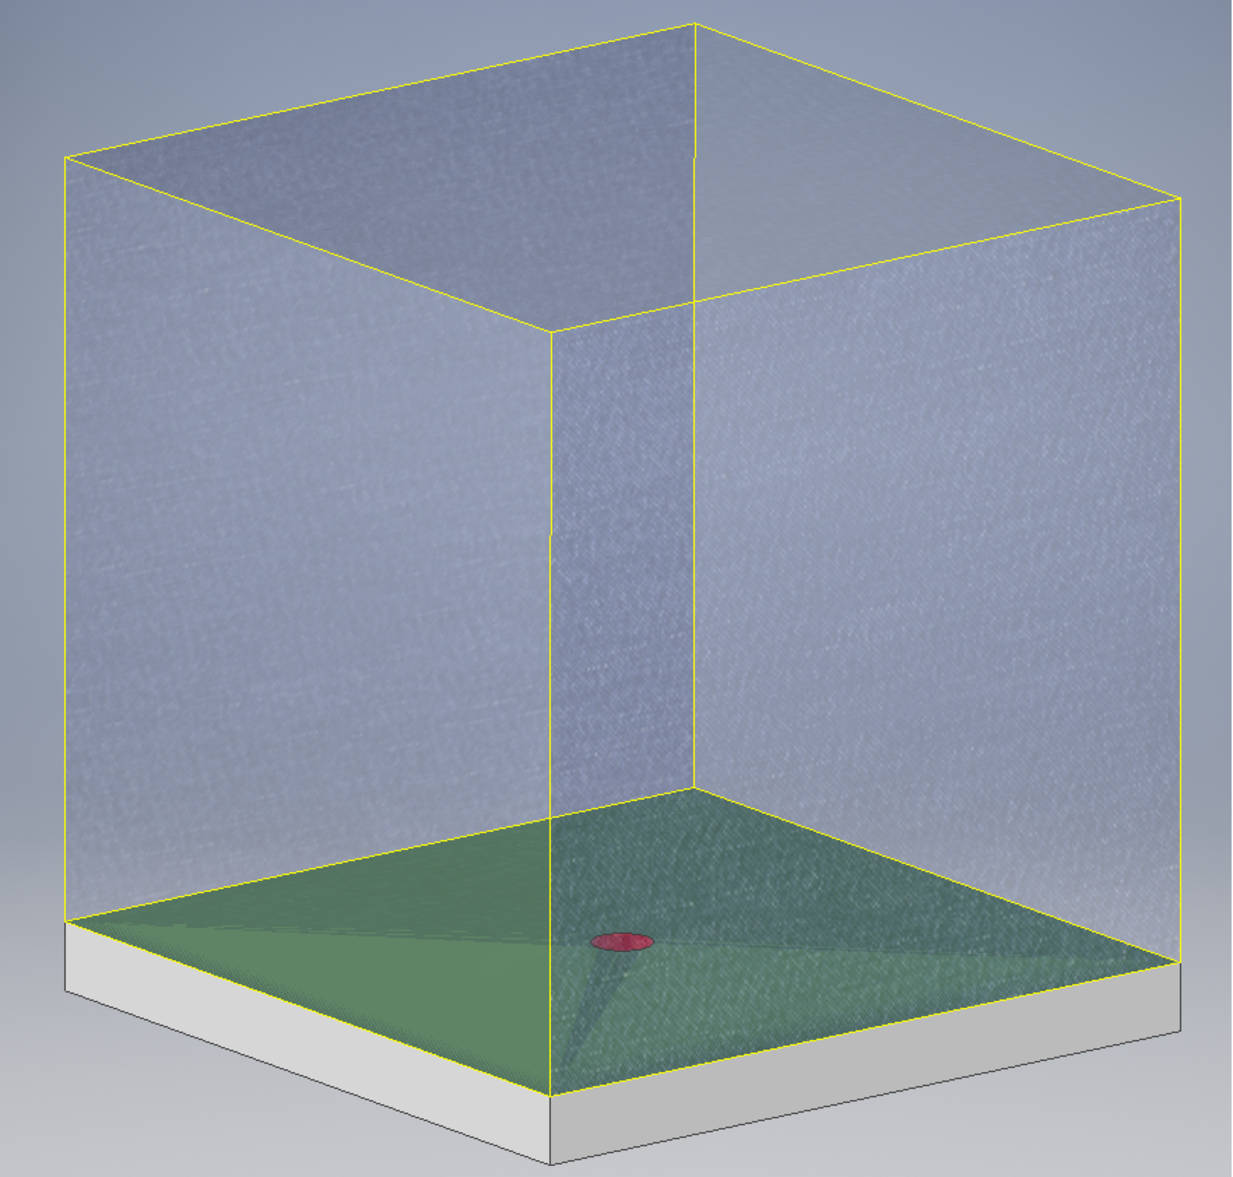
\includegraphics[width=.99\textwidth]{./Chapter-2/Figures/Domain_good}
%\caption{Scope of the problem}
\label{fig:Domain_3D}
\end{figure}
\end{minipage}
\begin{minipage}{0.49\textwidth}
\begin{figure}[!t]
\centering
\includegraphics[width=.99\textwidth]{./Chapter-5/Figures/Boundary-condition-eps-converted-to}
\end{figure}
\end{minipage}
%
\end{minipage}
%
\end{frame}

\begin{frame}{Eigenstructure}
\noindent
\begin{minipage}{.54\textwidth}
\begin{figure}
\centering
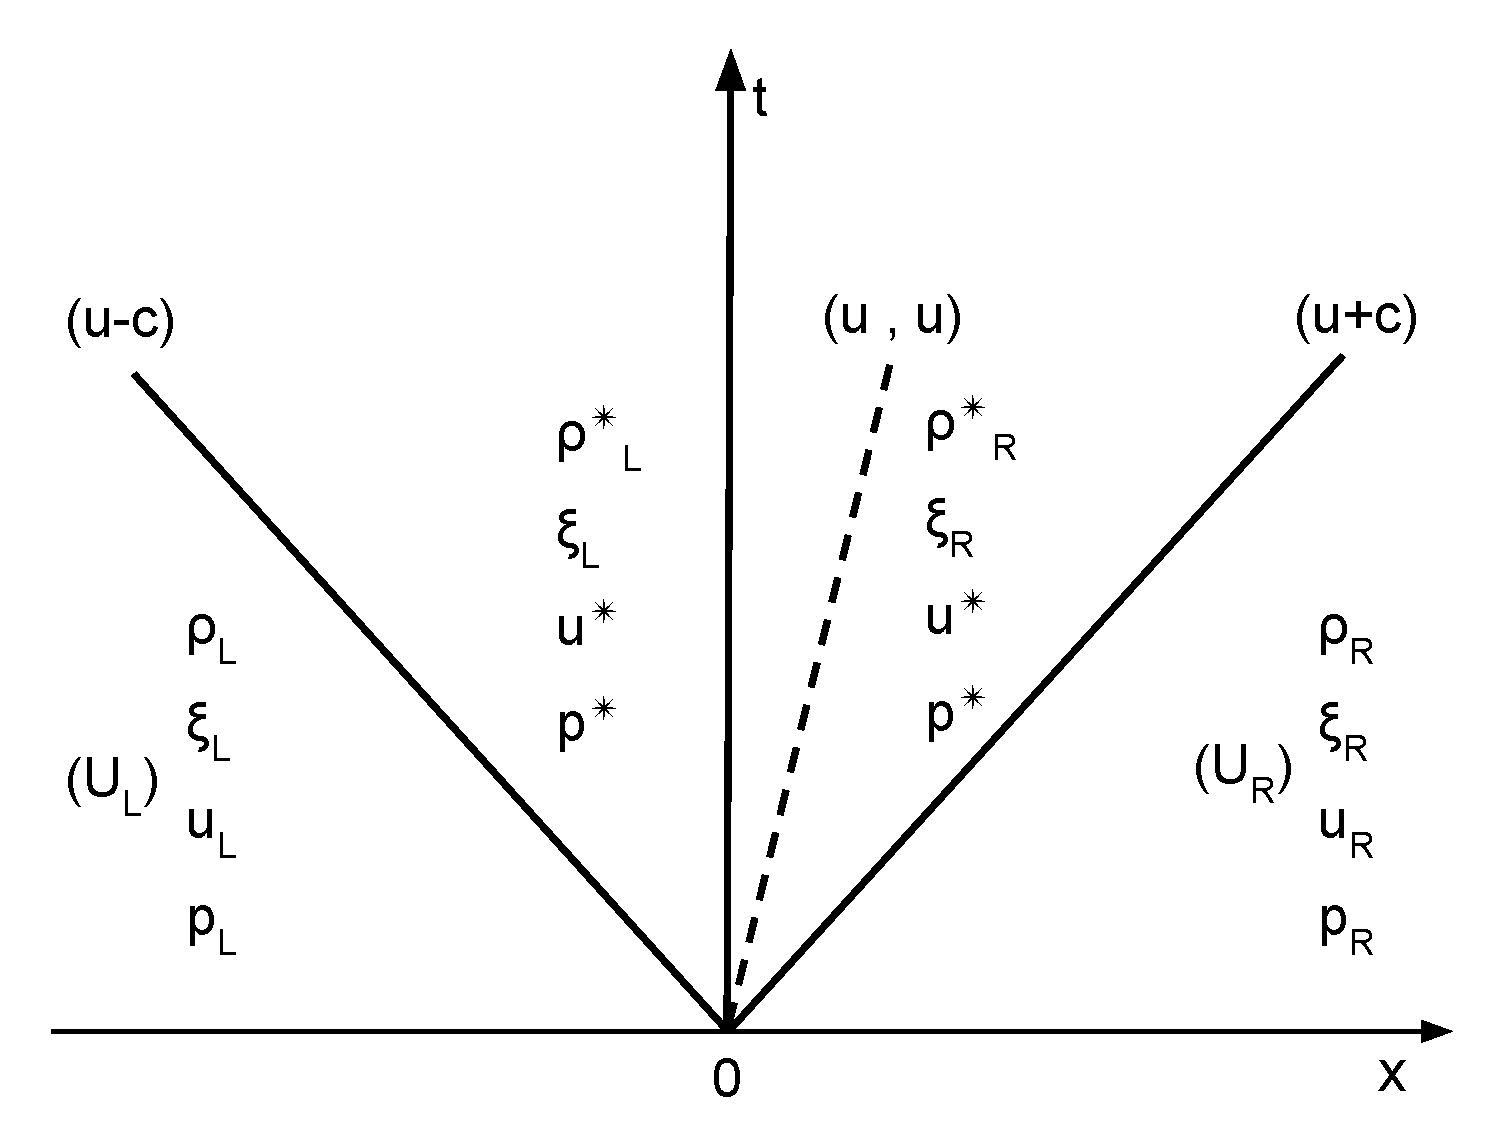
\includegraphics[width=.85\textwidth]{./Chapter-2/Figures/Solution_Structure_RP}
\label{fig:Domain_3D}
\end{figure}
\large{\textbf{Eignenstructure of Jacobian of Flux}}
\begin{itemize}
\item two nonlinear characteristic fields($u \pm c_m$), and two linear degenerate ($u$)
\end{itemize} 

\end{minipage}
\begin{minipage}{.01\textwidth}
$\vert$\\
$\vert$\\
$\vert$\\
$\vert$\\
$\vert$\\
$\vert$\\
$\vert$\\
$\vert$\\
$\vert$\\
$\vert$\\
$\vert$\\
$\vert$\\
$\vert$\\
$\vert$\\
$\vert$\\
$\vert$\\
$\vert$\\
\end{minipage}
\begin{minipage}{.43\textwidth}
\begin{itemize}
\item only $\rho$ changes accross second wave, only $\xi$ changes accross the third wave.
\item \textbf{$\xi$ keeps constant accross shocks}
\item \textbf{$\xi$ keeps constant accross rarefactions}
\item $c_m$, $\gamma_m$ depends on $\xi$.
\end{itemize} 
\begin{figure}
\centering
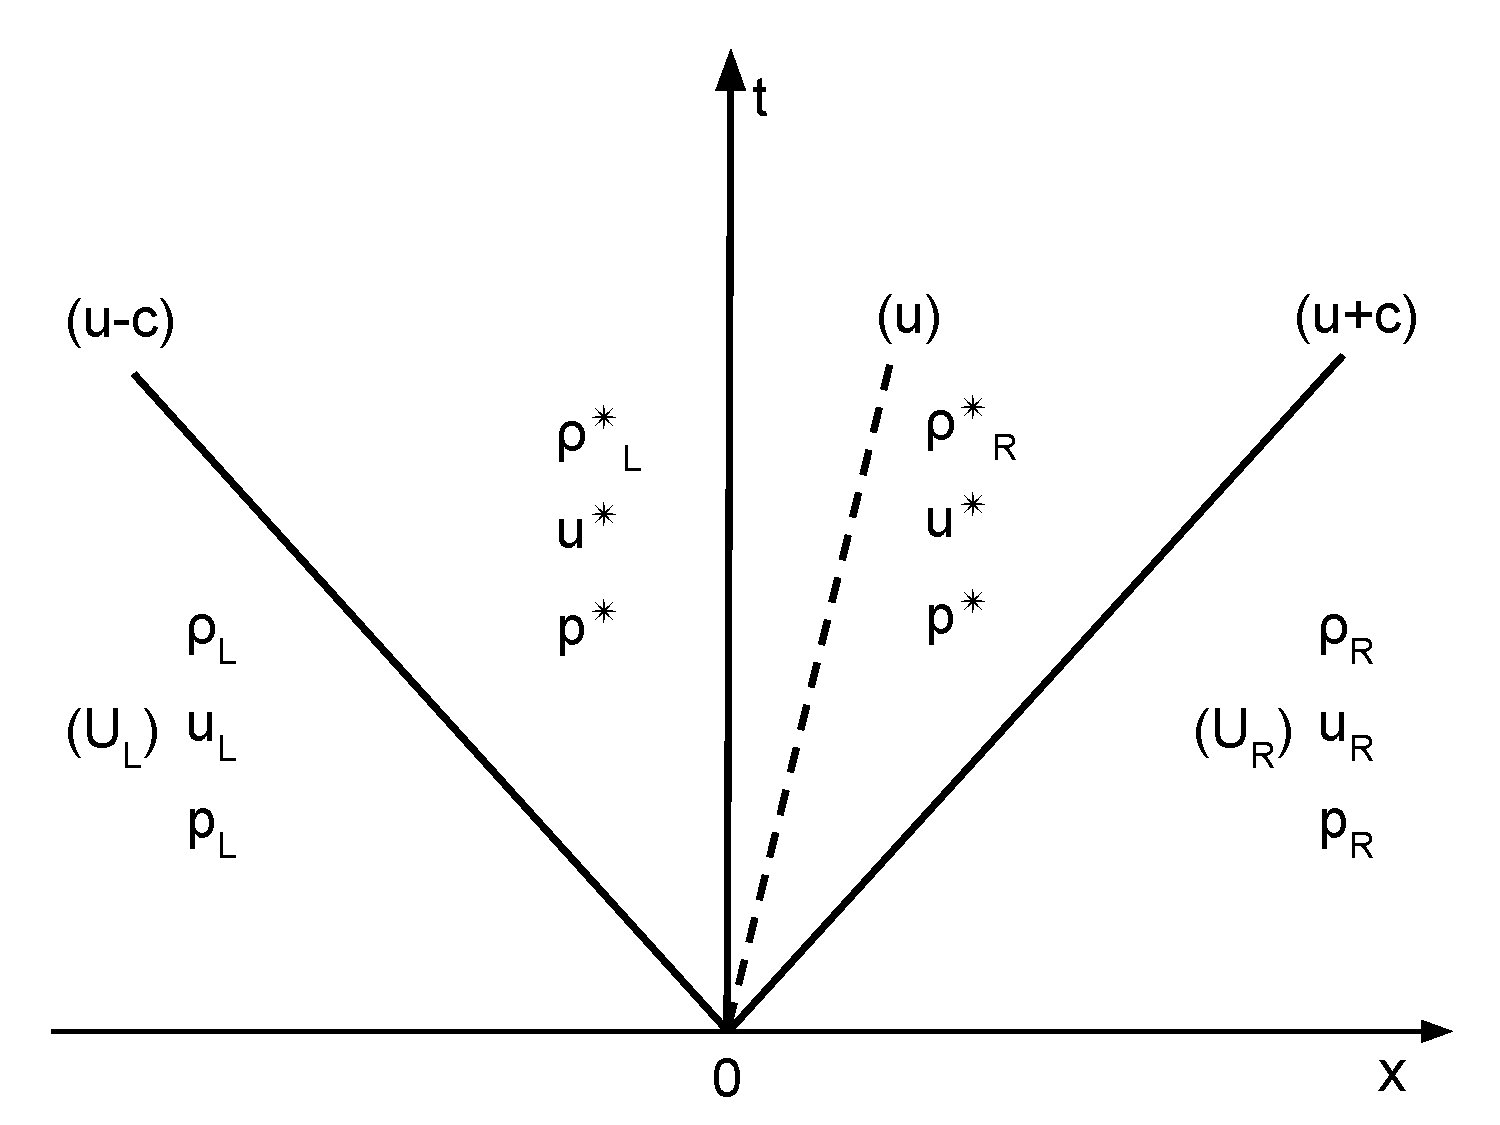
\includegraphics[width=.80\textwidth]{./Chapter-2/Figures/Solution_Structure_RP_simplified}
\label{fig:Domain_3D}
\end{figure}
\end{minipage}
%
\end{frame}

\section{SPH Discretization}
\begin{frame}{SPH Basic}
\noindent
\begin{minipage}{0.63 \textwidth}
Approximation of function $A$ and its derivative:
\begin{equation}
<A\left(\textbf{x}\right)> \approx \sum_b m_b \dfrac{A_b}{\rho_b} w\left(\textbf{x}-\textbf{x}_b, h\right)
\label{eq:SPH-approximation-sum}
\end{equation}
\begin{equation}
\begin{split}
<\nabla A\left(\textbf{x}\right)> \approx \sum_b m_b \dfrac{A_b}{\rho_b} \nabla w\left(\textbf{x} - \textbf{x}_b, h\right)
\end{split} 
\label{eq:SPH-scalar-function-gradient}
\end{equation}
\end{minipage}
\begin{minipage}{0.36 \textwidth}
\begin{figure}
\center
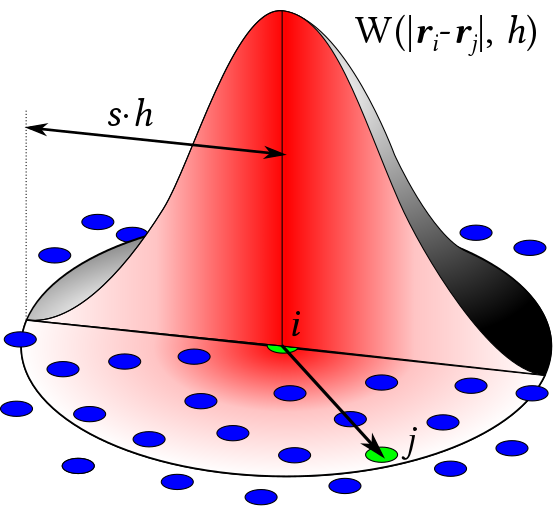
\includegraphics[width=0.99\textwidth]{./PPT/SPH-interpolation}
\end{figure}
\end{minipage}

Truncated Guassian kernel functions
\begin{equation}
w\left(\textbf{x} - \textbf{x}_b\right) = 
\begin{cases} 
      \dfrac{1}{\left(h \sqrt{\pi}\right)^d} exp \left[- \left(\dfrac{\textbf{x} - \textbf{x} \prime}{h} \right)^2 \right] &  \vert \textbf{x} - \textbf{x} \prime \vert \leq 3h\\
      0 & \text{Otherwise}
\end{cases}
\label{eq:SPH-kernel}
\end{equation}
\end{frame}

\begin{frame}{SPH Basic-Example (Euler euqation) }
\begin{align}
<\rho_a> = \sum_b m_b w_{ab} \left(h\right) \label{eq:ns-sph-d} \\
\left\langle\dfrac{d \textbf{v}_a}{d t}\right\rangle = -\sum_b m_b \left(\dfrac{p_b}{\rho_b^2} + \dfrac{p_a}{\rho_a^2} + \Pi_{ab}\right) \nabla_a w_{a b}\left(h\right) +\textbf{g} \label{eq:ns-sph-v} \\
\left\langle\dfrac{d e_a}{d t}\right\rangle=
 0.5\sum_b m_b \textbf{v}_{a b}\left(\dfrac{p_b}{\rho_b^2} + \dfrac{p_a}{\rho_a^2} + \Pi_{ab}\right) \cdot \nabla_a w_{a b}\left(h\right) \label{eq:ns-sph-e}
\end{align}
$\textbf{v}_{a b} = \textbf{v}_a - \textbf{v}_b$. $\Pi$ is an artificial viscosity term
\begin{equation}
\Delta t = \textrm{CFL} \min_a \bigg \lbrace \dfrac{\left[\frac{m_a}{\rho_a}\right]^{\frac{1}{d}}}{c_a} \bigg \rbrace
\end{equation}
Particle position is also updated at every time step.
\begin{equation}
\left\langle\dfrac{d \textbf{x}_a}{dt}\right\rangle = \textbf{v}_a \label{eq:SPH-update-pos}
\end{equation}
\end{frame}

\begin{frame}{Tensile Instability and Corrected Derivatives}
To handle tensile instability and boundary deficiency, adopt a corrected SPH formulation \footcite{chen1999improvement}.
\begin{equation}
\begin{split}
\int_{\Omega} A\left(x\right) w\left(x- x_a, h\right) dx &= 
A_a \int_{\Omega} w\left(x - x_a, h\right) dx \\  & +A_{xa} \int_{\Omega} \left(x-x_a\right) w\left(x - x_a, h\right) dx +...
\end{split}
\end{equation}
\\
\noindent
\begin{minipage}{0.99 \textwidth}
\begin{minipage}{0.60 \textwidth}
\begin{equation}
A_a = \frac{\sum_b m_b \dfrac{A_b}{\rho_b} w\left(x_a-x_b, h\right)}{\sum_b m_b \dfrac{1}{\rho_b} w\left(x_a-x_b, h\right)}
\label{eq:CSP-function-approximation-1d}
\end{equation}
\begin{equation}
\nabla A_a = \frac{\sum_b m_b \dfrac{A_b - A_a}{\rho_b} \nabla_a w\left(x_a-x_b, h\right)}{\sum_b m_b \dfrac{x_b - x_a}{\rho_b} \nabla_a w\left(x_a-x_b, h\right)}
\end{equation}
\end{minipage}
\begin{minipage}{.01\textwidth}
$\vert$\\
$\vert$\\
$\vert$\\
$\vert$\\
$\vert$\\
$\vert$\\
$\vert$\\
$\vert$\\
$\vert$\\
\end{minipage}
\begin{minipage}{0.37 \textwidth}
\begin{equation}
\int	 w\left(\textbf{x}-\textbf{x}\prime, h\right) d\textbf{x}\prime = 1
\label{eq:SPH-kernel-normalization-prop}
\end{equation}
\begin{equation}
\sum_b m_b \dfrac{x_b - x_a}{\rho_b} \nabla w_{ab} = 1 
\label{eq:SPH-kernel-normalization-prop}
\end{equation}
\end{minipage}
%
\end{minipage}
%
\end{frame}

\begin{frame}{Interface Construction}
\noindent
\begin{minipage}{0.65 \textwidth}
In our model, only density needs to be updated respectively for each phase:
\begin{equation}
<\rho_{\alpha}^a>=\frac{\sum m_b w_{\alpha b} \left(h\right)}{\sum \frac{m_b}{\rho_b} w_{\alpha b} \left(h\right) +\sum \frac{m_j}{\rho_j} w_{\alpha j} \left(h\right)} \label{eq:gov-sph-d1}
\end{equation}
\begin{equation}
<\rho_\alpha^{sg}>=\frac{\sum_j m_j w_{\alpha j} \left(h\right)}{\sum \frac{m_b}{\rho_b} w_{\alpha b} \left(h\right) +\sum \frac{m_j}{\rho_j} w_{\alpha j} \left(h\right)} \label{eq:gov-sph-d2}
\end{equation}
\begin{equation}
<\xi_{\alpha}> = \dfrac{\rho^{sg}_{\alpha}}{\rho_{\alpha}^{a}+\rho_{\alpha}^{sg}}
\label{eq:gov-sph-xi}
\end{equation}
\end{minipage}
\begin{minipage}{0.27 \textwidth}
\begin{figure}
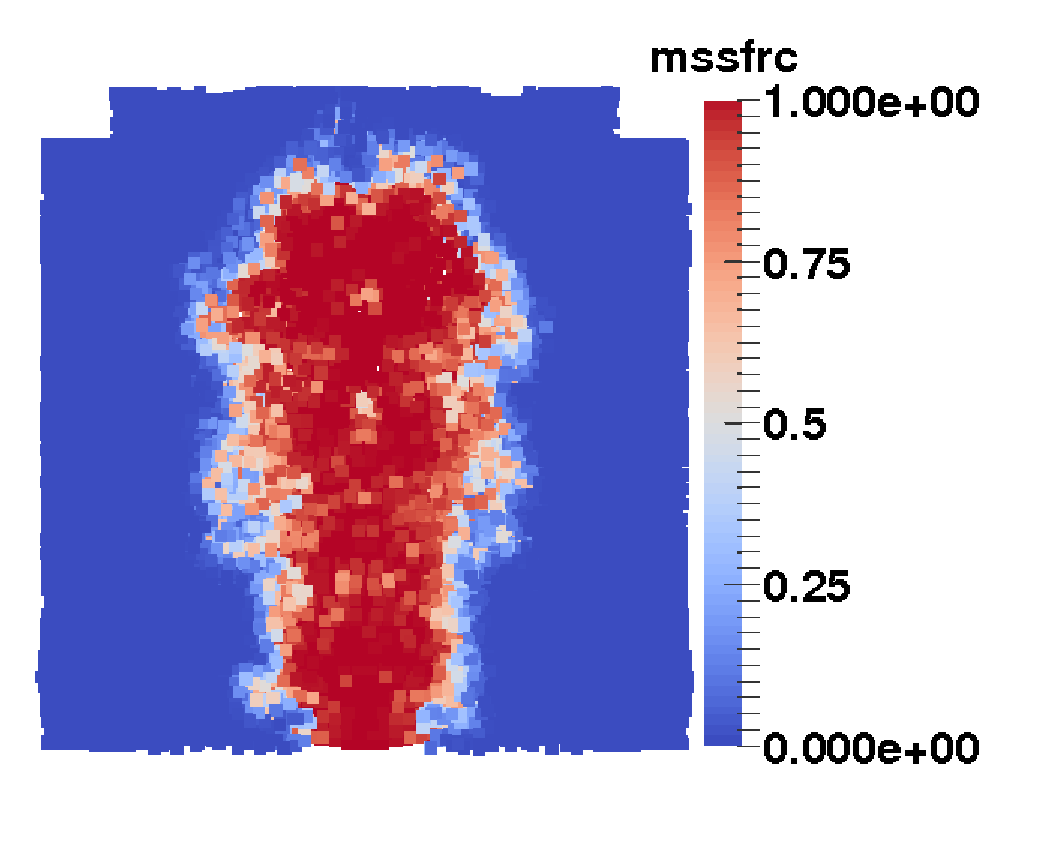
\includegraphics[width=0.95 \textwidth]{./PPT/Interface_msf_rs}
\end{figure}
\begin{figure}
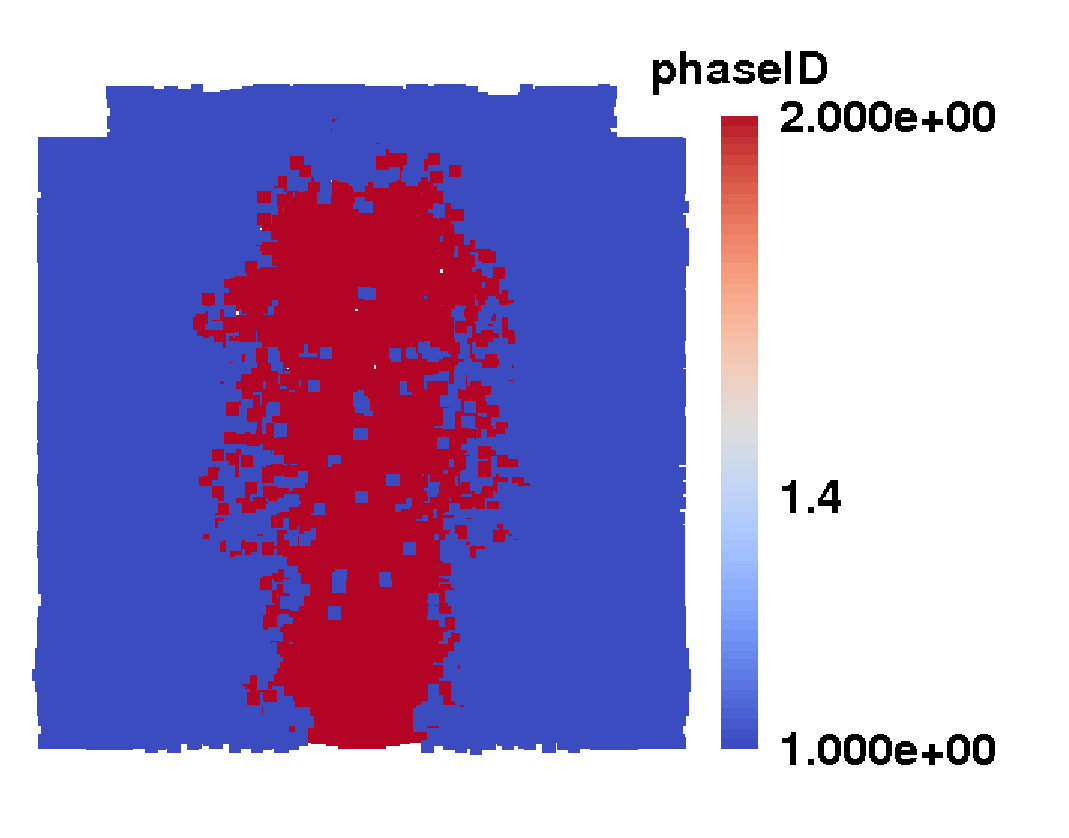
\includegraphics[width=0.95 \textwidth]{./PPT/Interface_phase_rs}
\end{figure}
\end{minipage}

\begin{block}{}
  \begin{itemize}
    \item {The mass discontinuity and density discontinuity issues in traditional formulations of SPH is fixed by this new formulation
    } 
    \item {In areas far away from the interface, updating of density is exactly the same as that for single phase flow
    }
 \end{itemize}
\end{block}
\end{frame}

\begin{frame}{A LANS Type Turbulence Model}
To capture sub-particle scale momentum and energy exchange due to turbulence, we adopt a LANS type turbulence model \footcite{monaghan2011turbulence}.\\
\noindent
\begin{minipage}{0.65 \textwidth}
Velocity is filtered (averaged) in space
\begin{equation}
\widehat{\textbf{v}}\left(\textbf{x}\right)=\textbf{v}\left(\textbf{x}\right)+ \epsilon \int \left(\textbf{v}\left(\textbf{x} \prime\right)-\textbf{v}\left(\textbf{x}\right)\right)G\left(\vert \textbf{x} \prime - \textbf{x} \vert, l\right) d\textbf{x} \prime
\end{equation}
Where $G$ satisfies:
\begin{equation}
\int G\left(\vert \textbf{x} \prime - \textbf{x} \vert, l\right) d\textbf{x} \prime =1
\end{equation}
\begin{equation}
\lim _{l \rightarrow 0} G\left(\textbf{x} \prime-\textbf{x}, l\right) =  \delta \left(\textbf{x} \prime - \textbf{x}\right)
\label{eq:SPH_kernel_delta}
\end{equation}
Introduces an extra turbulence stress term:
\begin{equation}
\Phi_{ab}=\dfrac{\varepsilon}{2} \dfrac{\textbf{v}_{ab} \cdot \textbf{v}_{ab}}{\rho_b} \label{eq:_LANS_trub_stress}
\end{equation}
\end{minipage}
%
\begin{minipage}{0.34 \textwidth}
\begin{figure}
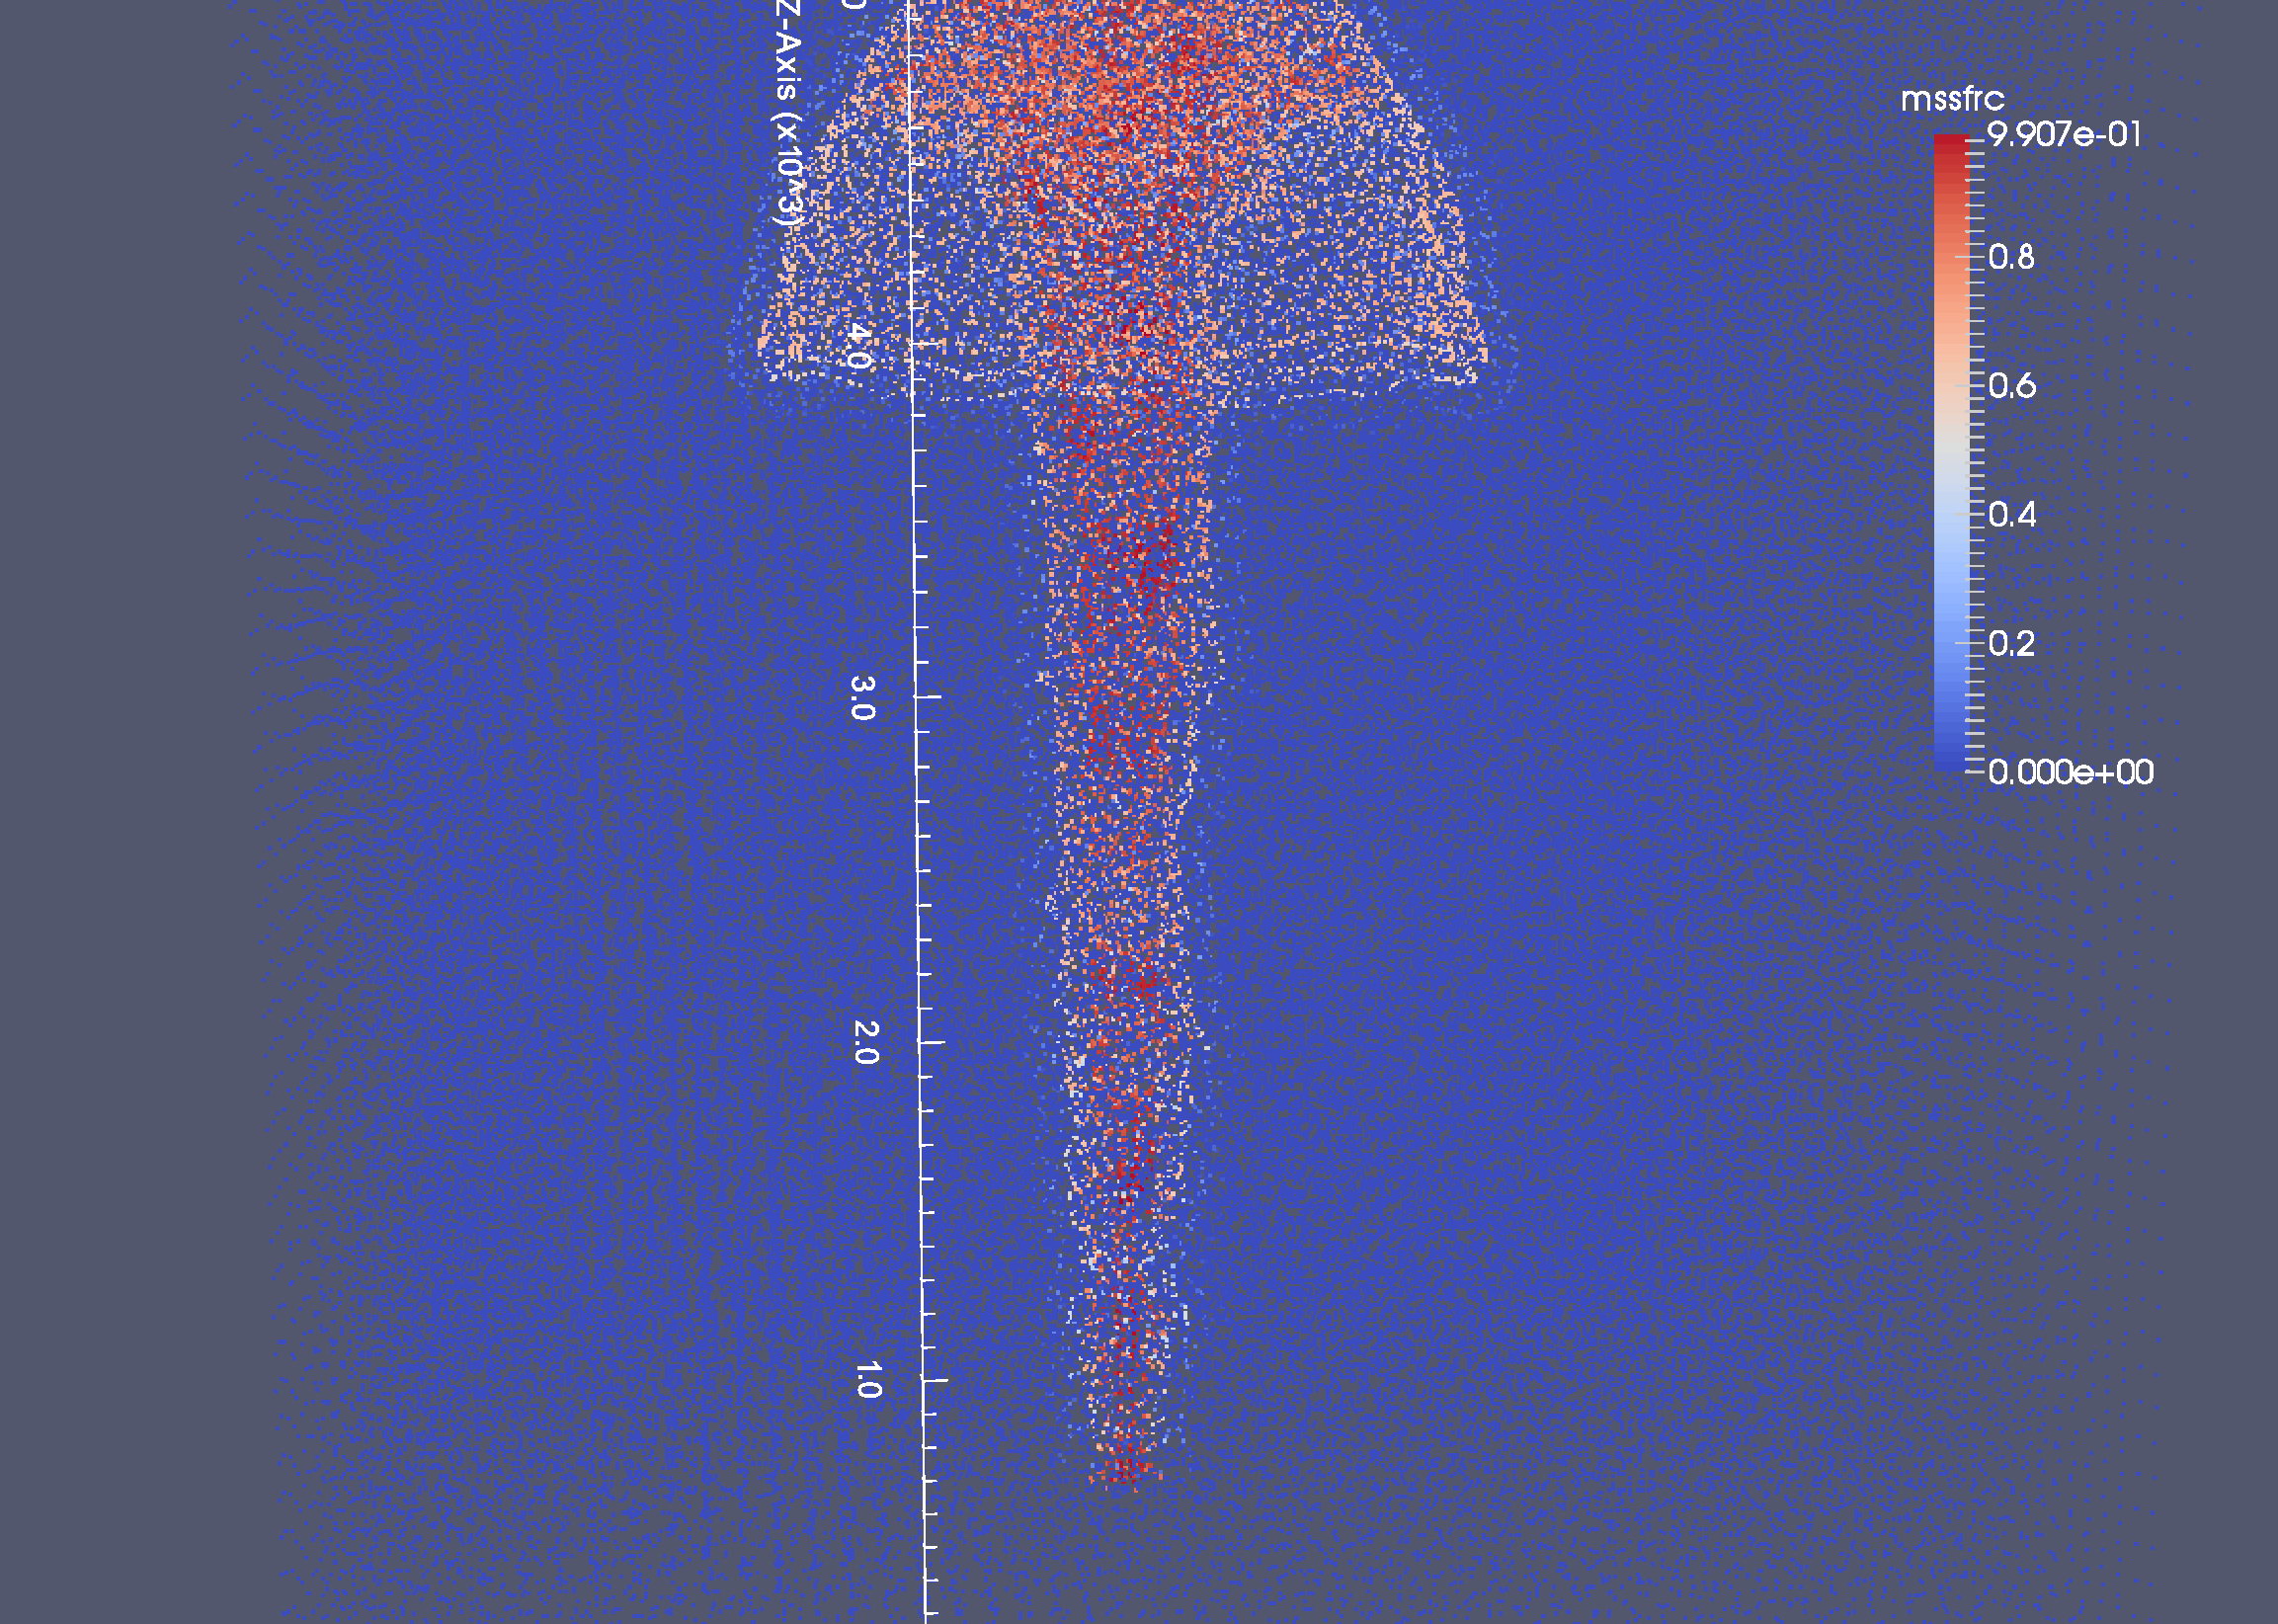
\includegraphics[width=0.80 \textwidth]{./PPT/No_turb}
\end{figure}
%
\begin{figure}
\includegraphics[width=0.80 \textwidth]{./Chapter-6/Figures/JPUE_entrainment}
\end{figure}
\end{minipage}
\end{frame}

\begin{frame}{Turbulent Energy Exhange}
Use Reynolds analogy to model the heat transfer due to turbulence \footcite{gmd-2017-119}.
\begin{equation}
Pr=\dfrac{C_p \mu}{\kappa}
\end{equation}
The ratio between turbulent shear stress and physical shear stress is calculated for each pair of particles:
\begin{equation}
\begin{split}
\Upsilon_{ab} &= \dfrac{\dfrac{\varepsilon}{2} \dfrac{\textbf{v}_{ab} \cdot \textbf{v}_{ab}}{\rho_b}}{\dfrac{S \nu}{\rho_{ab}} \frac{\textbf{v}_{ab} \cdot \textbf{x}_{ab}}{x_{ab}^2 + \eta^2 h_{ab}^2}} \\
 & = \dfrac{\varepsilon \left(x_{ab}^2 + \eta^2 h_{ab}^2\right)}{2 S \nu} \dfrac{\textbf{v}_{ab} \cdot \textbf{v}_{ab}}{\textbf{v}_{ab} \cdot \textbf{x}_{ab}}
\end{split}
\end{equation}
\begin{equation}
\kappa_{t,ab}= 
\begin{cases} 
      0 & if \quad \textbf{v}_{ab} \cdot \textbf{x}_{ab} = 0 \\
      \dfrac{\varepsilon \bar{C}_{p,ab} \bar{\rho}_{ab} x_{ab}^2 \textbf{v}_{ab} \cdot \textbf{v}_{ab}}{2 S Pr_t \bar{h}_{ab} \bar{c}_{ab} \textbf{v}_{ab} \cdot \textbf{x}_{ab} } & \text{otherwise}
\end{cases}
\label{eq:SPH-LANS-heat-conductivity}
\end{equation}
\end{frame}

\begin{frame}{Numerical dissipation}
Classicial SPH includes artificial viscosity explicitly to 
\begin{itemize}
\item stabilizing the simulation 
\item handling shock discontinuities in supersonic flow
\end{itemize}
\begin{equation}
\Pi_{ab}^{\beta} = 
\begin{cases} 
      \dfrac{- \alpha \mu_{ab} \bar{c}_{ab} + \beta \mu_{ab}^2} {\bar{\rho}_{ab}} & \textbf{v}_{ab} \cdot \textbf{x}_{ab} < 0\\
      0 & \textbf{v}_{ab} \cdot \textbf{x}_{ab} > 0
\end{cases}
\label{eq:art-vis-shock}
\end{equation}
Where
\begin{equation}
\mu_{ab} = \dfrac{h \textbf{v}_{ab} \cdot \textbf{x}_{ab}}{\textbf{x}_{ab}^2 + \left(\eta h\right)^2} 
\end{equation}

However, the artificial dissipation introduced in this way usually is more than needed resulting in undesirable smearing of discontinuity and overwhelms fluid turbulence.
\end{frame}

\begin{frame}{RSPH and GSPH}
Discretized formulation of RSPH is exactly the same as that of GSPH \footcite{inutsuka2002reformulation}.
\begin{equation}
\ddot{\textbf{x}}_{a} = <\dfrac{d \textbf{v}_{a}}{dt}>= -\sum_{b} m_{b} p_{a b}^{\ast} \left[\frac{1}{\rho_{a}^2} \nabla w_{a b}(h_{a}) + \frac{1}{\rho_{b}^2} \nabla w_{a b}(h_{b}) \right]
\label{eq:gov-gsph-v-simple-form}
\end{equation}
\begin{equation}
<\dfrac{d e_{a}}{dt}>= - \sum_{b} m_{b} p_{a b}^{\ast} [\textbf{v}_{a b}^{\ast} - \dot{\textbf{x}}_{a}^{\ast}] \left[\frac{1}{\rho_{a}^2} \nabla w_{a b}(h_{a}) + \frac{1}{\rho_{b}^2} \nabla w_{a b}(h_{b}) \right]
\label{eq:gov-gsph-e-simple-form}
\end{equation}
$\dot{\textbf{x}}_{a}^{\ast}$ is time centered velocity of particle $a$:
\begin{equation}
\dot{\textbf{x}}_{a}^{\ast} = <\textbf{v}_{a}> + \frac{\Delta t}{2} \ddot{\textbf{x}}_{a}
\label{eq:gsph-time-centered-velocity}
\end{equation}
Recall the classical SPH discretization
\begin{align}
\left\langle\dfrac{d \textbf{v}_a}{d t}\right\rangle = -\sum_b m_b \left(\dfrac{p_b}{\rho_b^2} + \dfrac{p_a}{\rho_a^2} + \Pi_{ab}\right) \nabla_a w_{a b}\left(h\right) +\textbf{g} \label{eq:ns-sph-v} \\
\left\langle\dfrac{d e_a}{d t}\right\rangle=
 0.5\sum_b m_b \textbf{v}_{a b}\left(\dfrac{p_b}{\rho_b^2} + \dfrac{p_a}{\rho_a^2} + \Pi_{ab}\right) \cdot \nabla_a w_{a b}\left(h\right) \label{eq:ns-sph-e}
\end{align}
\end{frame}

\begin{frame}{RSPH}
The basic procedure of RSPH\footcite{zhixuan2018rcm}\\
\begin{minipage}{0.45\textwidth}
\begin{itemize}
\item Establish a local coordinate system, project and define left and right states
\item Solve this local Riemann problem 
\item Sample the solution obtaining $p^{\ast}, u^{\ast}$ at $\theta \frac{|\textbf{x}_{a} - \textbf{x}_{ b}|}{2}$ relative to origin
\item Project $p^{\ast}, u^{\ast}$  back to the global coordinate system, get $p^{\ast}$ and $\textbf{v}^{\ast}$;
\item Update the particle positions and physical quantities.
\end{itemize}
\end{minipage}
\begin{minipage}{.54 \textwidth}
\begin{equation}
\hat{r}_{a b}= \frac{\textbf{x}_{a} - \textbf{x}_{ b}}{|\textbf{x}_{a} - \textbf{x}_{ b}|}
\end{equation}
\begin{equation}
u_{a}= \textbf{v}_{a} \cdot \hat{r}_{a b}
~~~~~~~~~~
u_{b}= \textbf{v}_{b} \cdot \hat{r}_{a b}
\label{eq:RP-project-2-local}
\end{equation}
\begin{figure}
    \center
	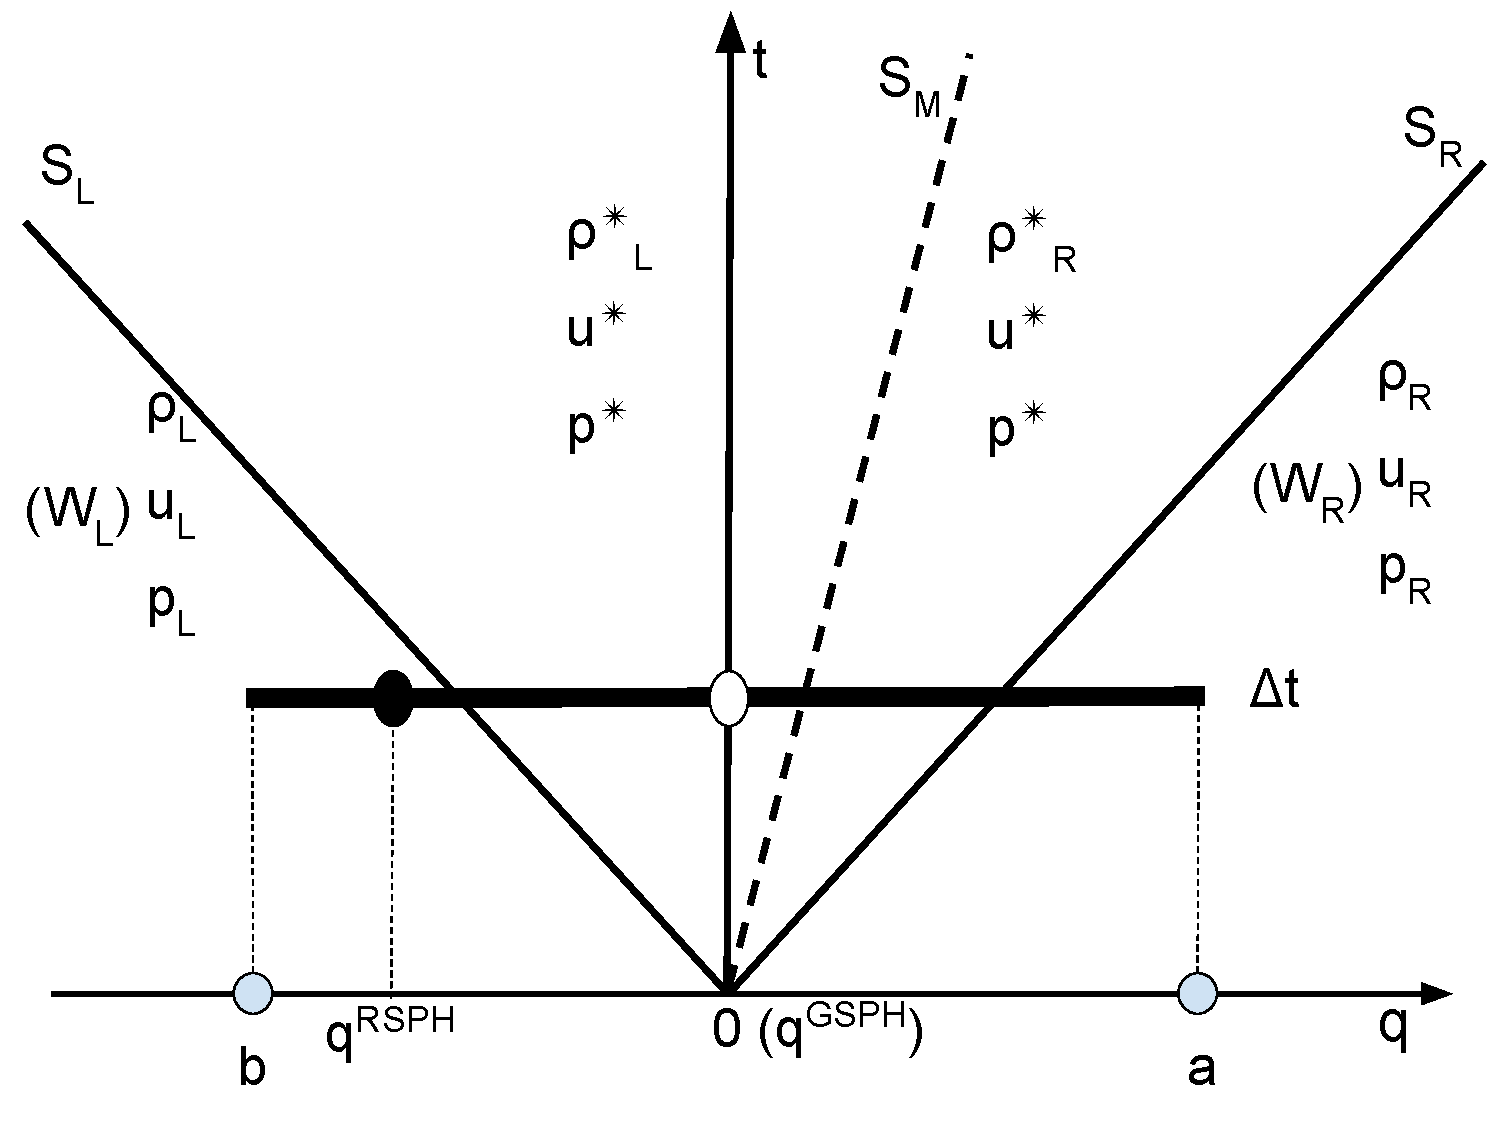
\includegraphics[width=0.85 \textwidth]{./Chapter-4/Figures/RSPH-GSPH}
    \label{fig:pick-up-state-GSPH-RSPH}
\end{figure}

\end{minipage}
\end{frame}
%
\begin{frame}{Benchmark Tests}
 \center{ 
    \begin{minipage}{.3\textwidth}
        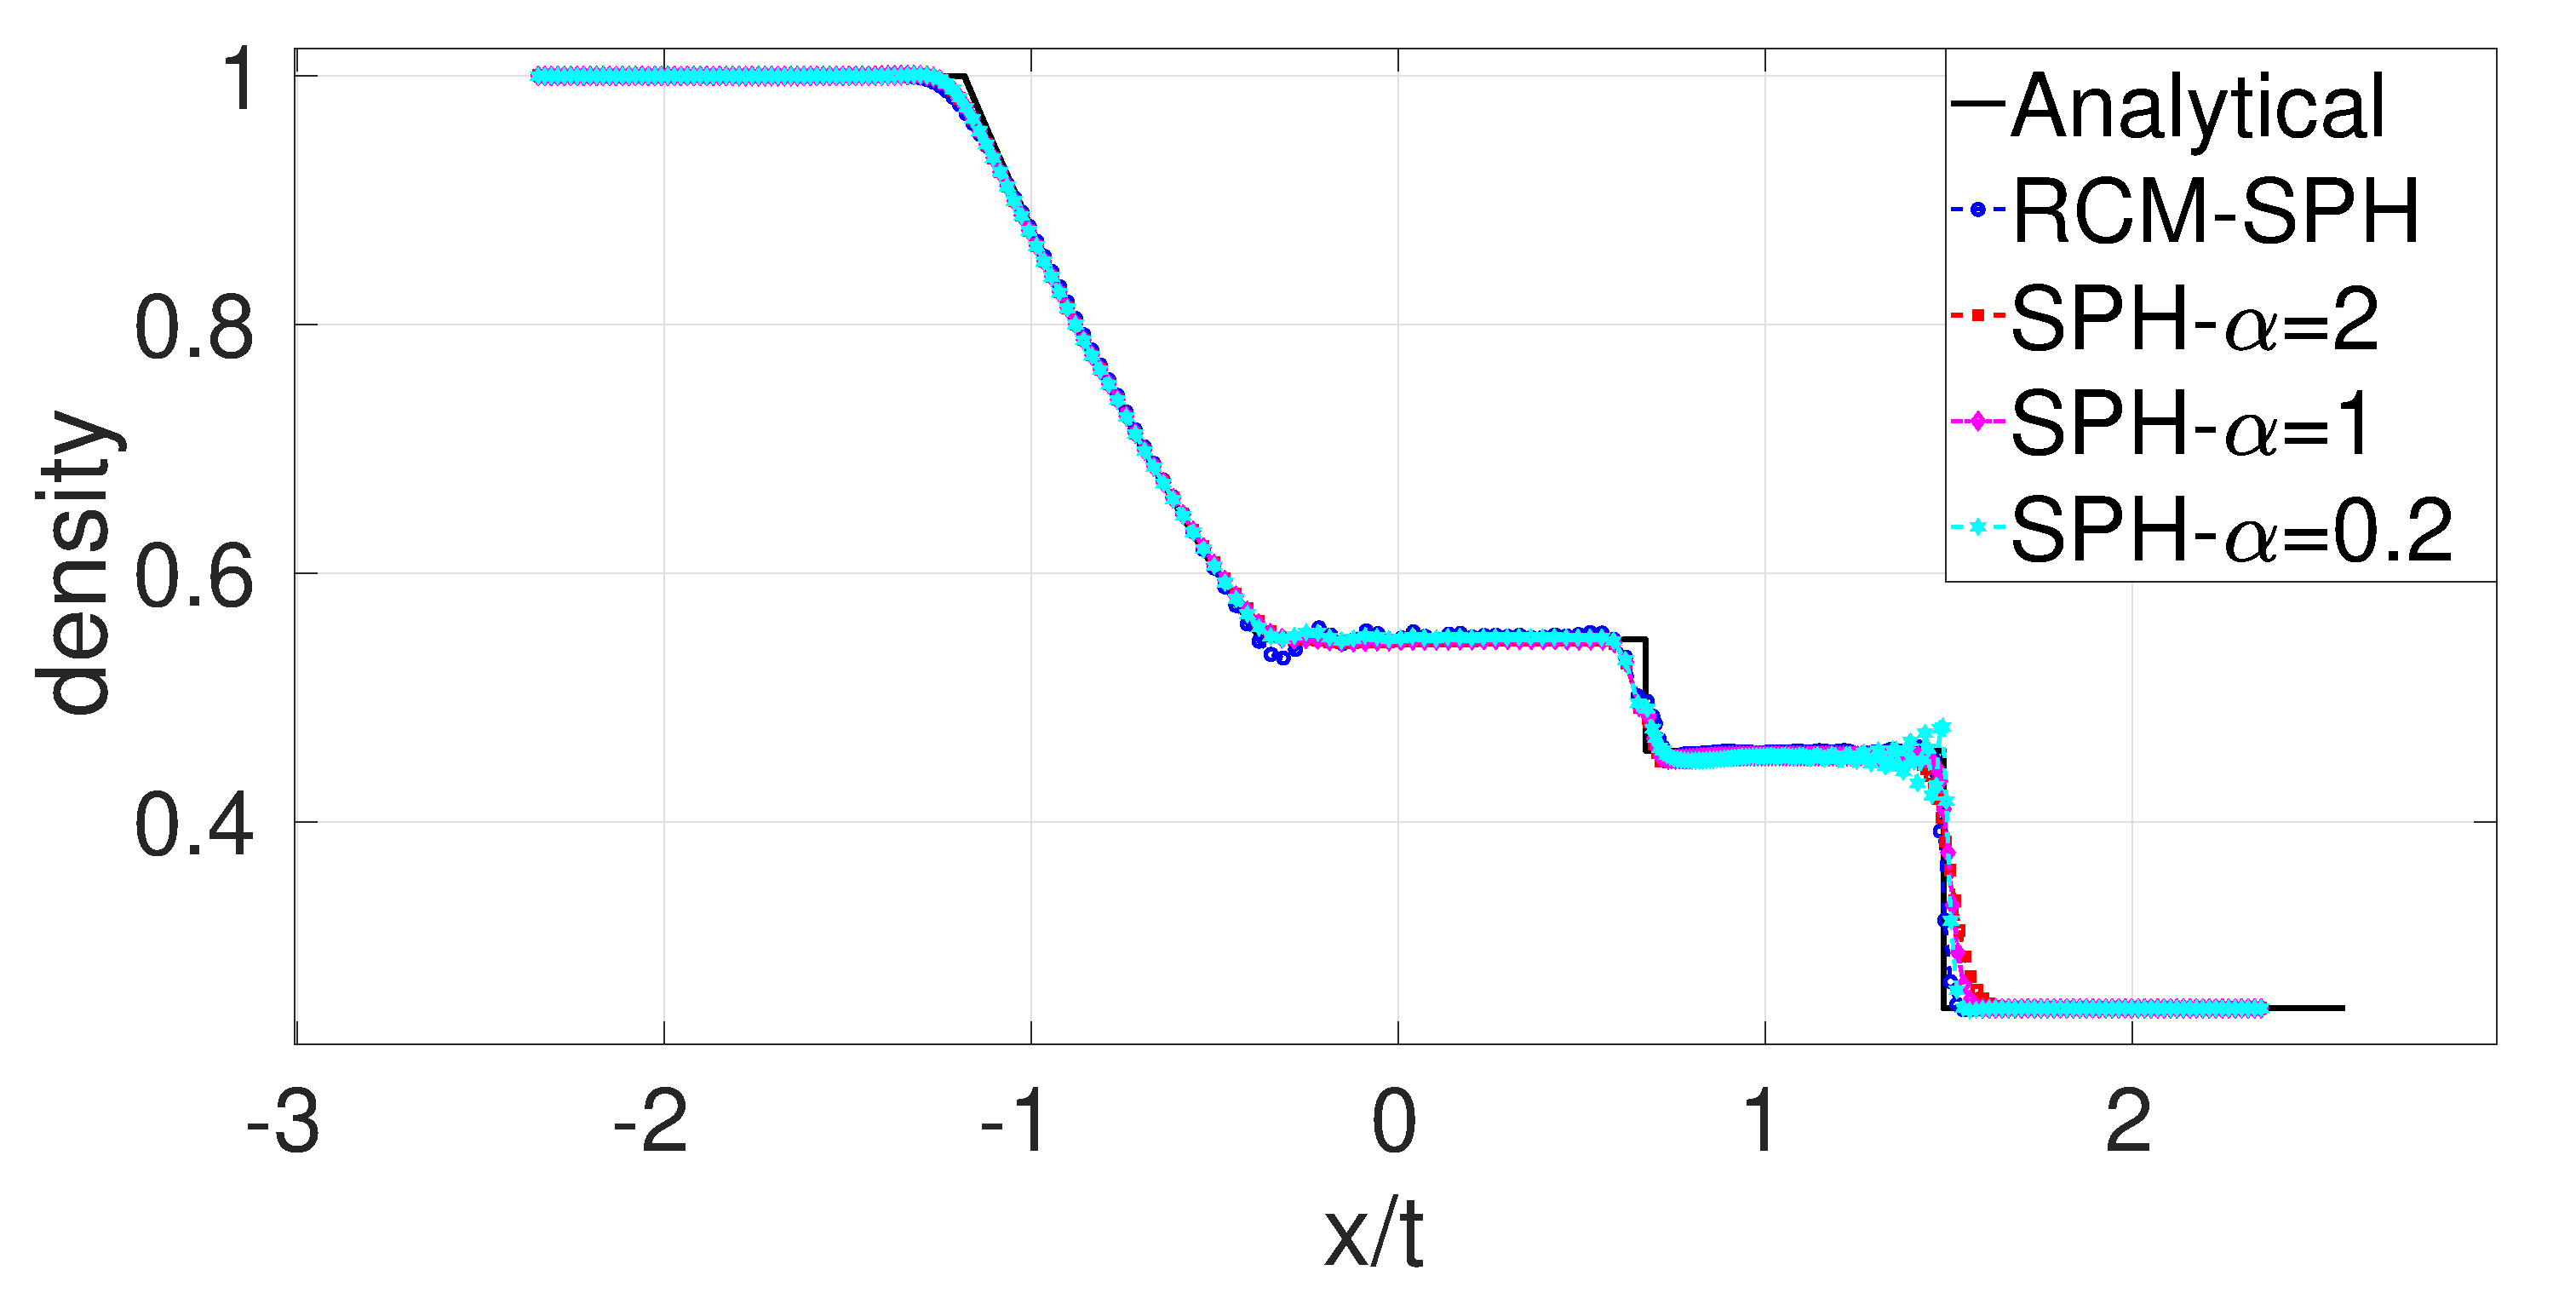
\includegraphics[width=0.90 \textwidth,height=0.7\textwidth]{./Chapter-4/Figures/Sod/RCM-Sod-SPH-alf-rho}
    \end{minipage}%
    \begin{minipage}{.3\textwidth}
        \centering
        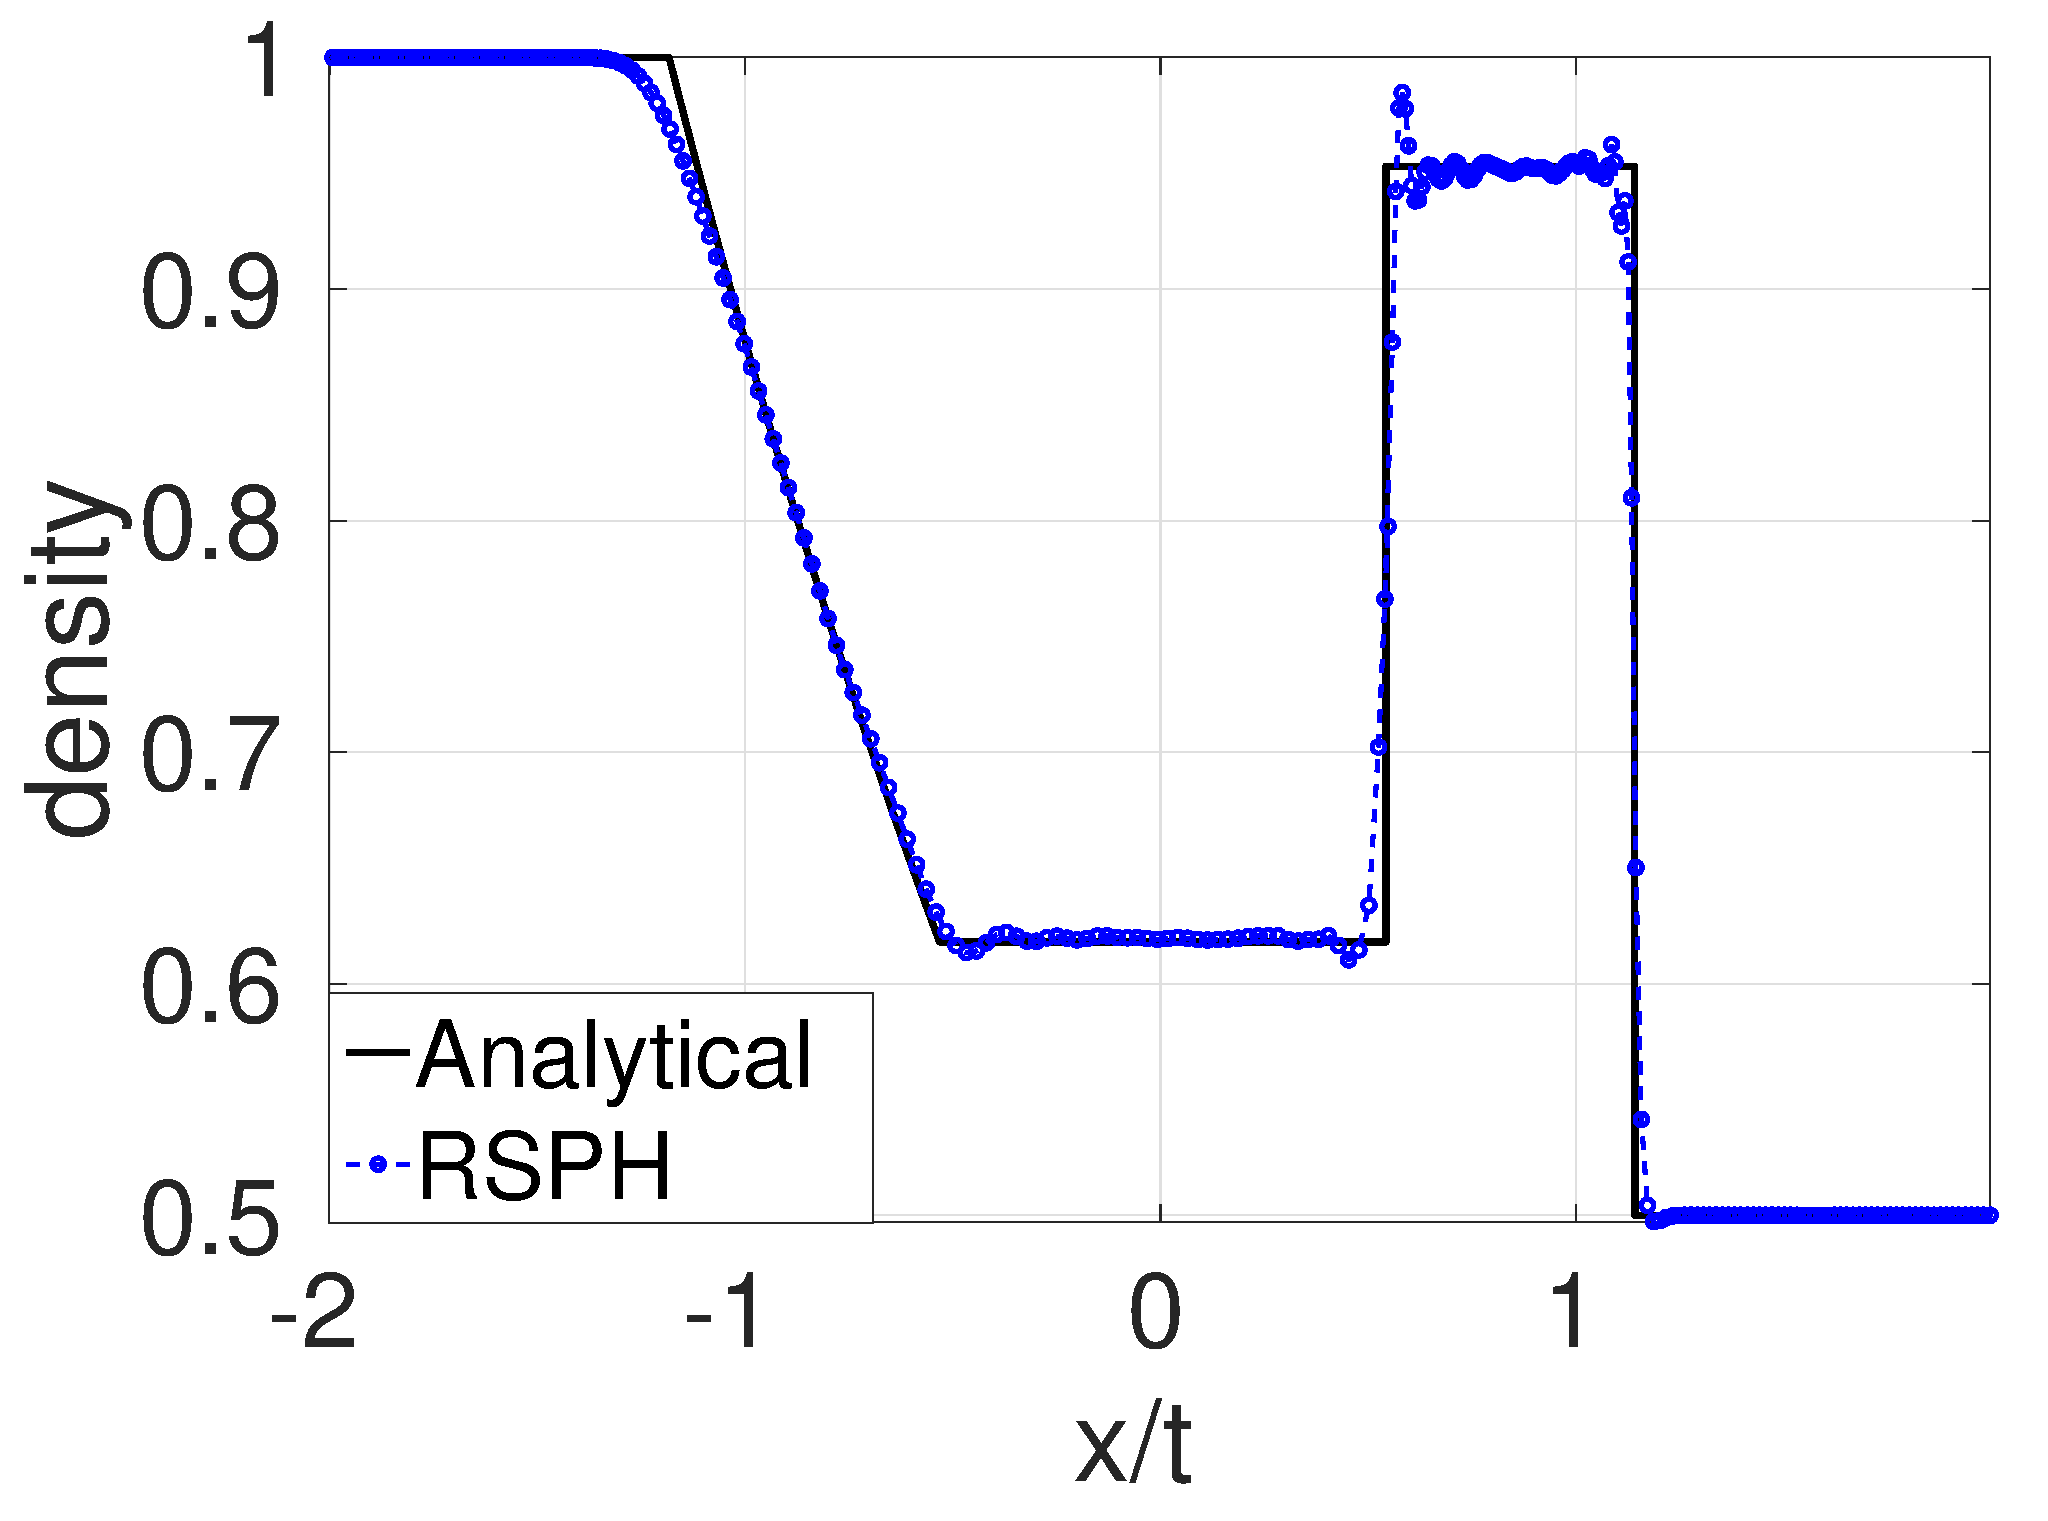
\includegraphics[width=0.90 \textwidth]{./Chapter-4/Figures/GSPH-Sod/GRod-RCM-rho}
    \end{minipage}%  
    \begin{minipage}{.3\textwidth}
        \centering
        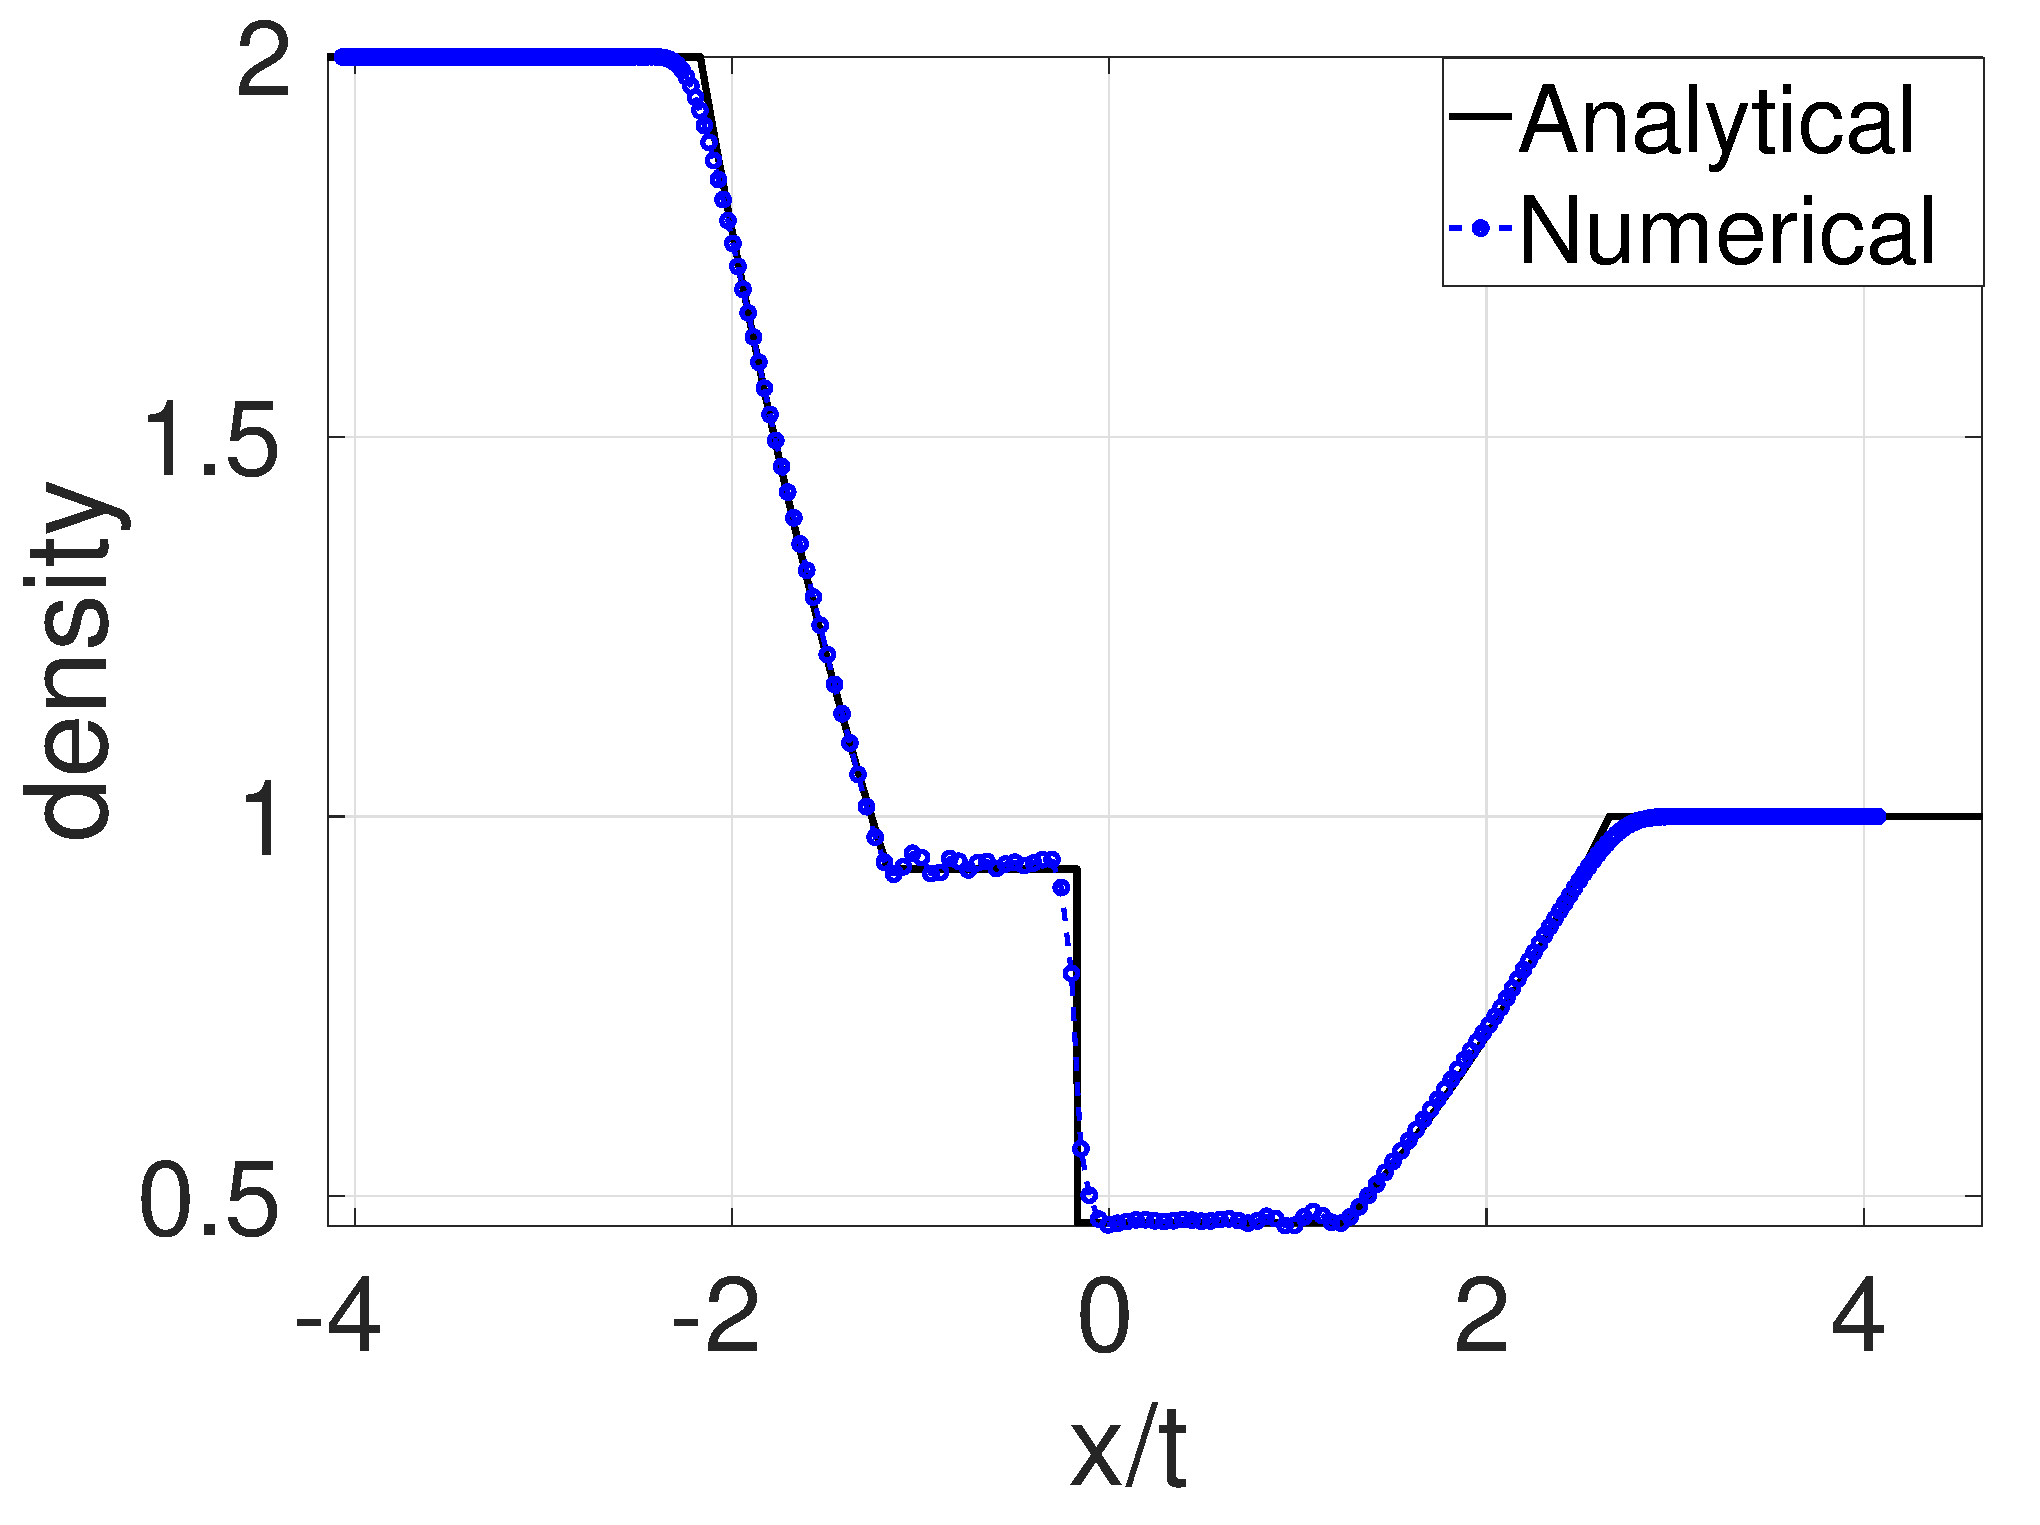
\includegraphics[width=0.90 \textwidth]{./Chapter-4/Figures/double_exp/Dexp-RCM-rho}
    \end{minipage}}% 
   \\
   \center{    
     \begin{minipage}{.3\textwidth}
        \centering
        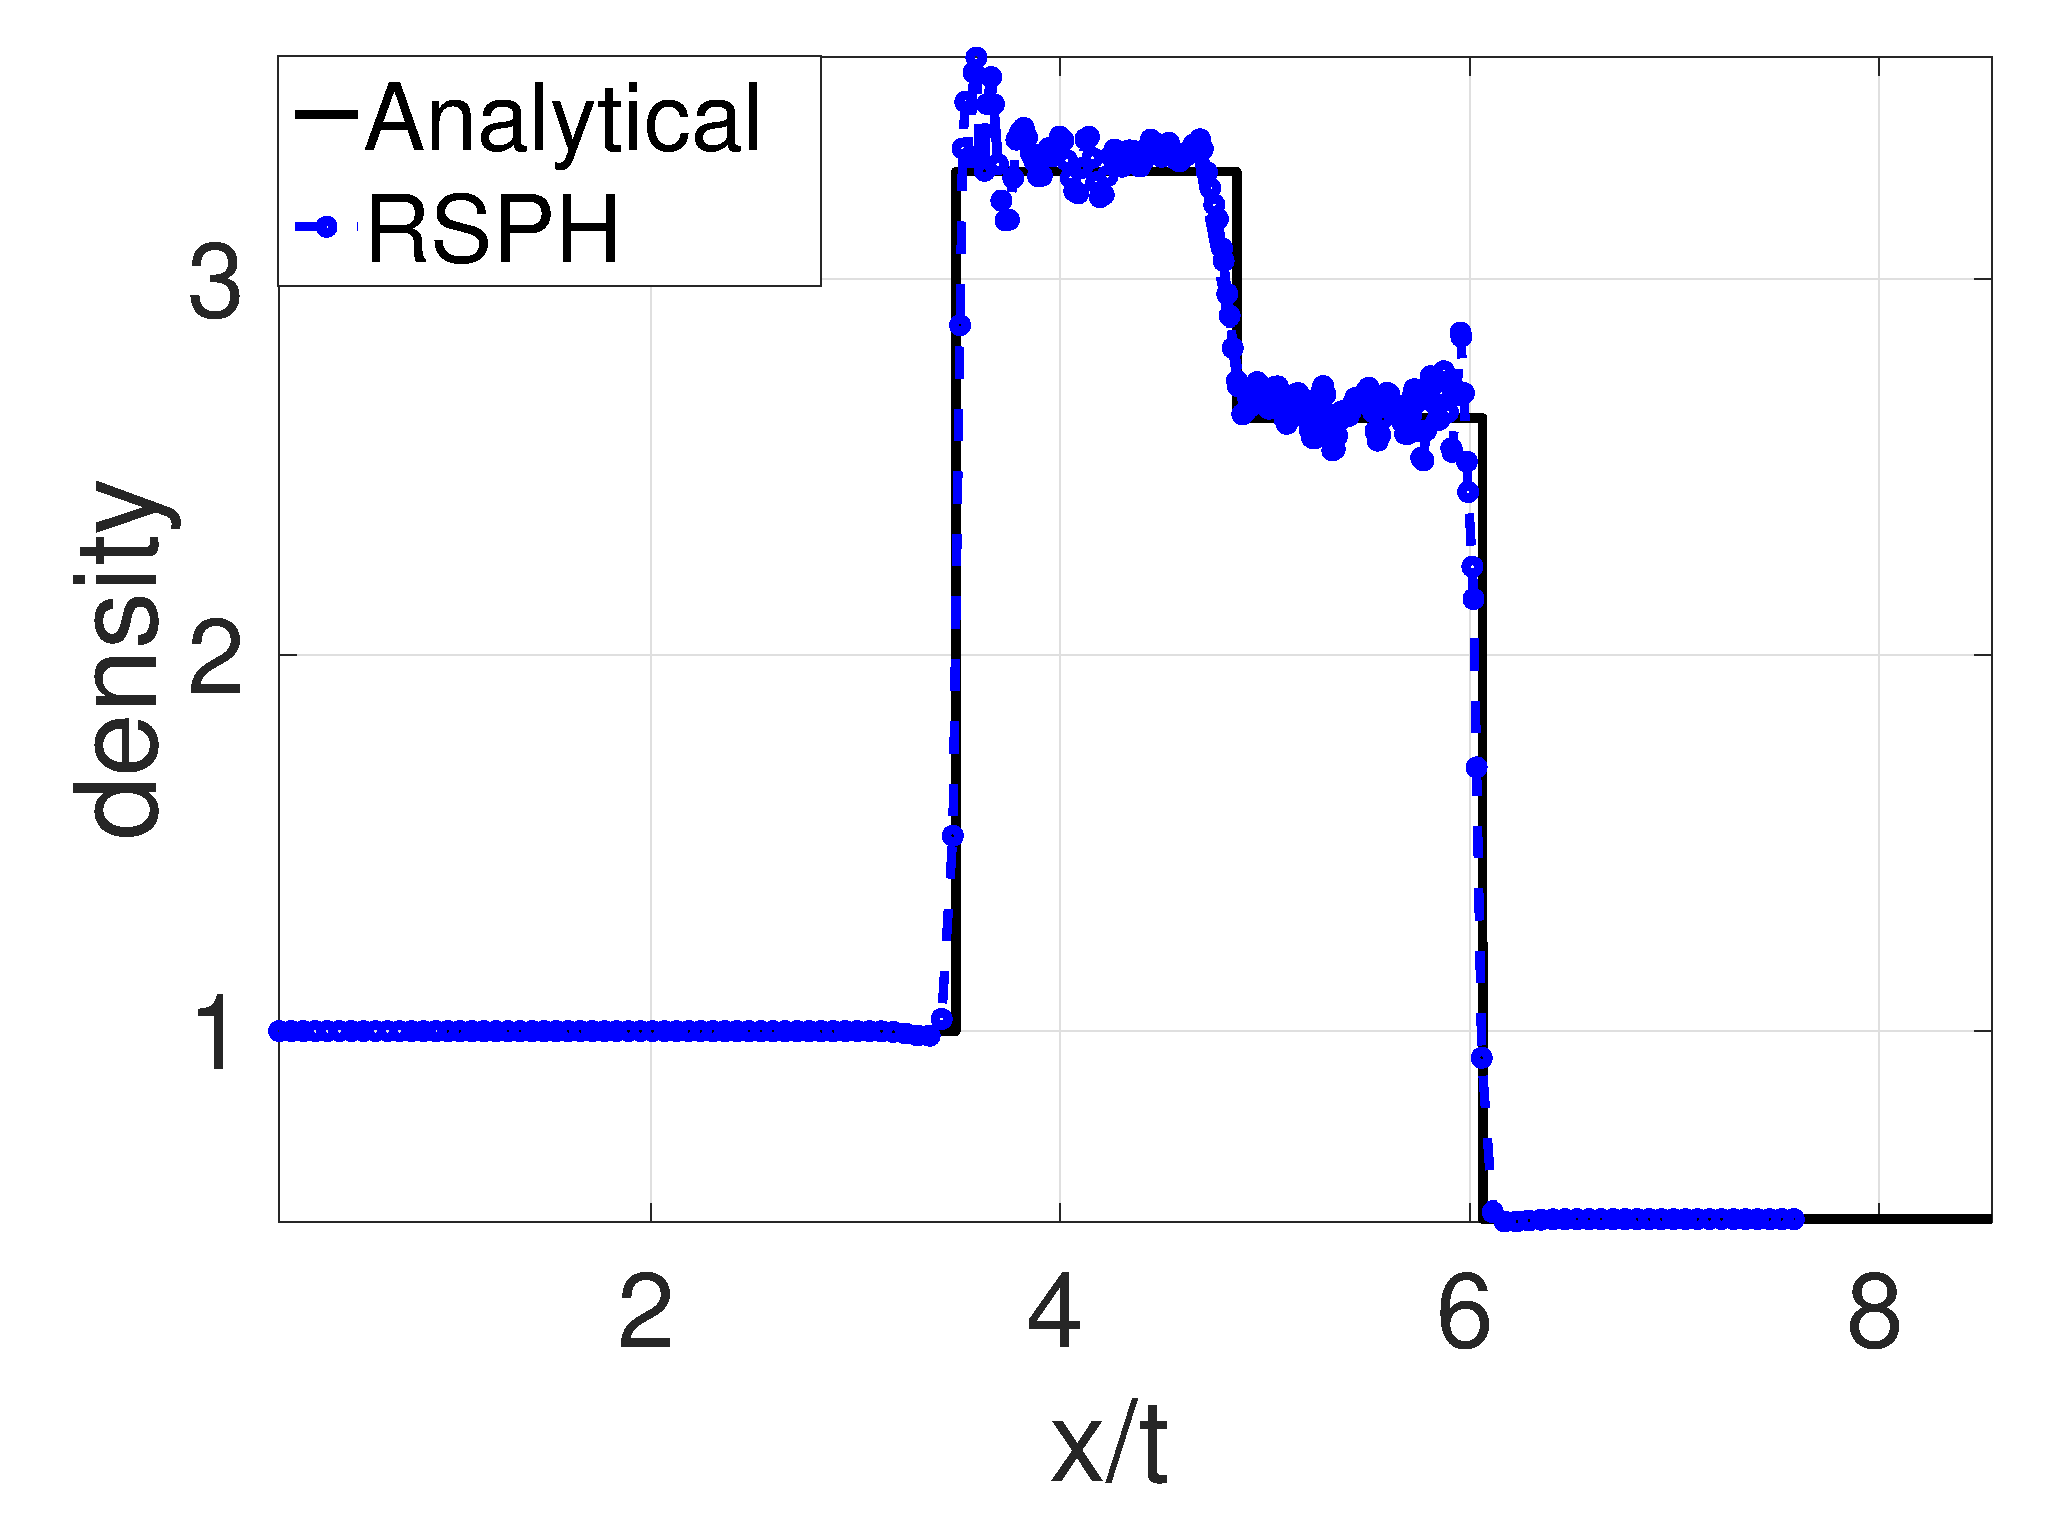
\includegraphics[width=0.90 \textwidth]{./Chapter-4/Figures/double_shock/Dshock-RCM-rho-Rp6}
    \end{minipage}%
    \begin{minipage}{.3\textwidth}
        \centering
        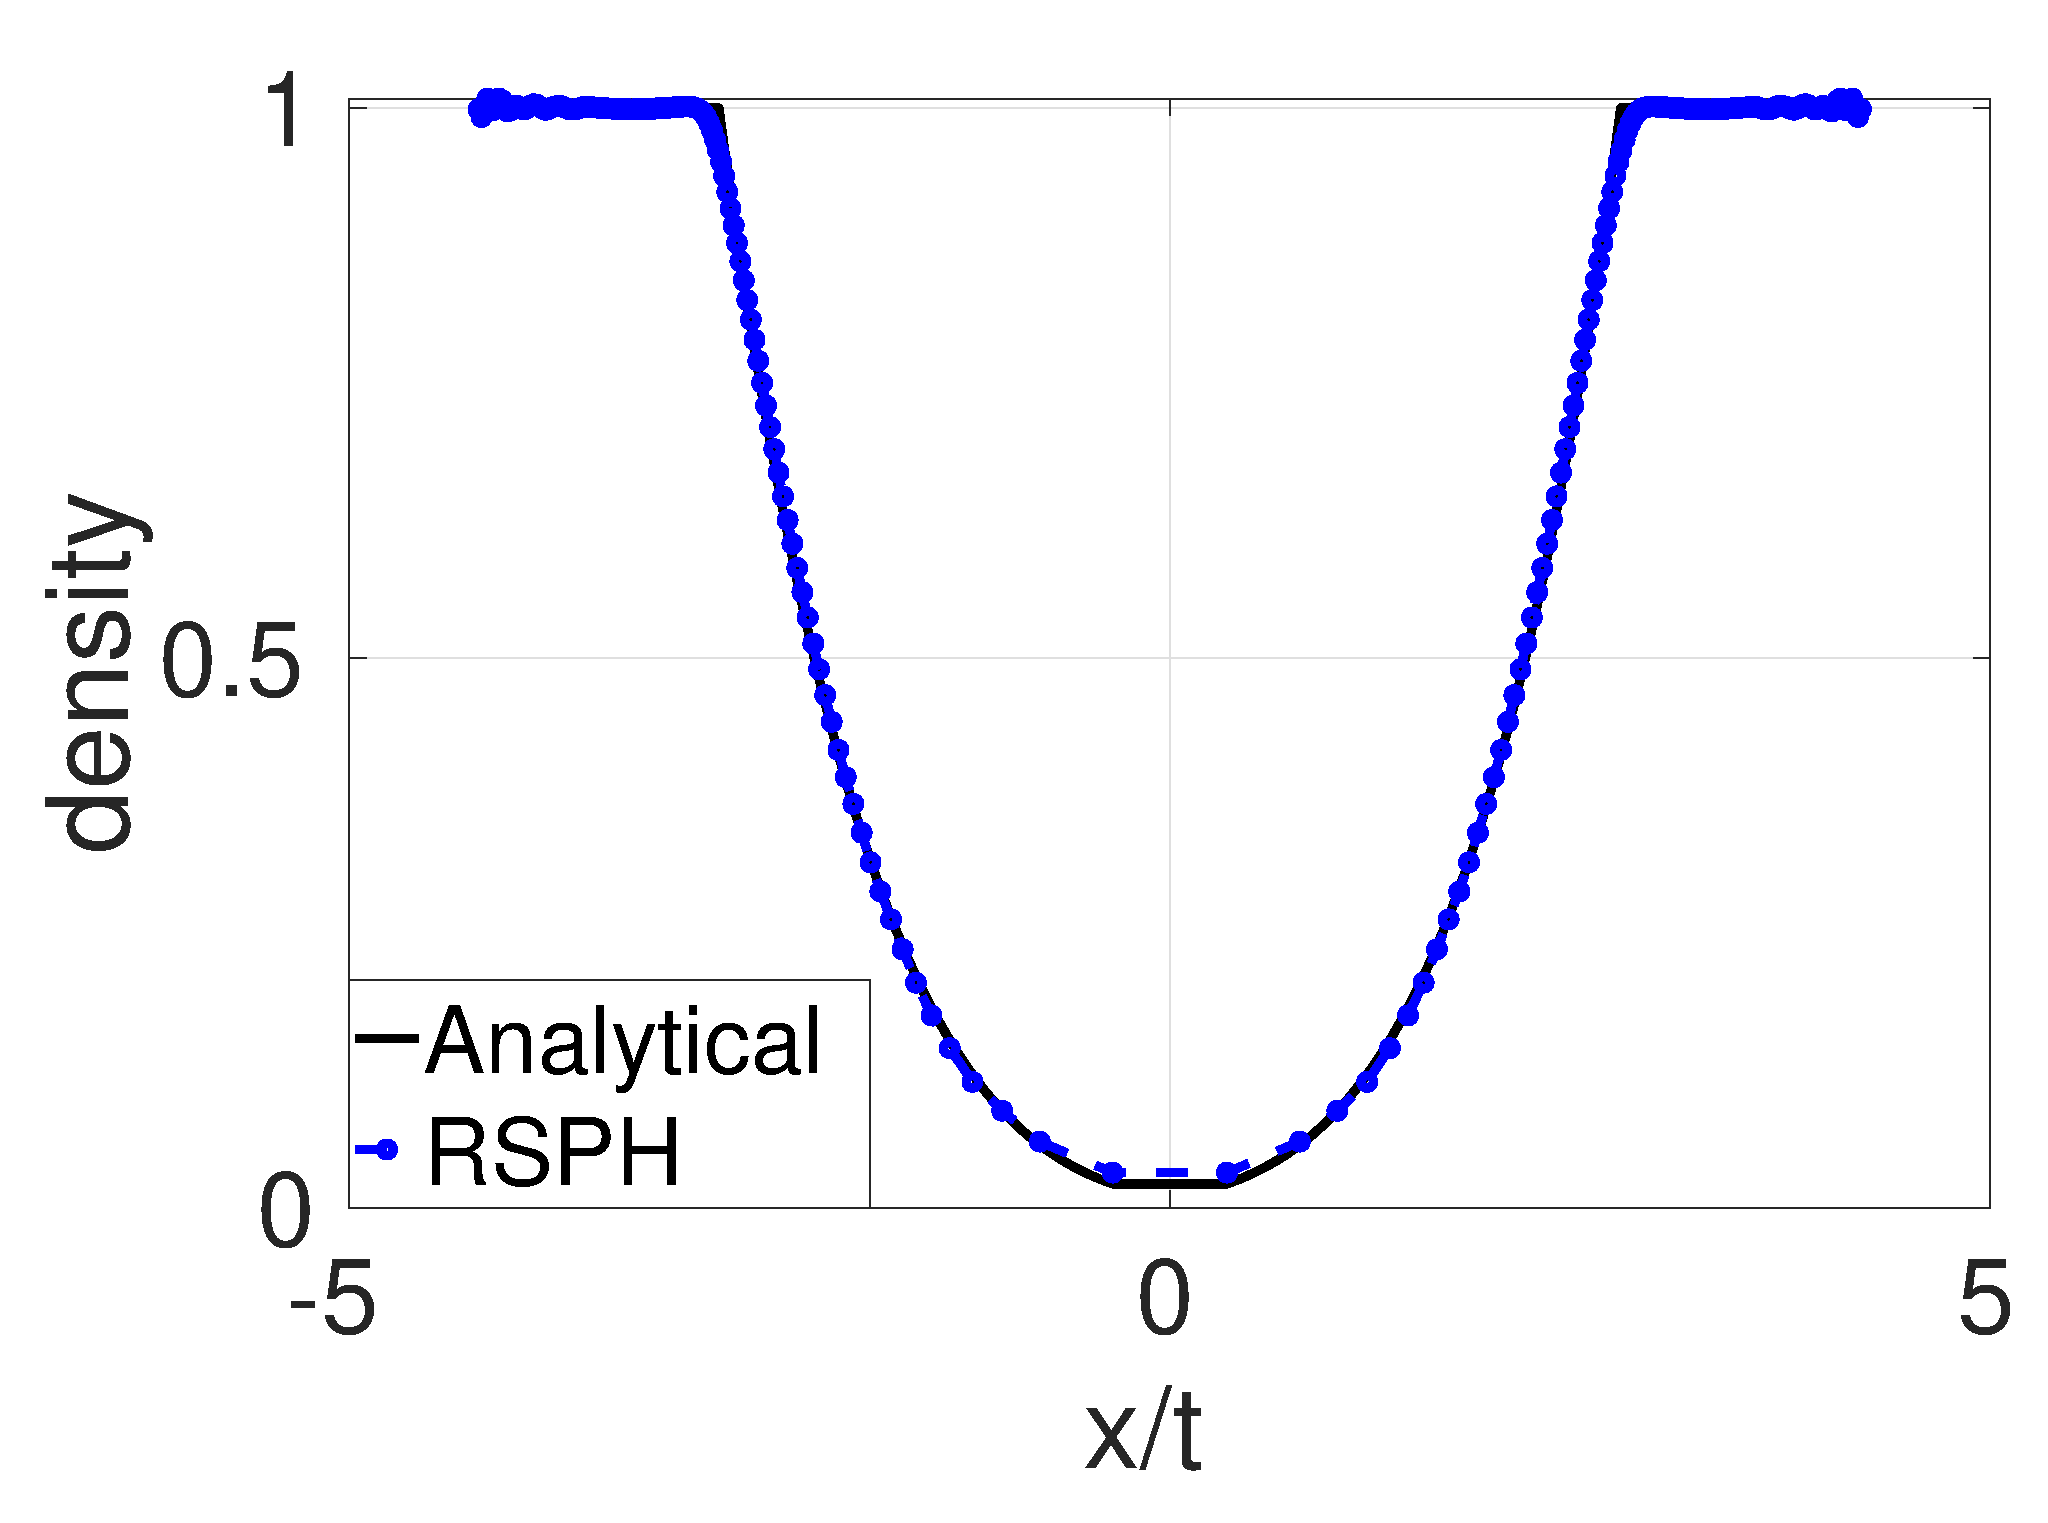
\includegraphics[width=0.90 \textwidth]{./Chapter-4/Figures/Sjogreen/Sjogreen-RCM-rho-Adpt1}
    \end{minipage}% 
    \begin{minipage}{.3\textwidth}
        \centering
        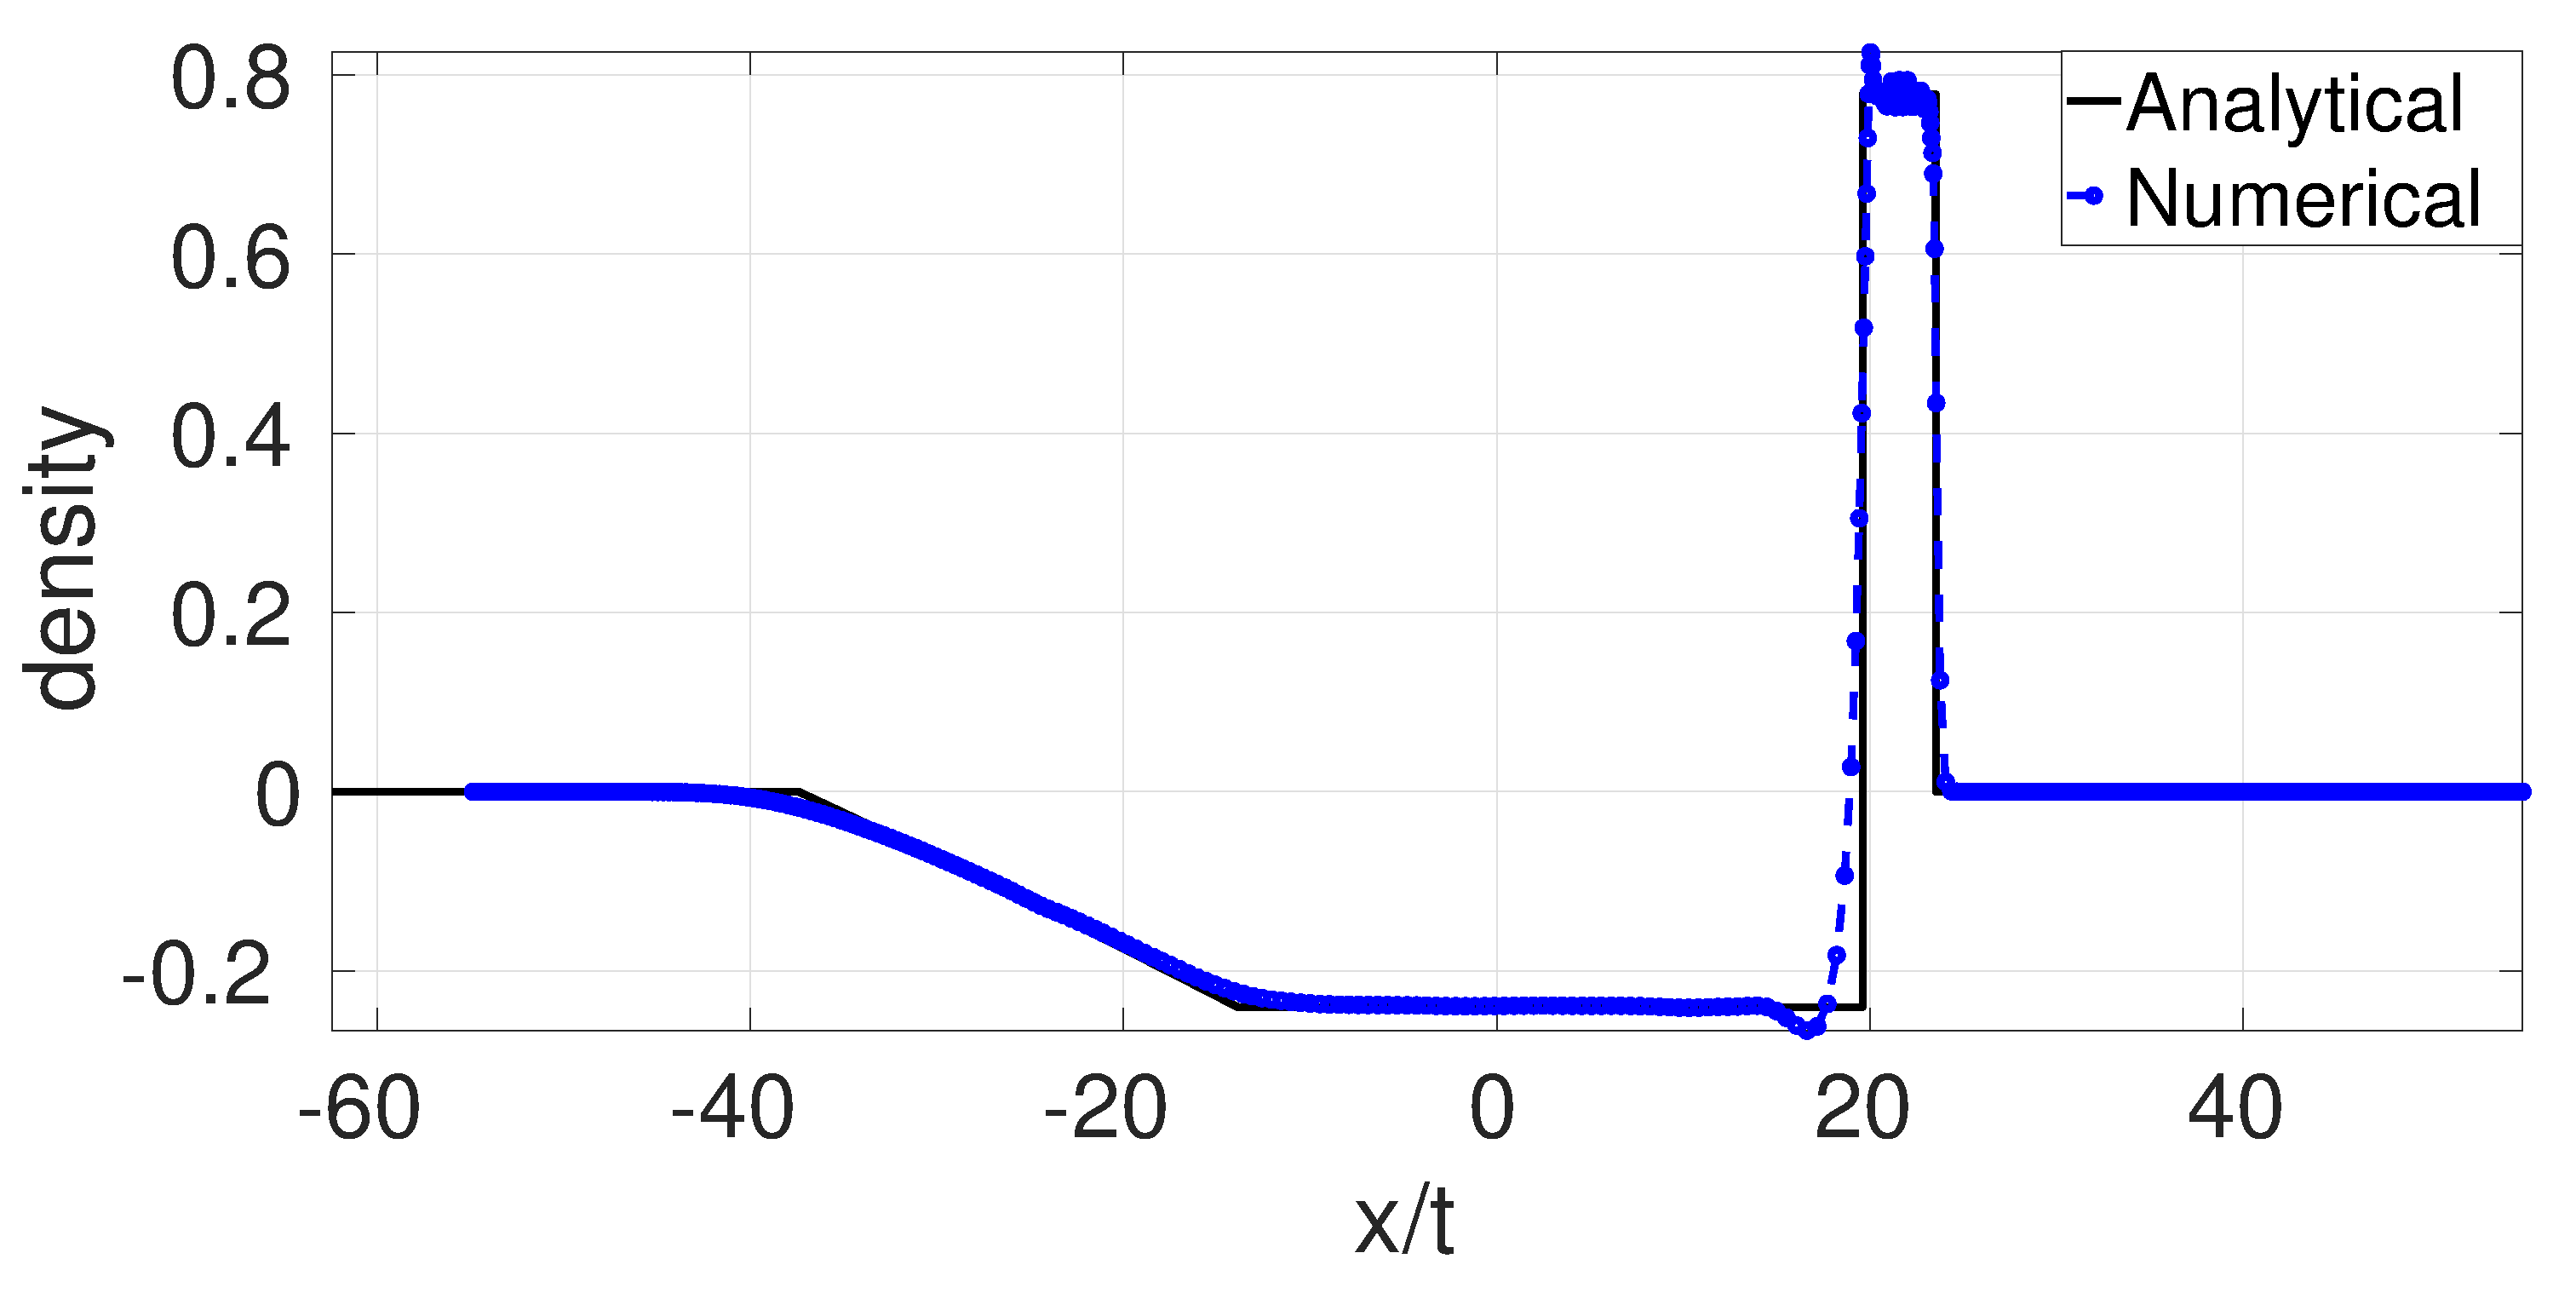
\includegraphics[width=0.90 \textwidth]{./Chapter-4/Figures/strong-blast/StrBlst-RCM-rho-Rp3}
    \end{minipage}}
    \\
\begin{figure}
    \centering
    \begin{minipage}{.3\textwidth}
        \centering
        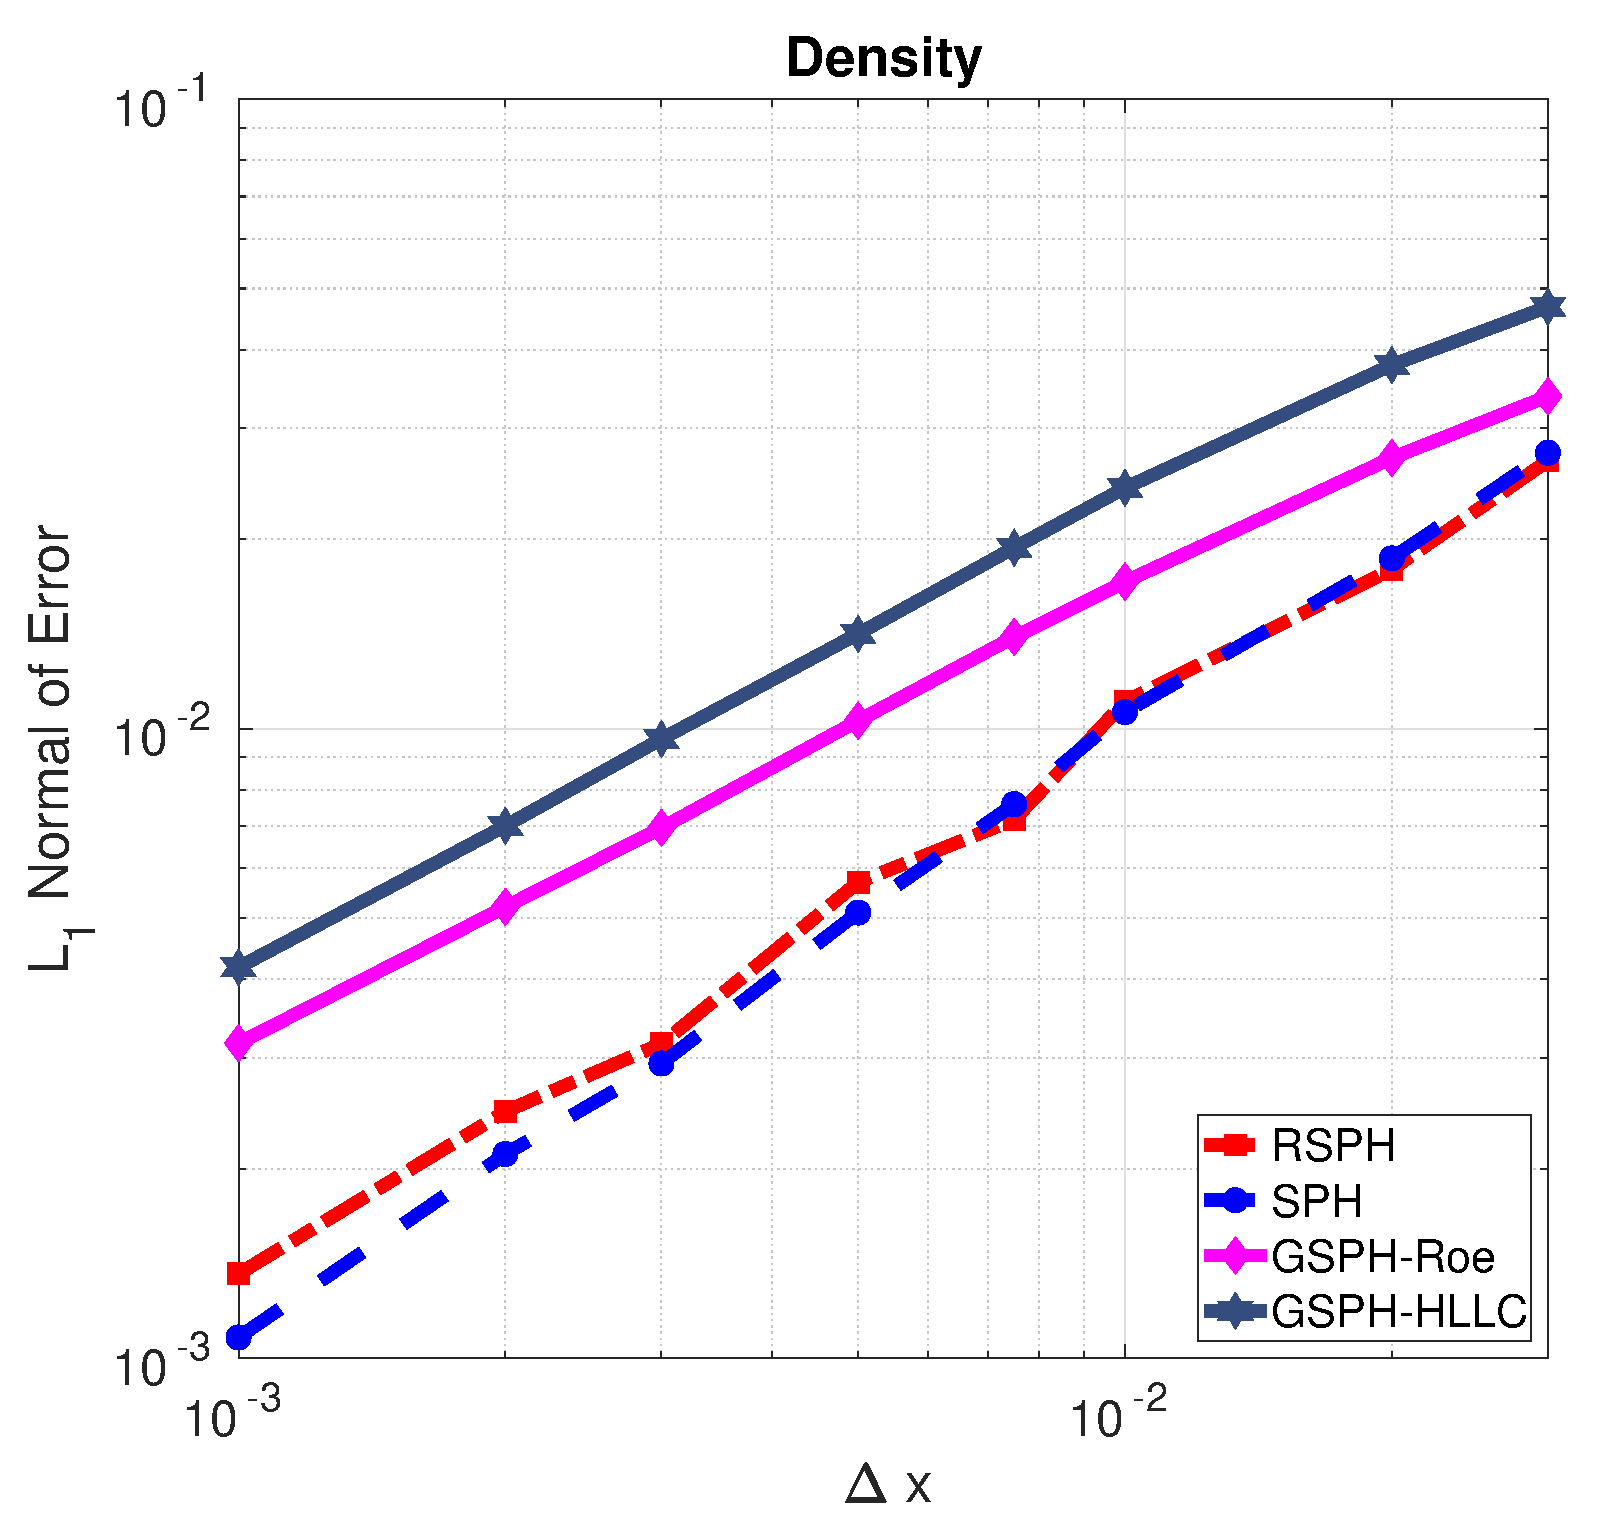
\includegraphics[width=0.95 \textwidth]{./Chapter-4/Figures/Accuracy-des}
    \end{minipage}%
    \begin{minipage}{.3 \textwidth}
        \centering
        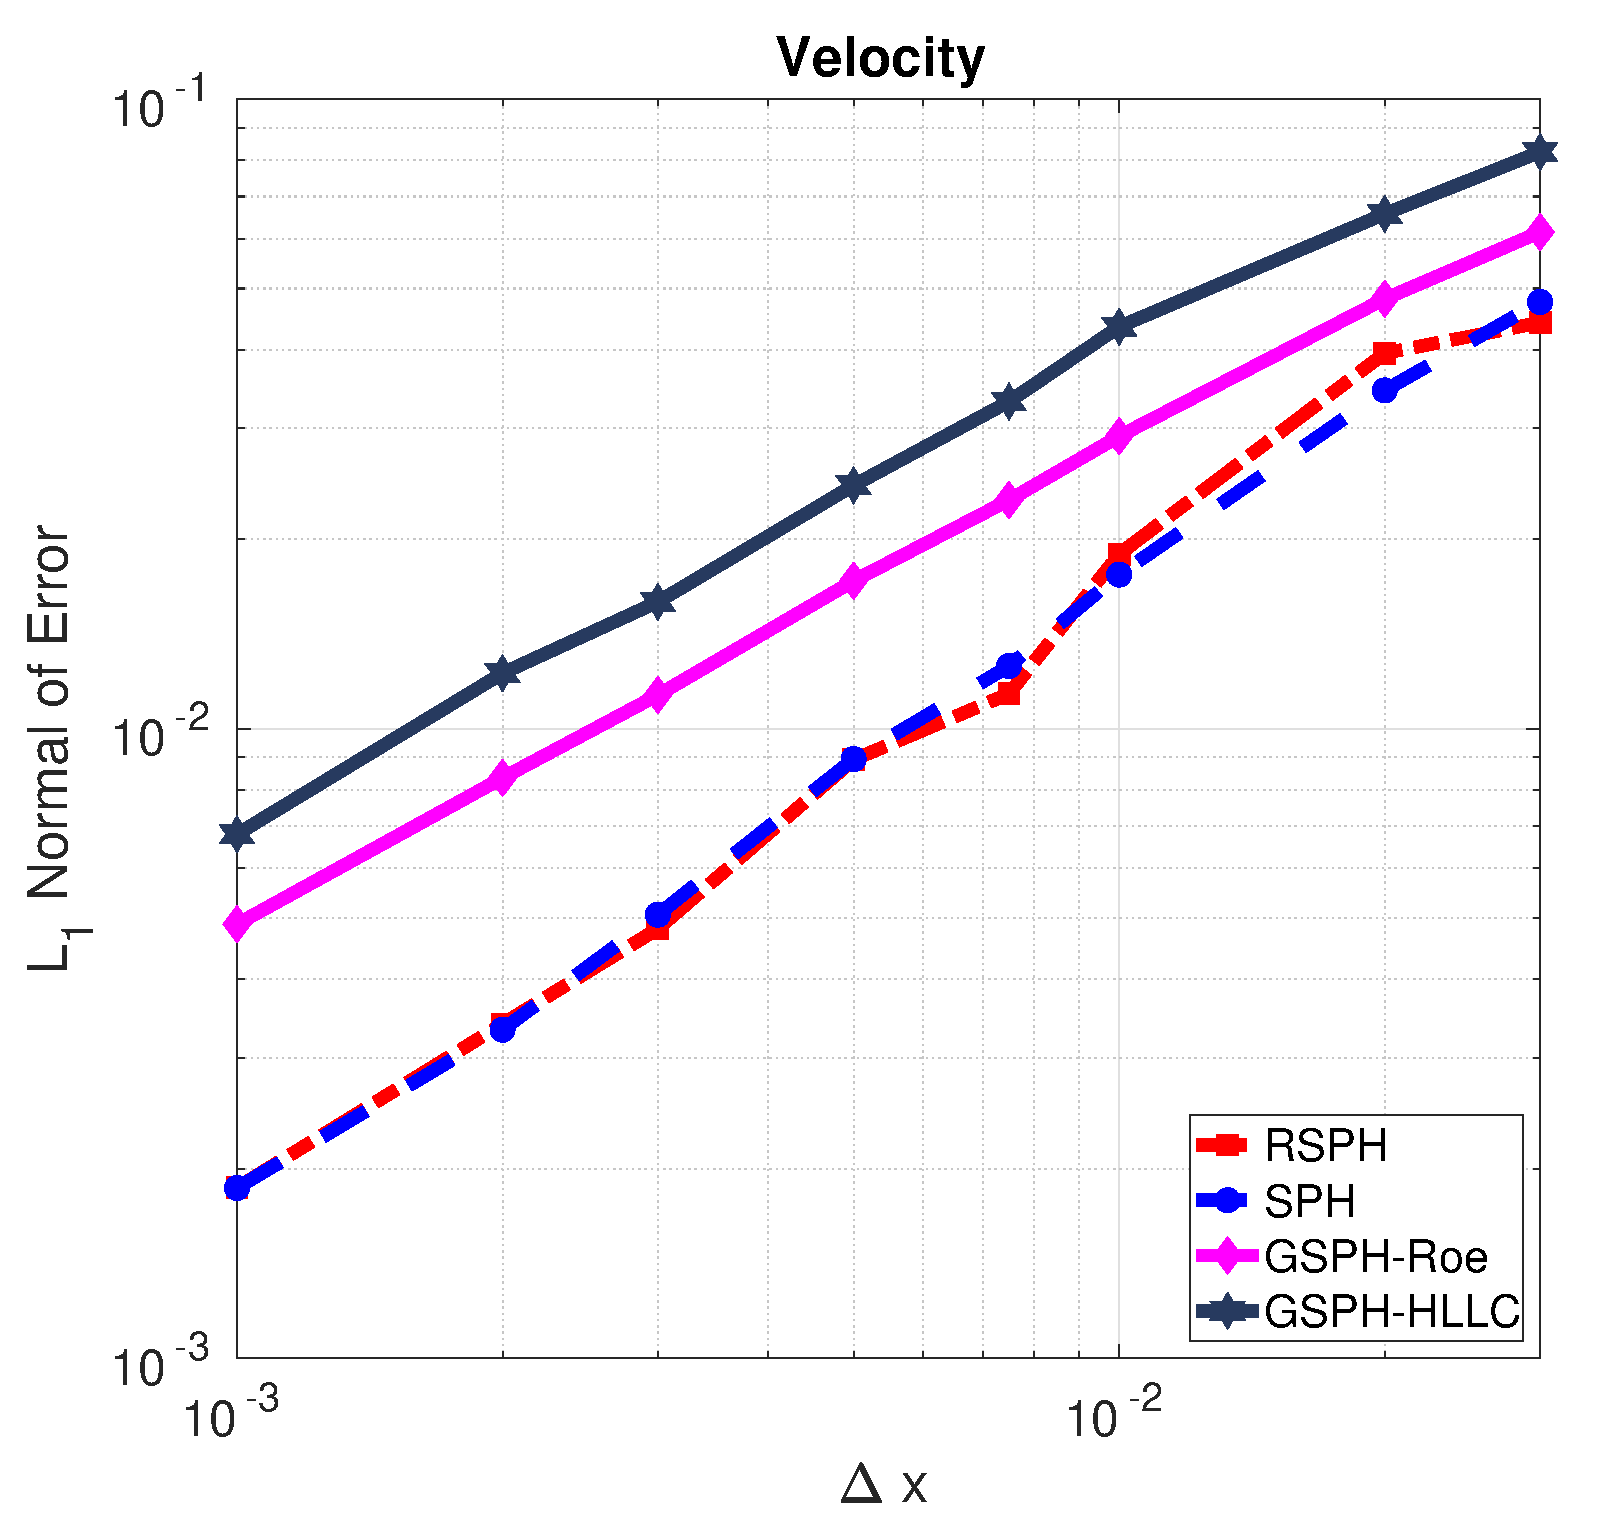
\includegraphics[width=0.95 \textwidth]{./Chapter-4/Figures/Accuracy-vel}
    \end{minipage}%
    \begin{minipage}{.3 \textwidth}
        \centering
        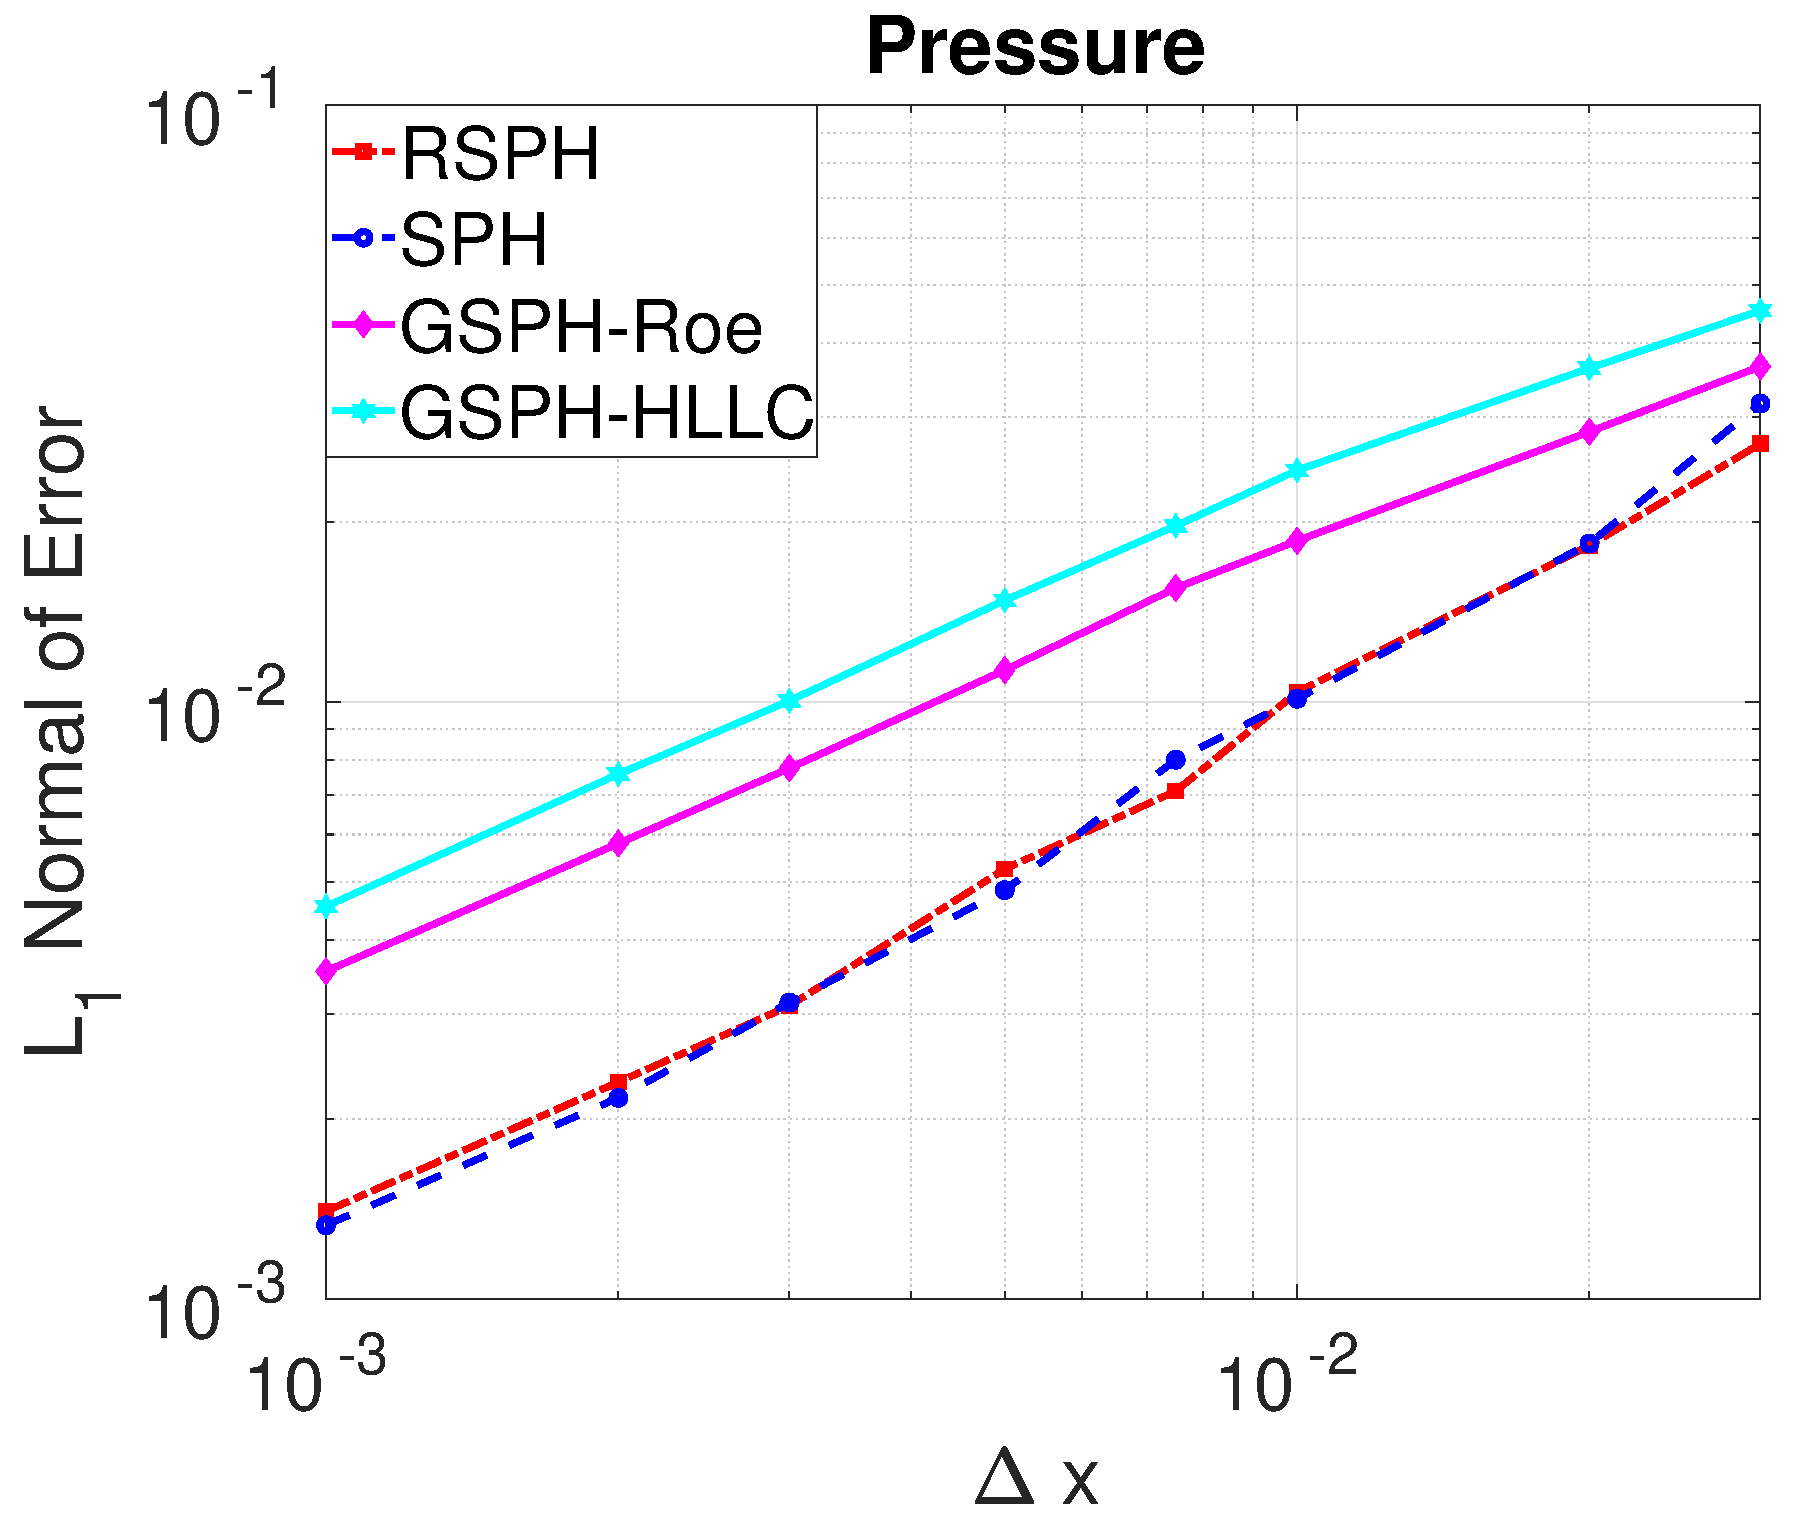
\includegraphics[width=0.95 \textwidth]{./Chapter-4/Figures/Accuracy-pre}
    \end{minipage}%  
\end{figure}     
\end{frame}
%
\begin{frame}{GSPH Vs RSPH}
\begin{figure}[t]
    \centering
    \begin{minipage}{.33 \textwidth}
        \centering
        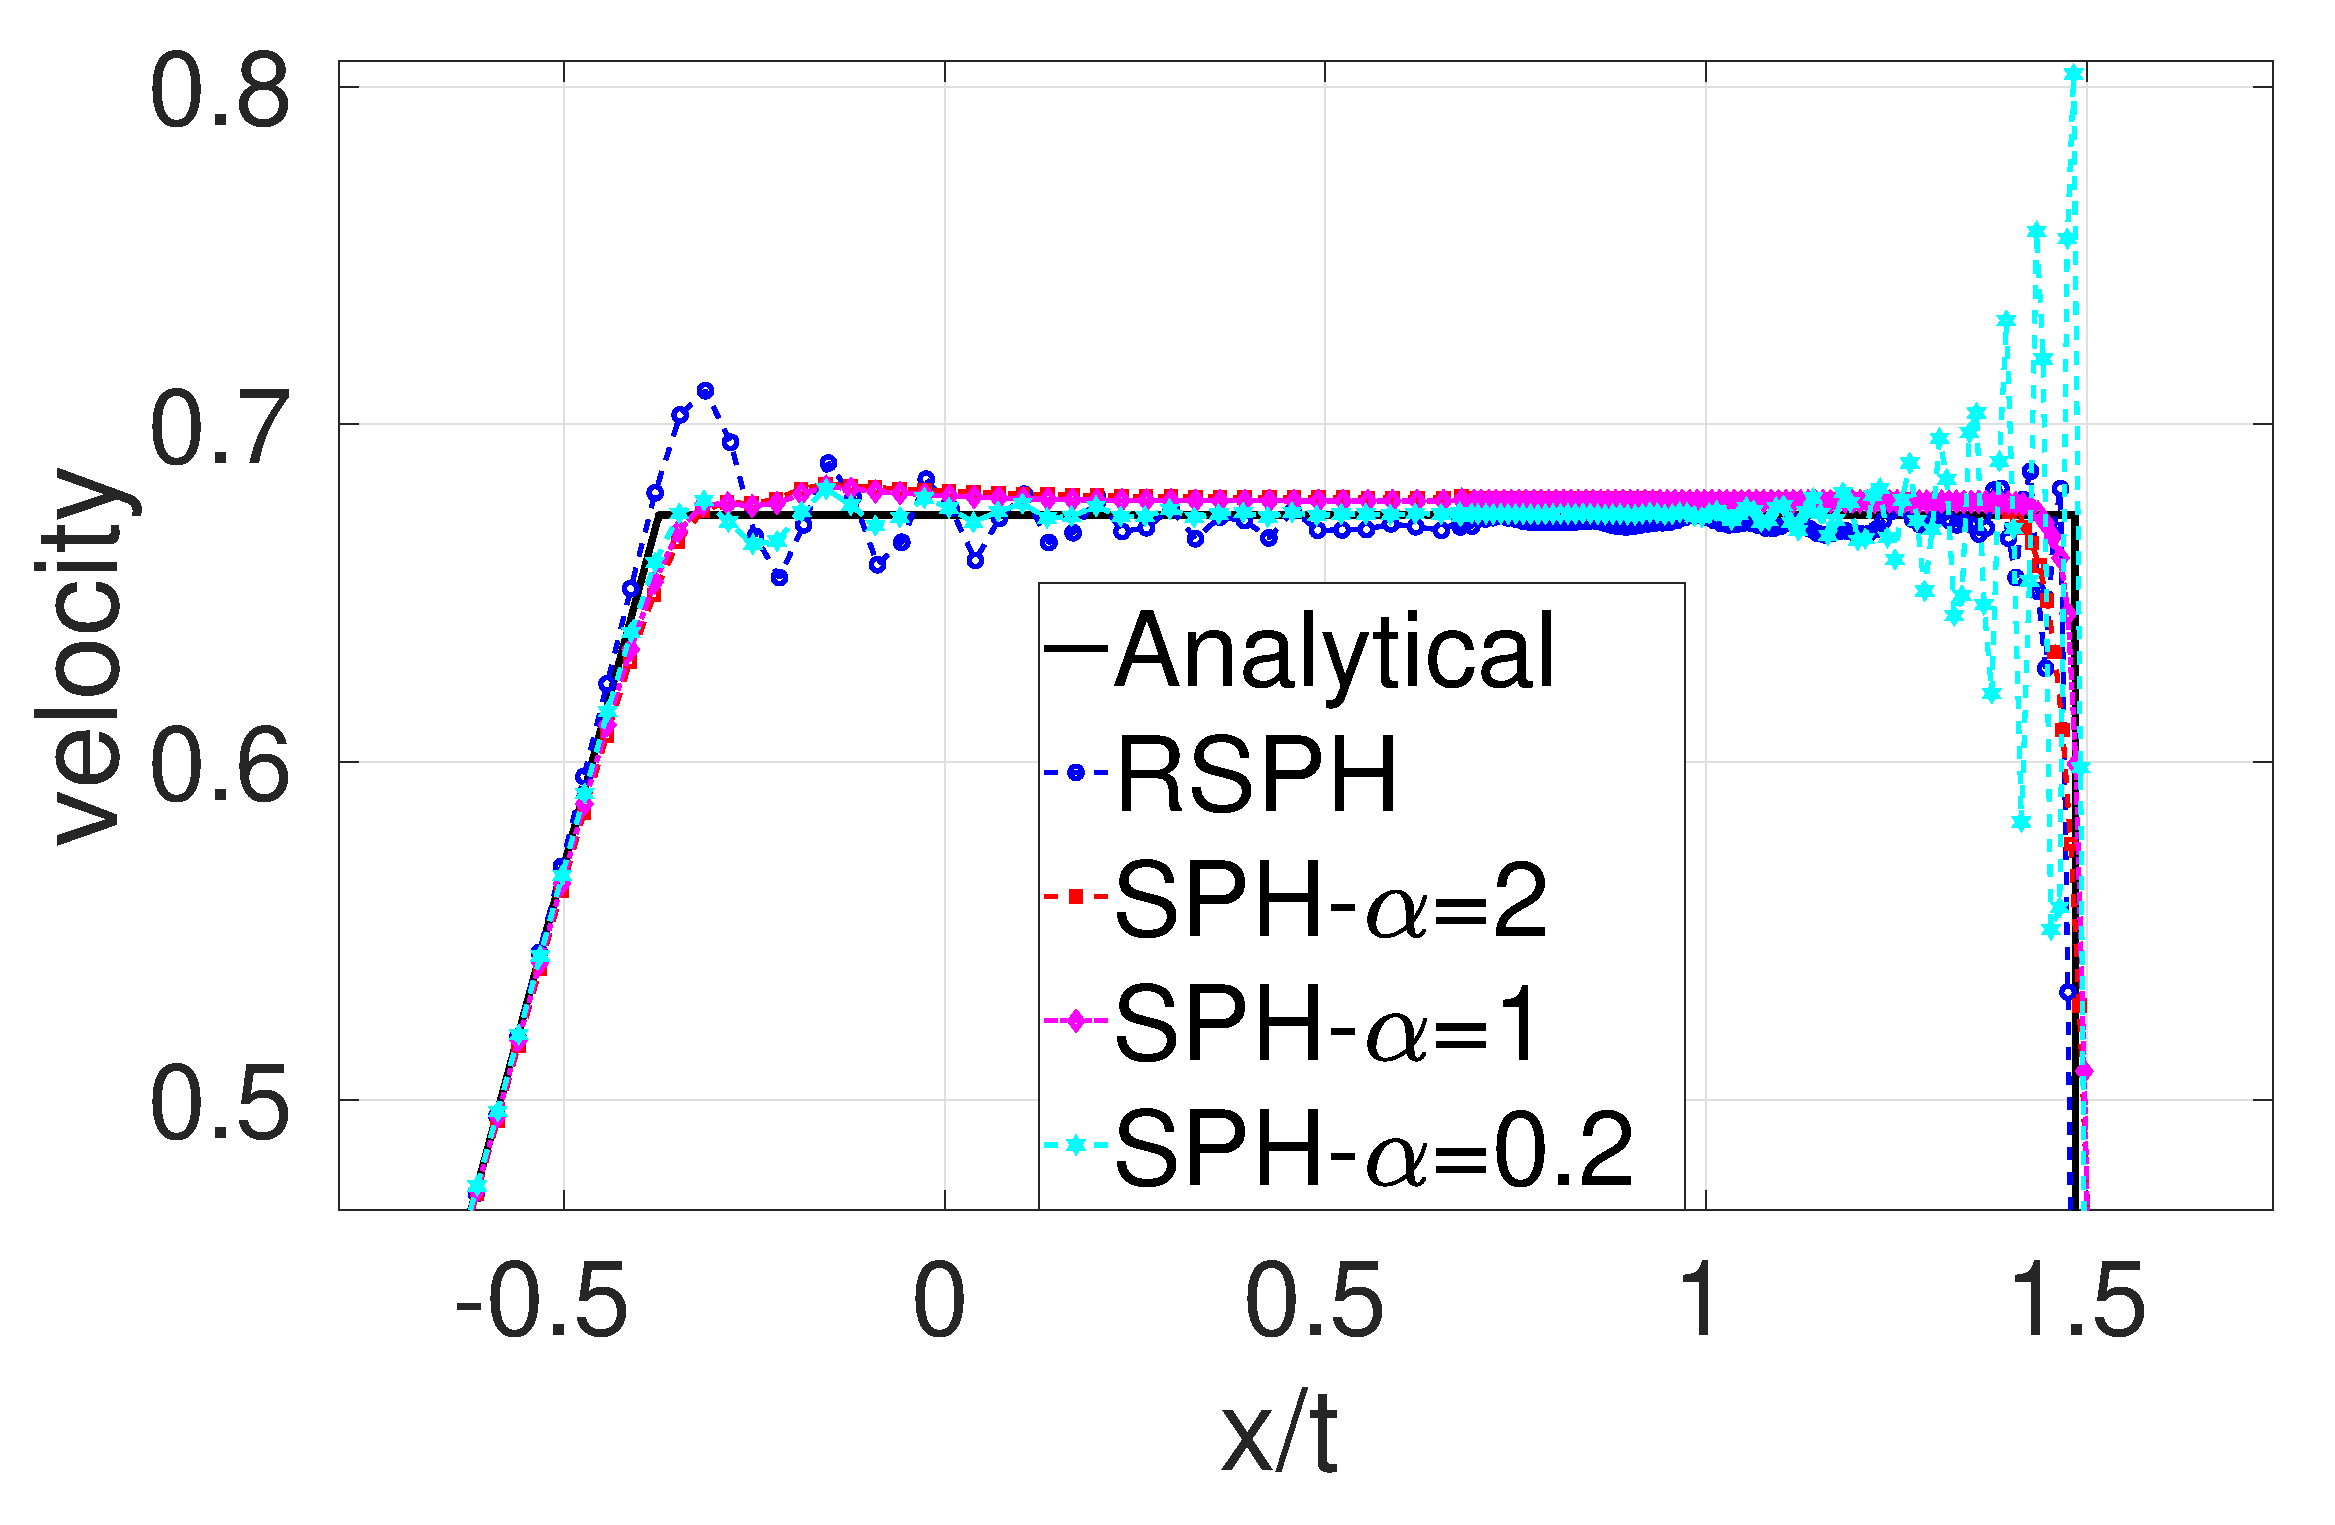
\includegraphics[width=0.99 \textwidth]{./Chapter-4/Figures/Sod/RCM-Sod-SPH-alf-v-zoom}
    \end{minipage}% 
    \begin{minipage}{.33 \textwidth}
        \centering
        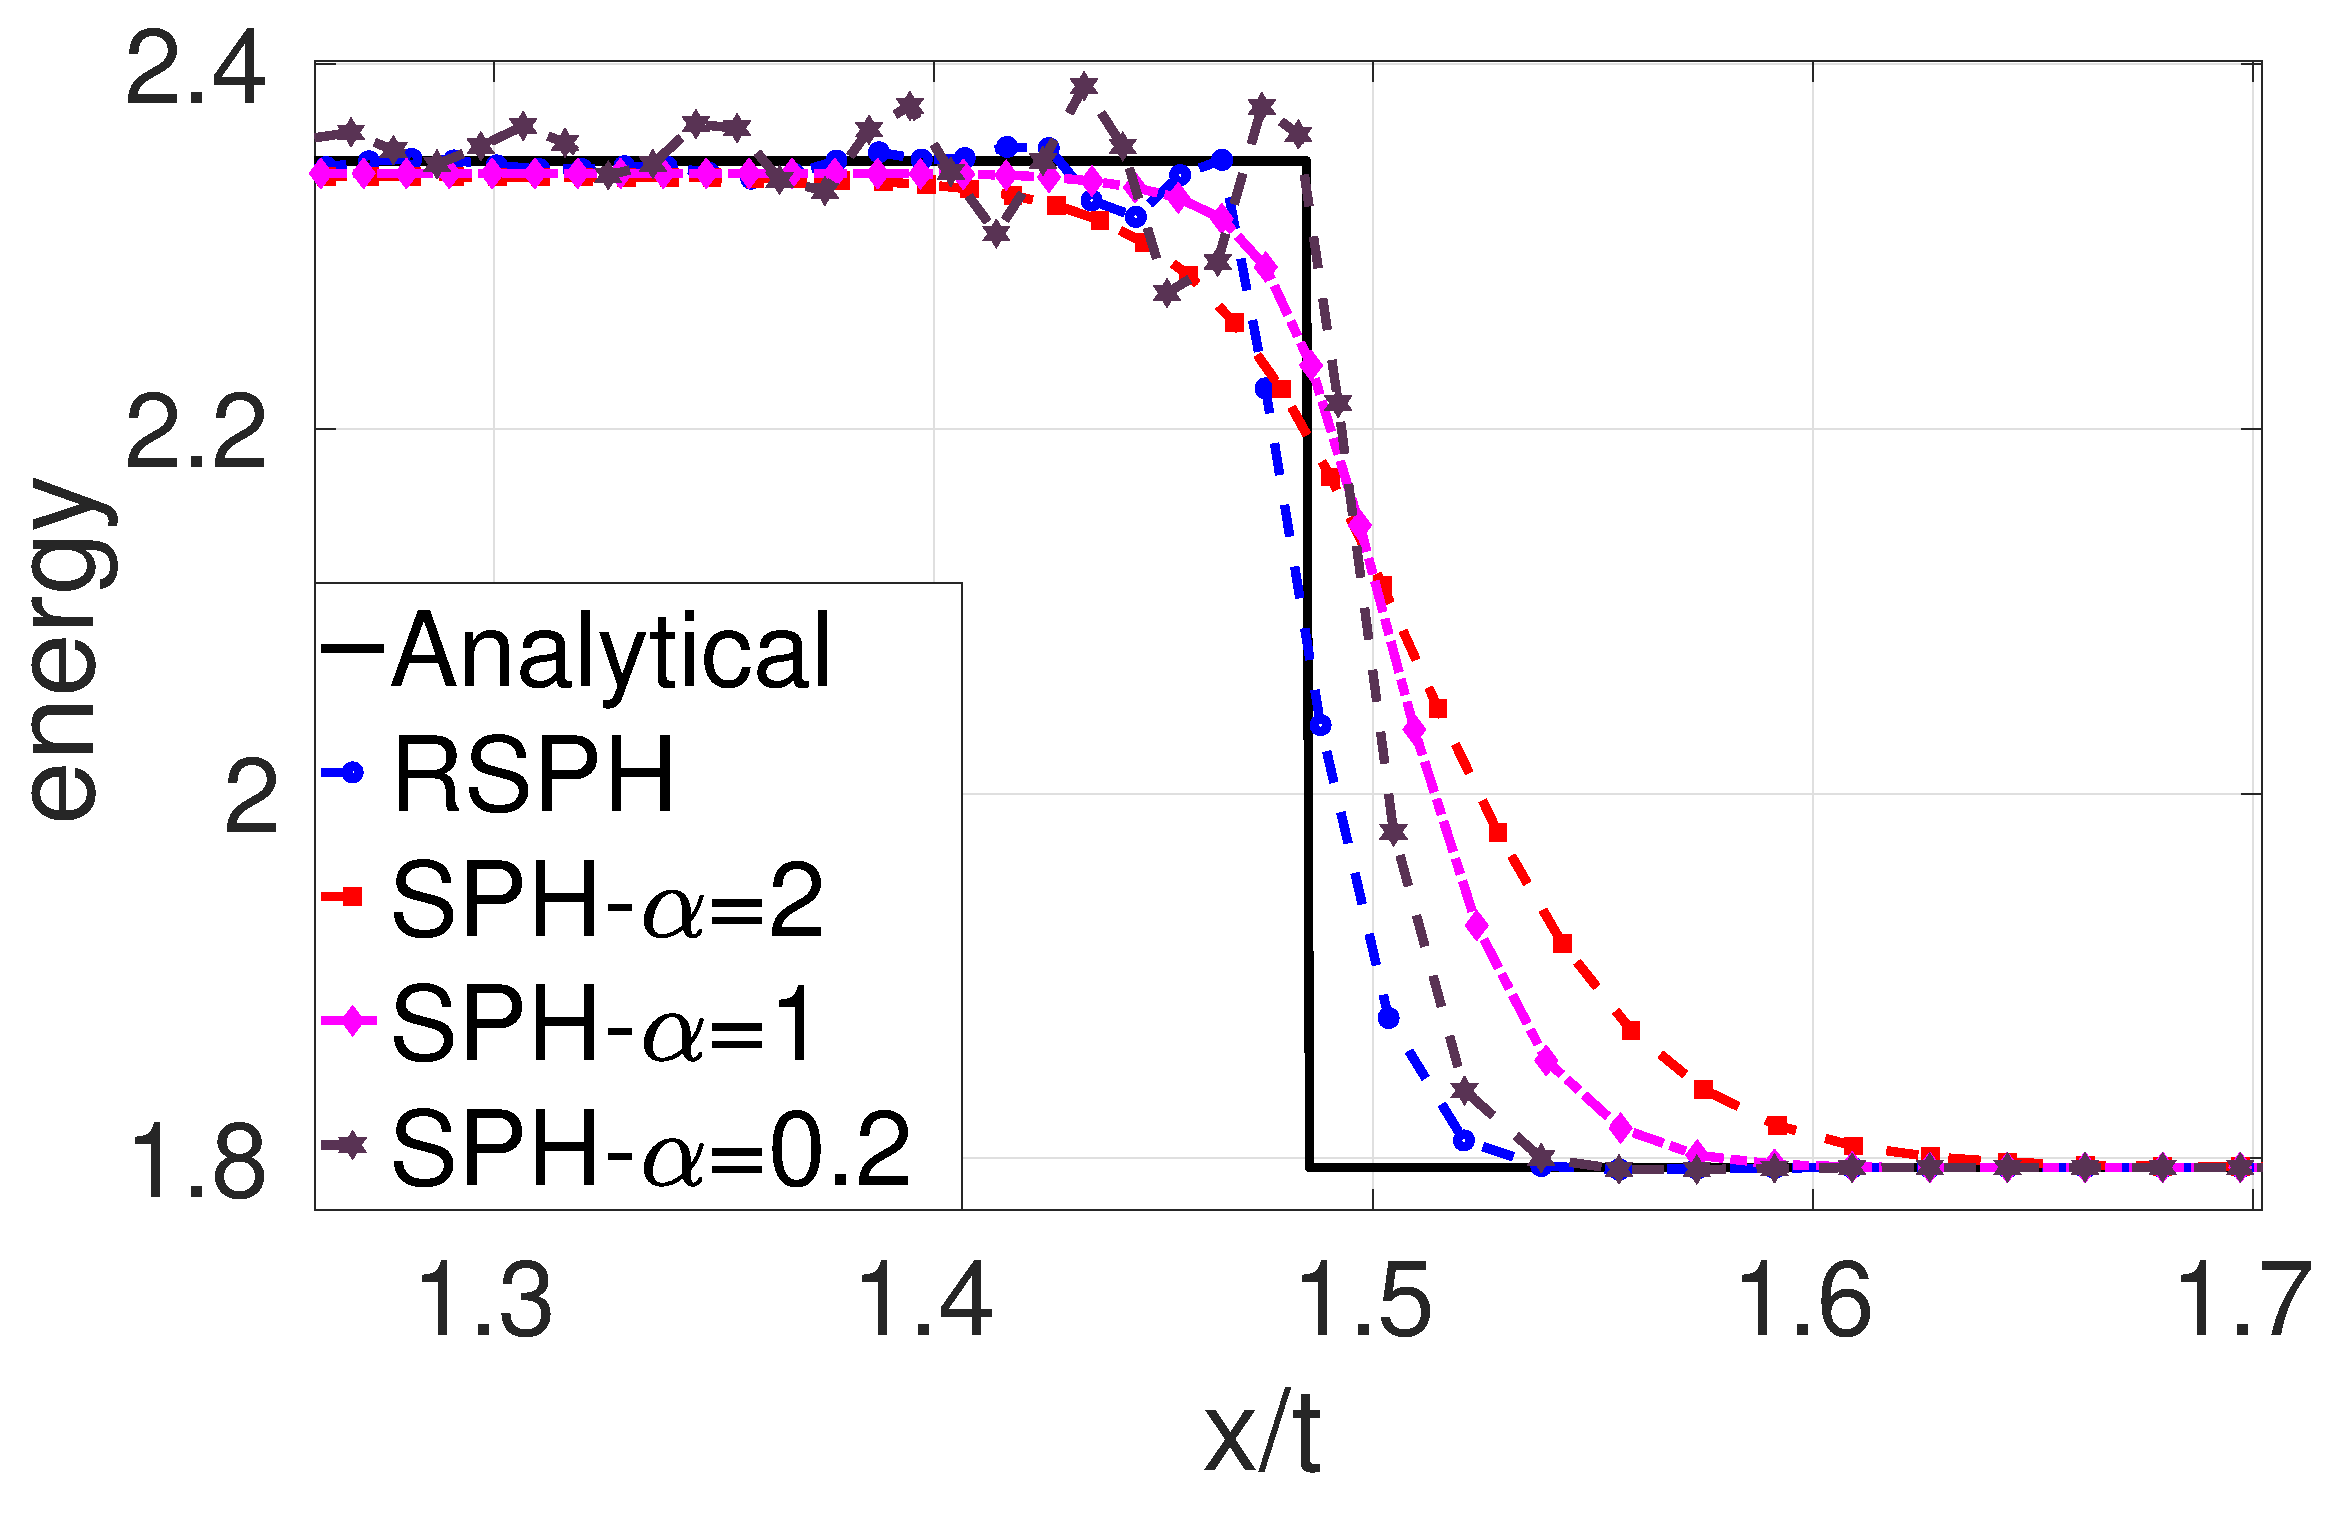
\includegraphics[width=0.99 \textwidth]{./Chapter-4/Figures/Sod/RCM-Sod-SPH-alf-e-zoom}
    \end{minipage}% 
    \begin{minipage}{.33\textwidth}
        \centering
        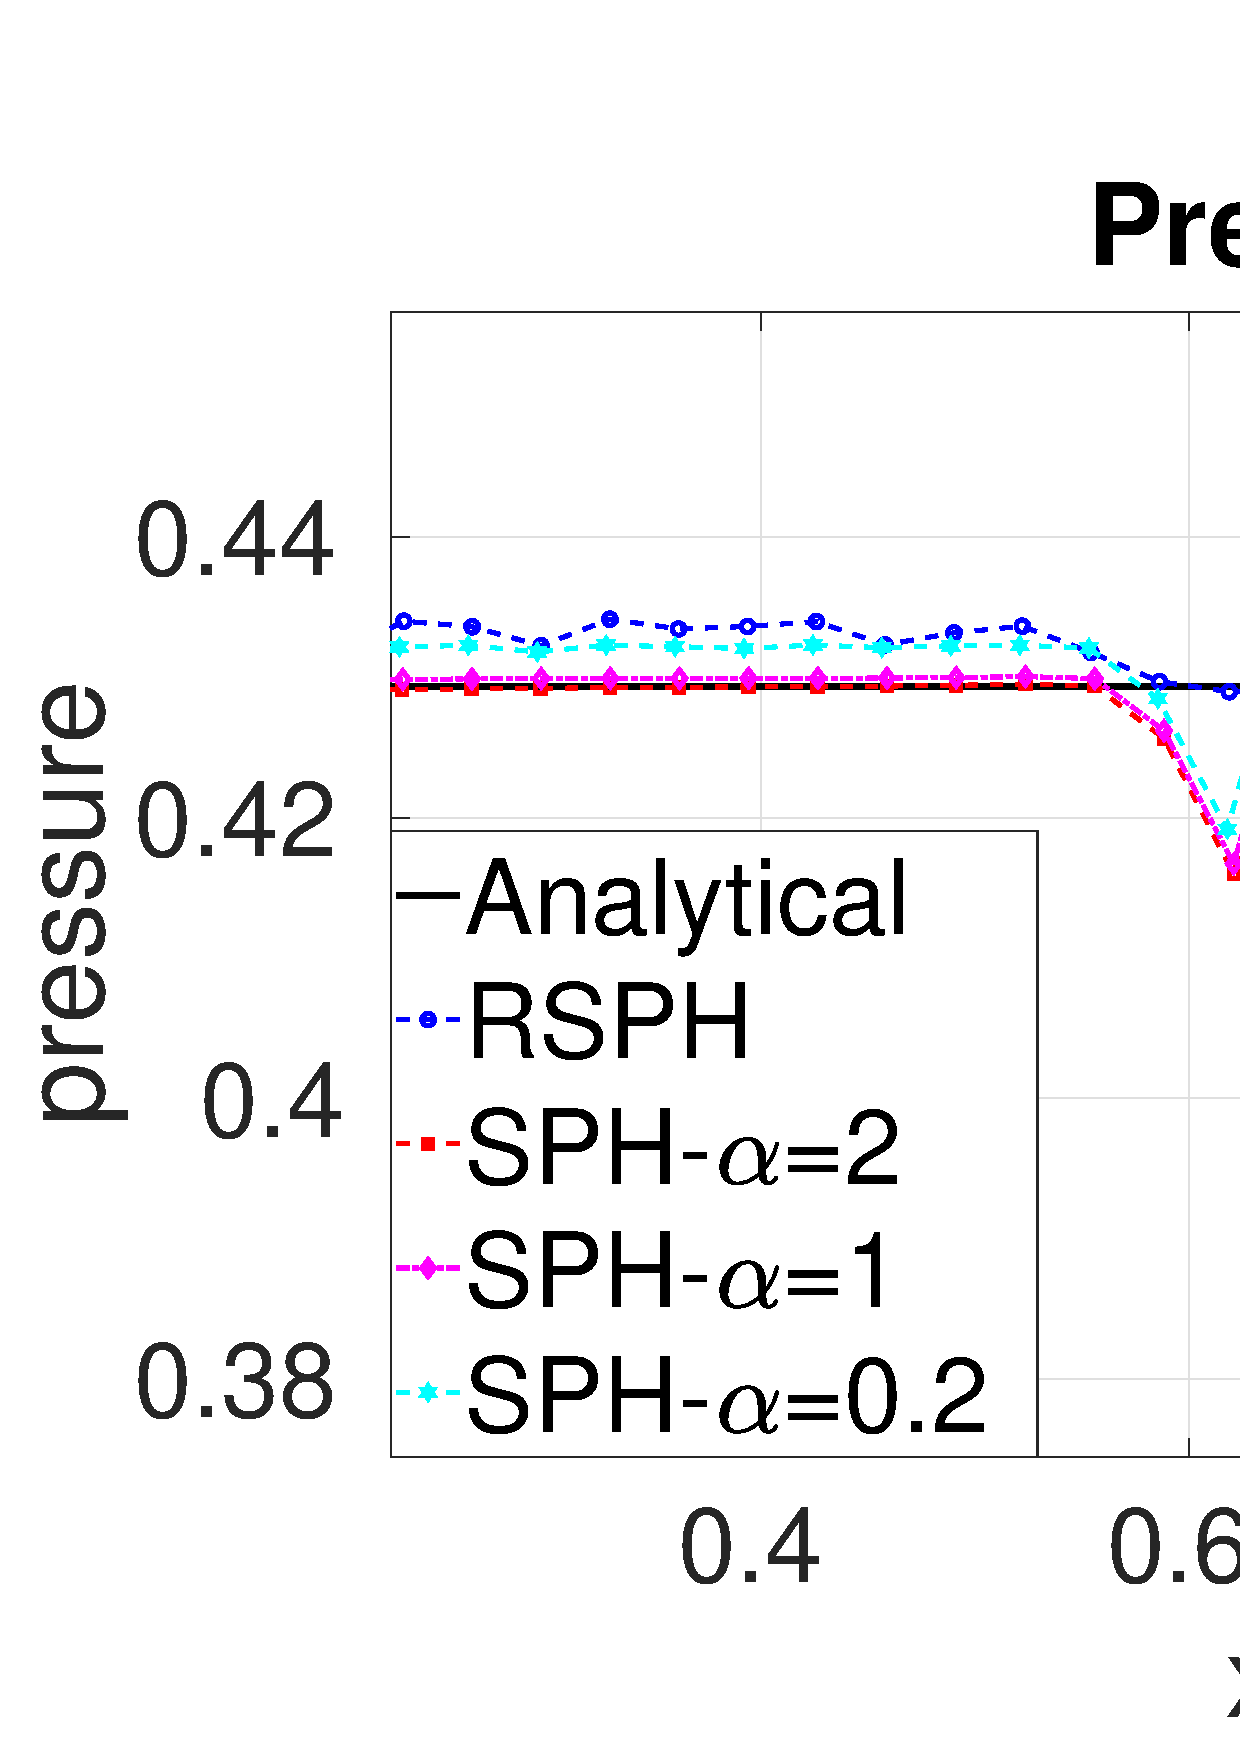
\includegraphics[width=0.99 \textwidth]{./Chapter-4/Figures/Sod/RCM-Sod-SPH-alf-p-zoom}
    \end{minipage}%    
\end{figure}

\begin{minipage}{0.35 \textwidth}
%\begin{figure}[t]
		\centering
        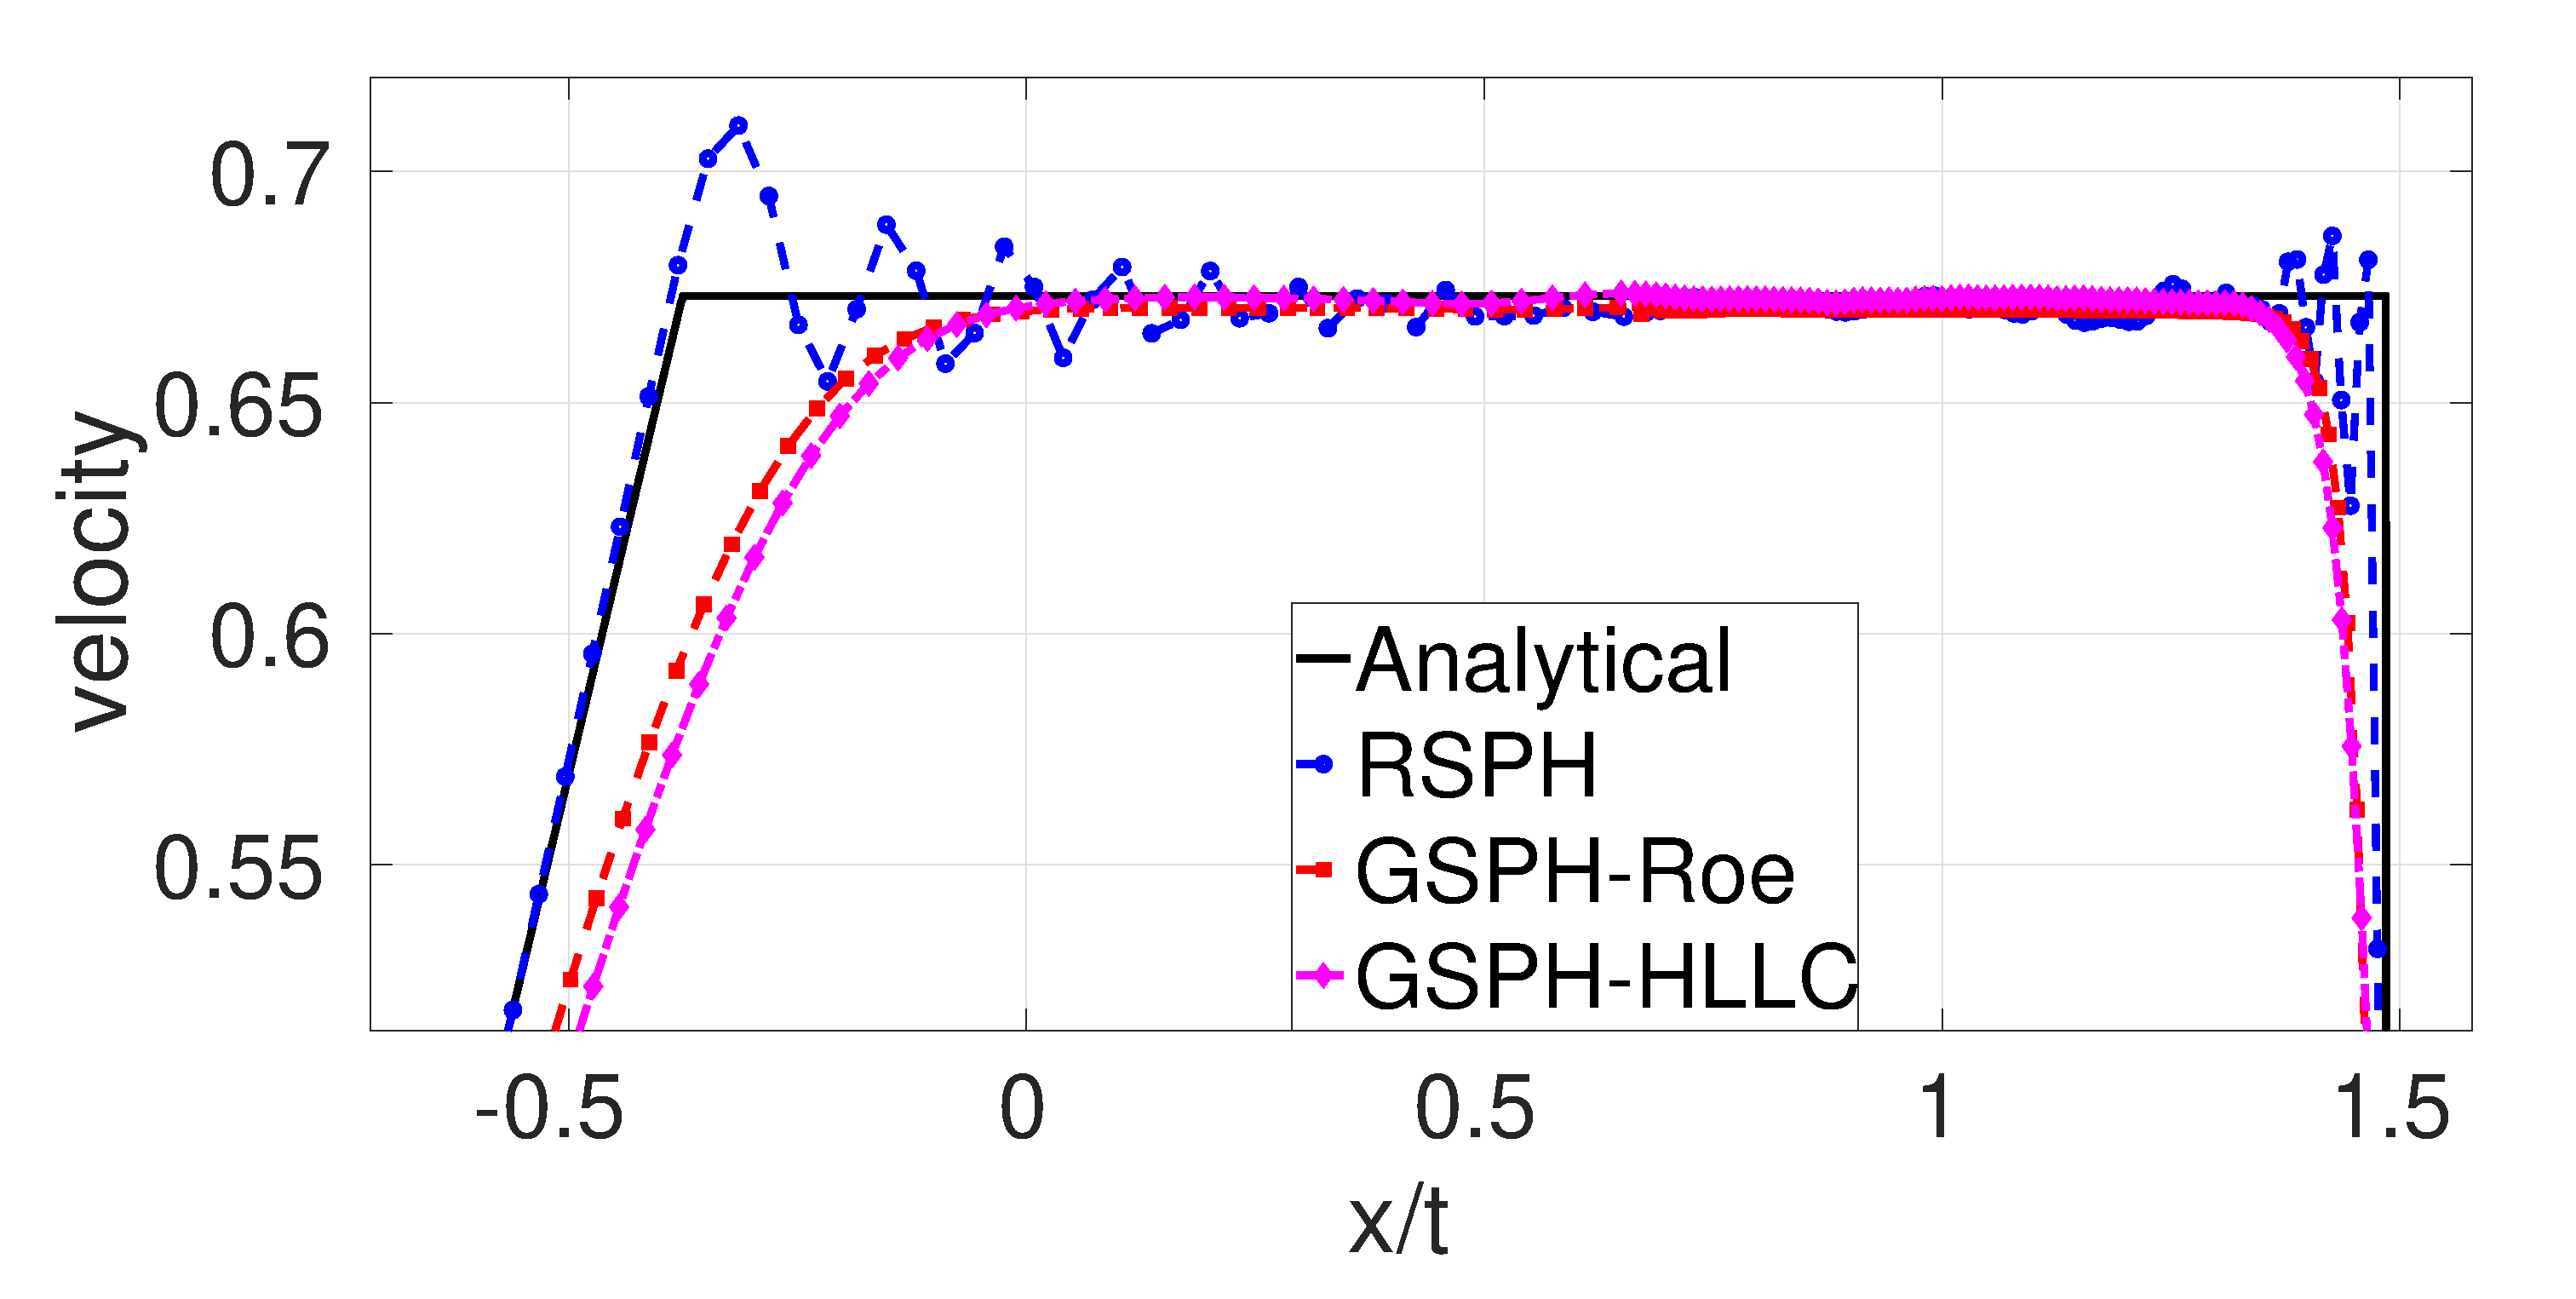
\includegraphics[width=0.99 \textwidth]{./Chapter-4/Figures/Sod/RCM-Sod-GSPH-compare-v-zoom}   
        
        \centering
        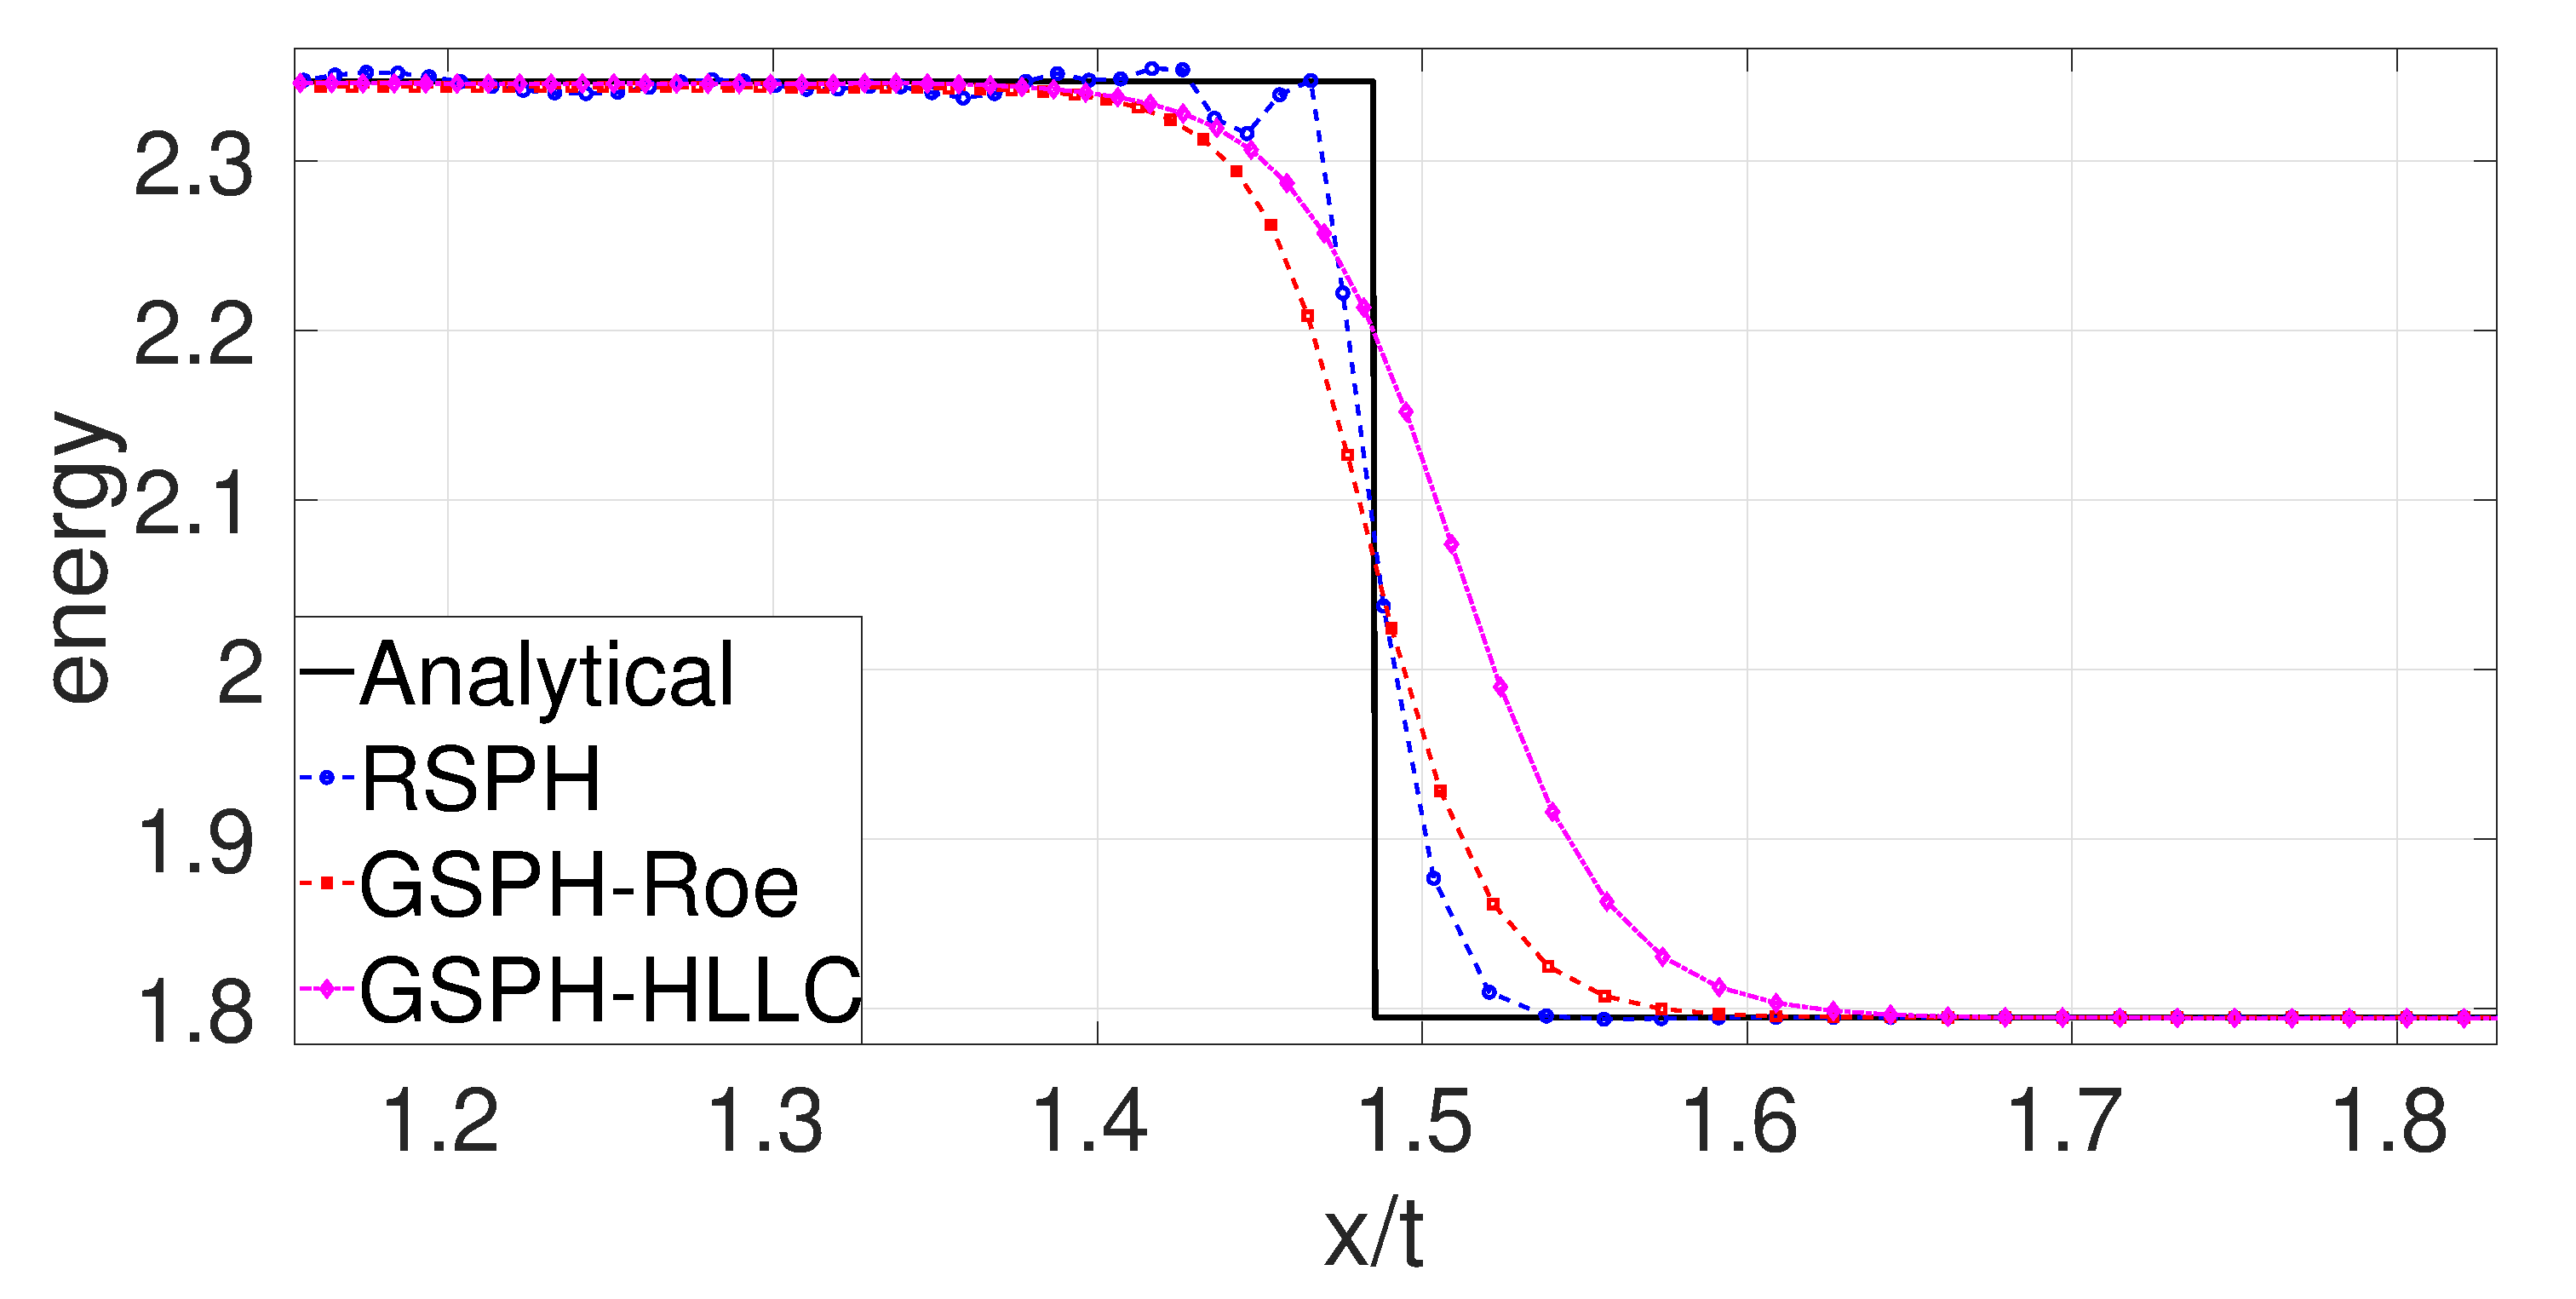
\includegraphics[width=0.99 \textwidth]{./Chapter-4/Figures/Sod/RCM-Sod-GSPH-compare-e-zoom}
%\end{figure}
\end{minipage}
%
\begin{minipage}{0.64 \textwidth}
	\begin{minipage}[b][][b]{.49 \textwidth}
       \centering \small{GSPH}
        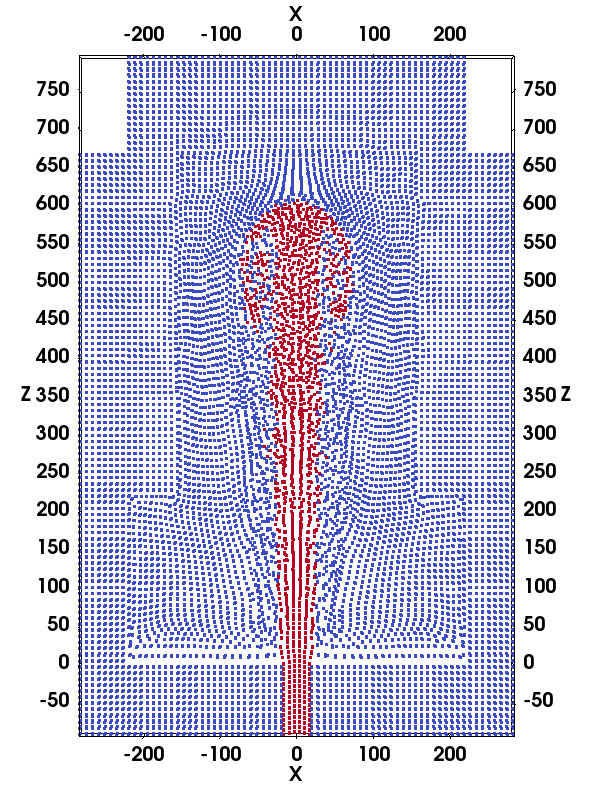
\includegraphics[width=0.99 \textwidth]{./Chapter-4/Figures/GSPH-HLLC-t3-cutView}
    \end{minipage}%
    \centering
    \begin{minipage}[b][][b]{.49 \textwidth}
        \centering \small{RSPH}
        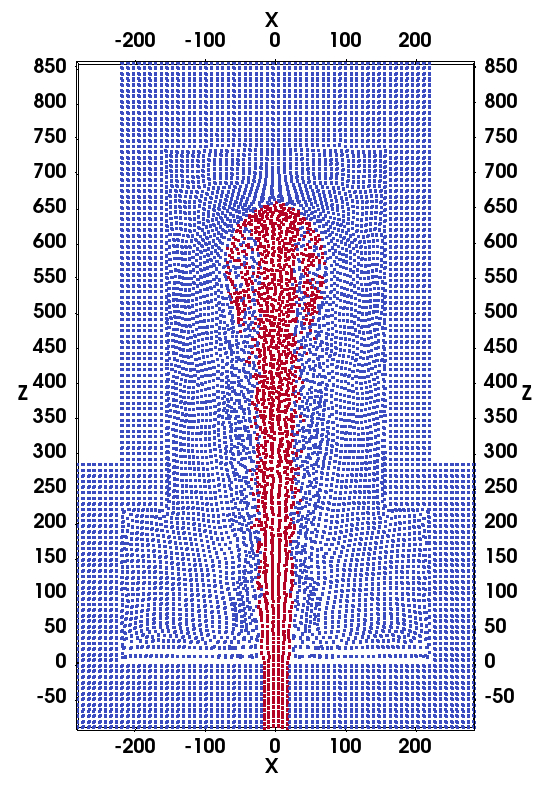
\includegraphics[width=0.99 \textwidth]{./Chapter-4/Figures/RSPH-t3-cutView}
    \end{minipage}%
\end{minipage} 
\end{frame}

\begin{frame}{Discretized Governing Equations}
\begin{equation}
\begin{split}
\left\langle\dfrac{d \textbf{v}_{\alpha}}{d t}\right\rangle 
& =-\sum_b \left[ m_b \left(\dfrac{p_b}{\rho_b^2} + \dfrac{p_{\alpha}}{\rho_{\alpha}^2} + \Pi_{\alpha b}^{\beta} - \Phi_{\alpha b}\right) \bigtriangledown_{\alpha}w_{\alpha b}\left(h\right)\right] \\
& -\sum_j \left[m_j \left(\dfrac{p_j}{\rho_j^2} + \dfrac{p_{\alpha}}{\rho_{\alpha}^2} + \Pi_{\alpha j}^{\beta} - \Phi_{\alpha j}\right) \bigtriangledown_{\alpha}w_{\alpha j}\left(h\right)\right]
+\textbf{g}
\end{split}
\label{eq:gov-sph-v}
\end{equation}
\begin{equation}
\begin{split}
\left\langle\dfrac{d e_{\alpha}}{d t}\right\rangle
& = 0.5\sum_b \left[m_b \widehat{\textbf{v}_{\alpha b}}\left(\dfrac{p_b}{\rho_b^2} + \dfrac{p_{\alpha}}{\rho_{\alpha}^2} + \Pi_{\alpha b}^{\beta} - \Phi_{\alpha b}\right) \bigtriangledown_{\alpha}w_{\alpha b}\left(h\right)\right] \\
& + 2 \sum_b \dfrac{m_b}{\rho_{\alpha} \rho_b} \kappa_{t,\alpha b} \left(T_{\alpha} - T_b\right) F_{\alpha b} \left(h\right) \\
& +0.5\sum_j \left[m_j \widehat{\textbf{v}_{\alpha b}}\left(\dfrac{p_j}{\rho_j^2} + \dfrac{p_{\alpha}}{\rho_{\alpha}^2} + \Pi_{\alpha j}^{\beta} - \Phi_{\alpha j}\right) \bigtriangledown_{\alpha}w_{\alpha j}\left(h\right)\right] \\
& + 2 \sum_j \dfrac{m_j}{\rho_{\alpha} \rho_j} \kappa_{t,\alpha j} \left(T_{\alpha} - T_j\right) F_{\alpha j} \left(h\right)
\end{split}
\label{eq:gov-sph-e}
\end{equation}
\end{frame}

\begin{frame}{Boundary Conditions}
\noindent
\begin{minipage}{0.69 \textwidth}
\begin{figure}
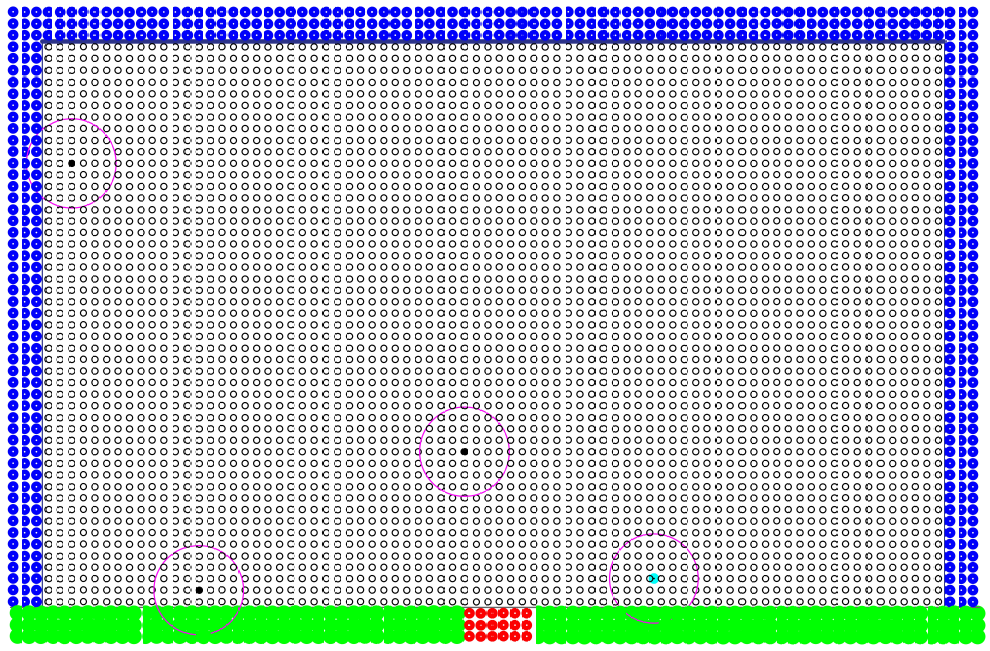
\includegraphics[width=0.99 \textwidth]{./PPT/BC_shot}
\end{figure}
\end{minipage}
\begin{minipage}{0.30 \textwidth}
\begin{figure}
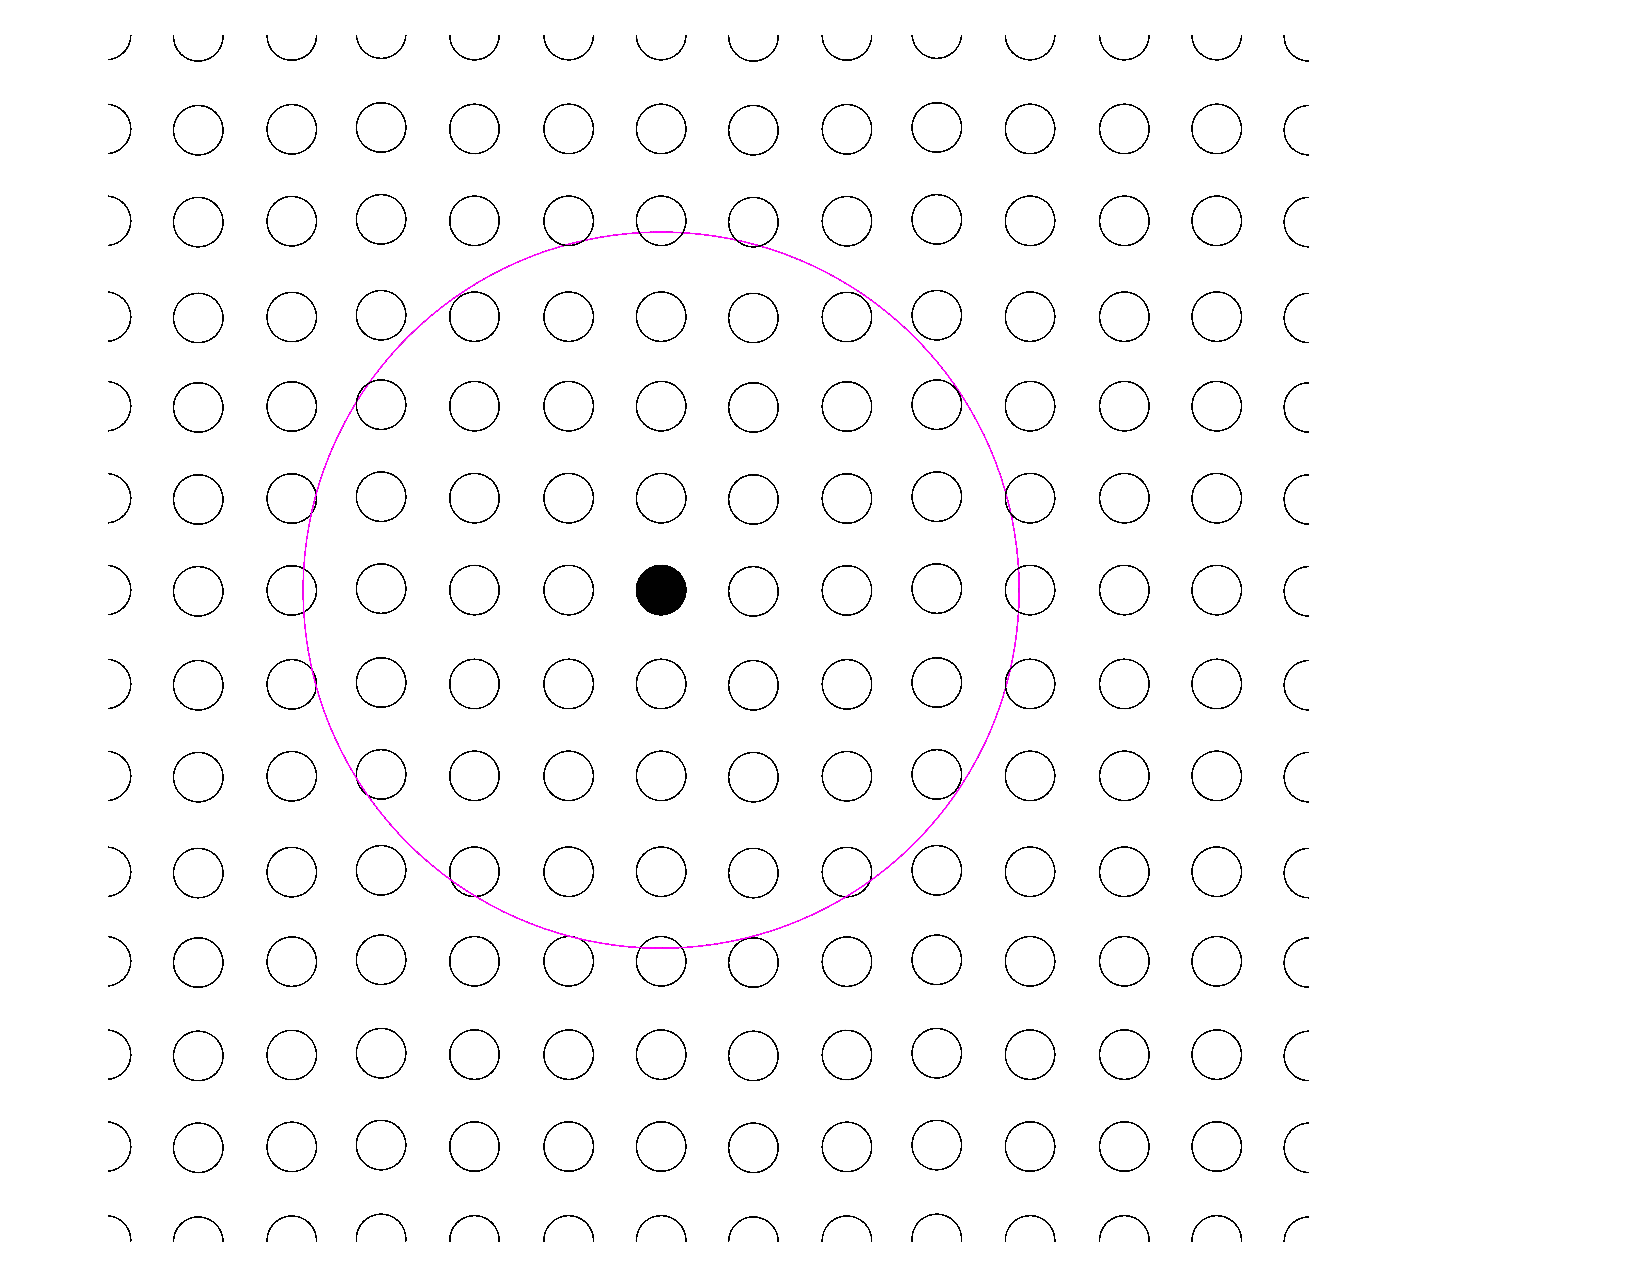
\includegraphics[width=0.99 \textwidth]{./PPT/BC_real}
\end{figure}
\end{minipage}
\\
\begin{minipage}{0.325 \textwidth}
\begin{figure}
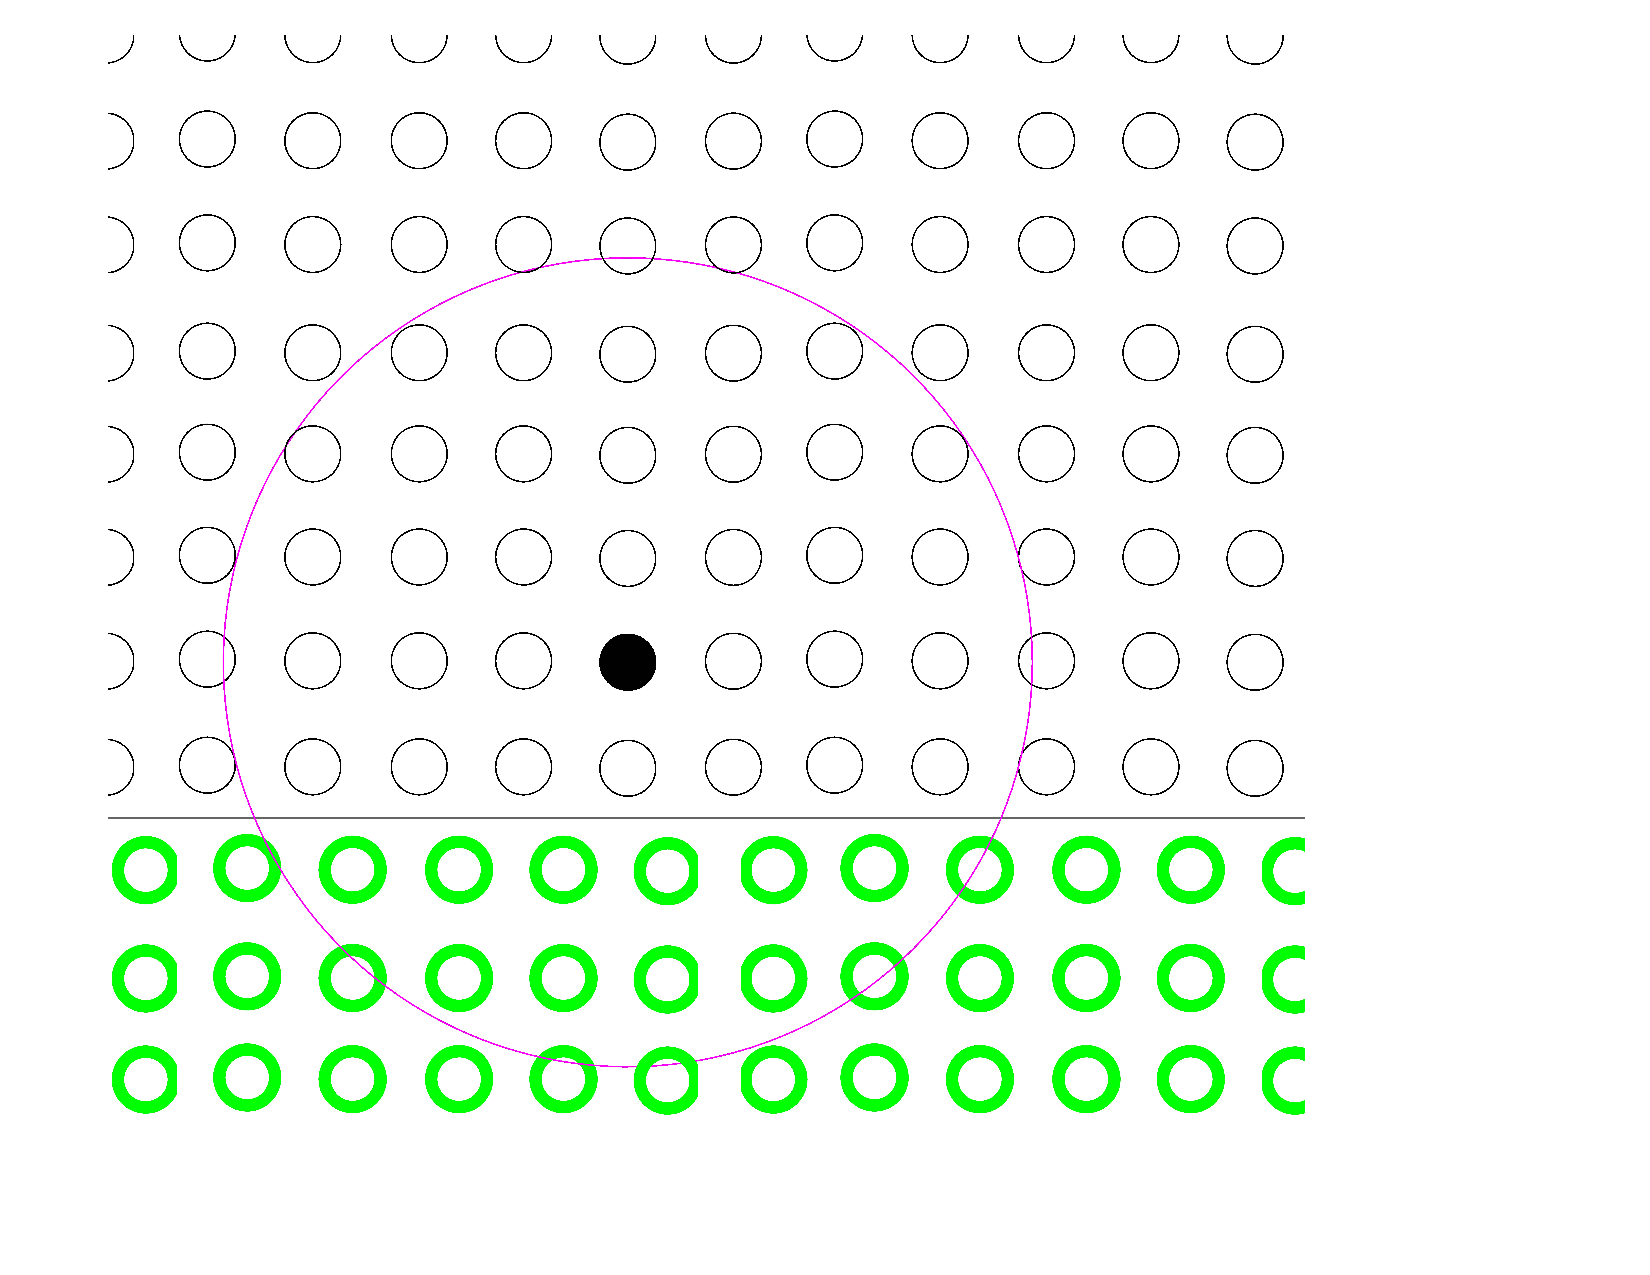
\includegraphics[width=0.99 \textwidth]{./PPT/BC_wall2}
\end{figure}
\end{minipage}
\begin{minipage}{0.325 \textwidth}
\begin{figure}
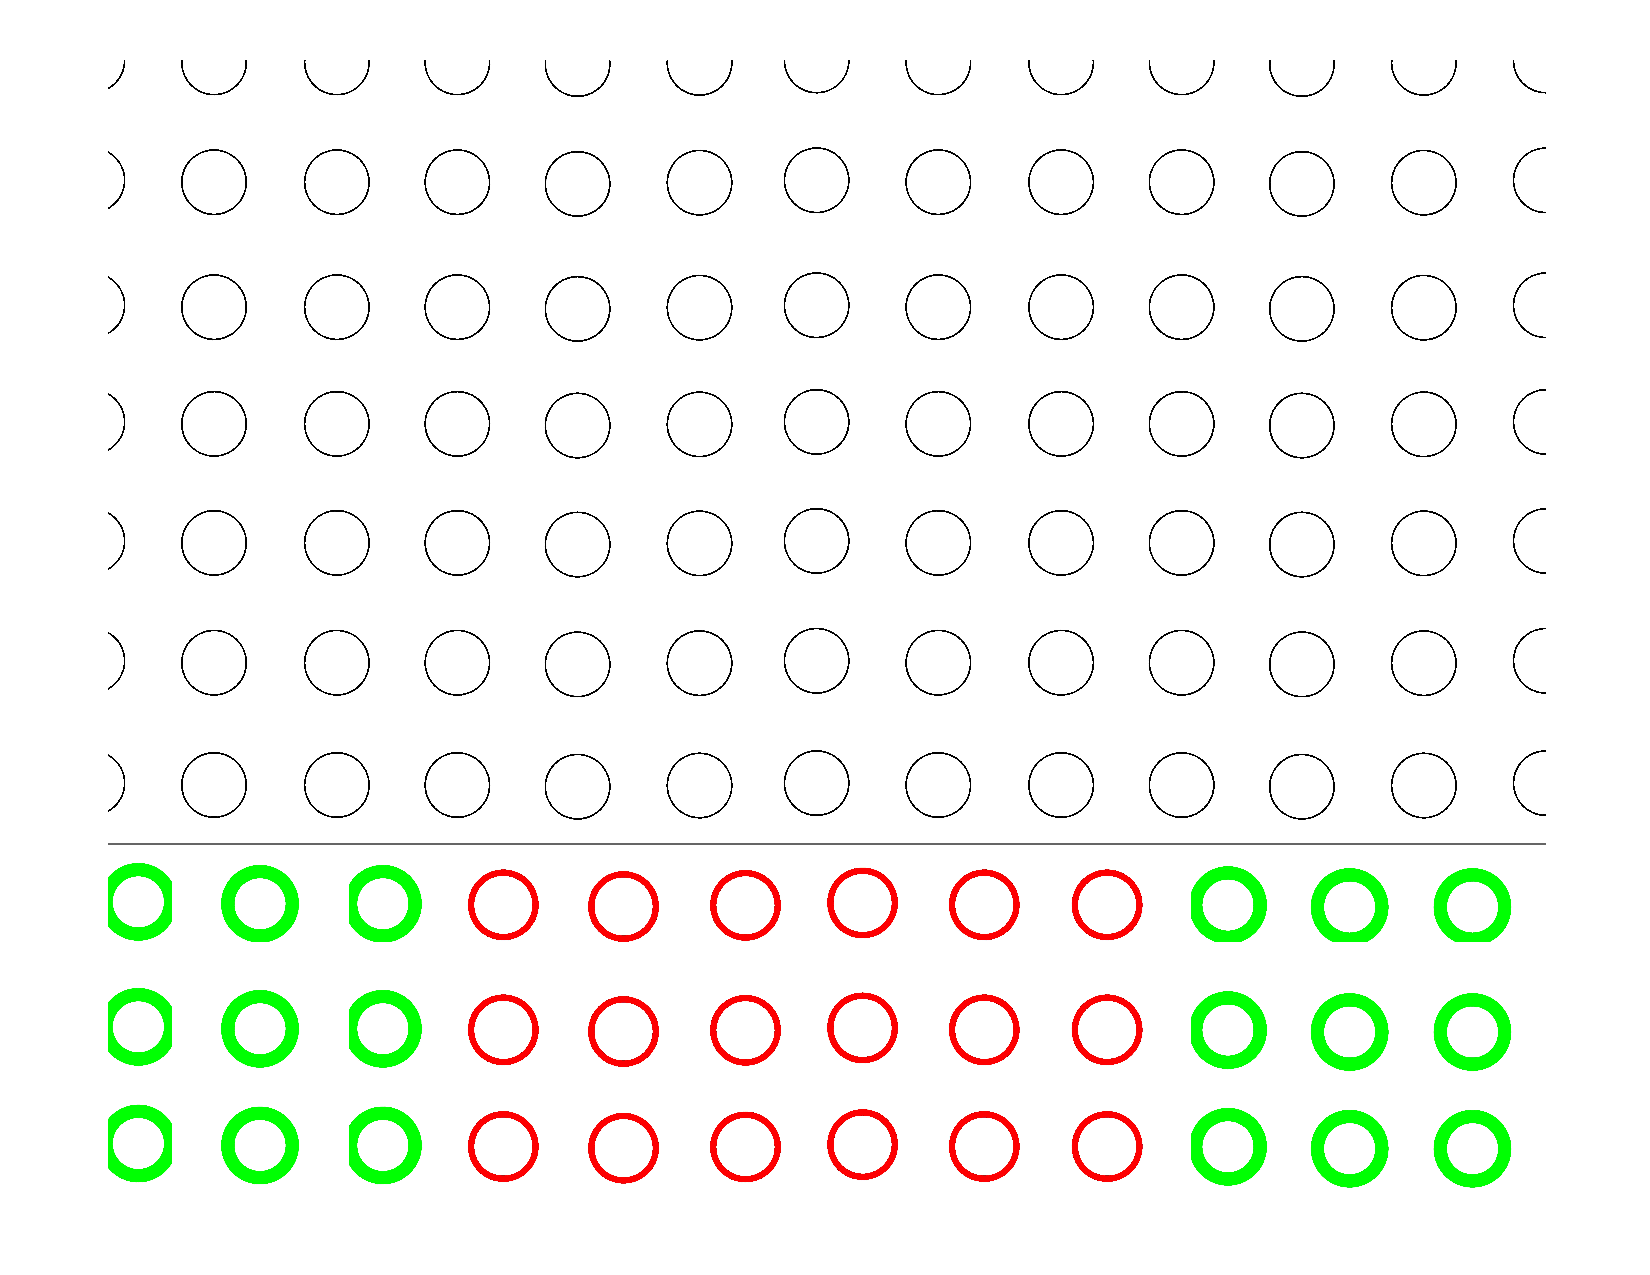
\includegraphics[width=0.95 \textwidth]{./PPT/BC_erupt}
\end{figure}
\end{minipage}
\begin{minipage}{0.325\textwidth}
\begin{figure}
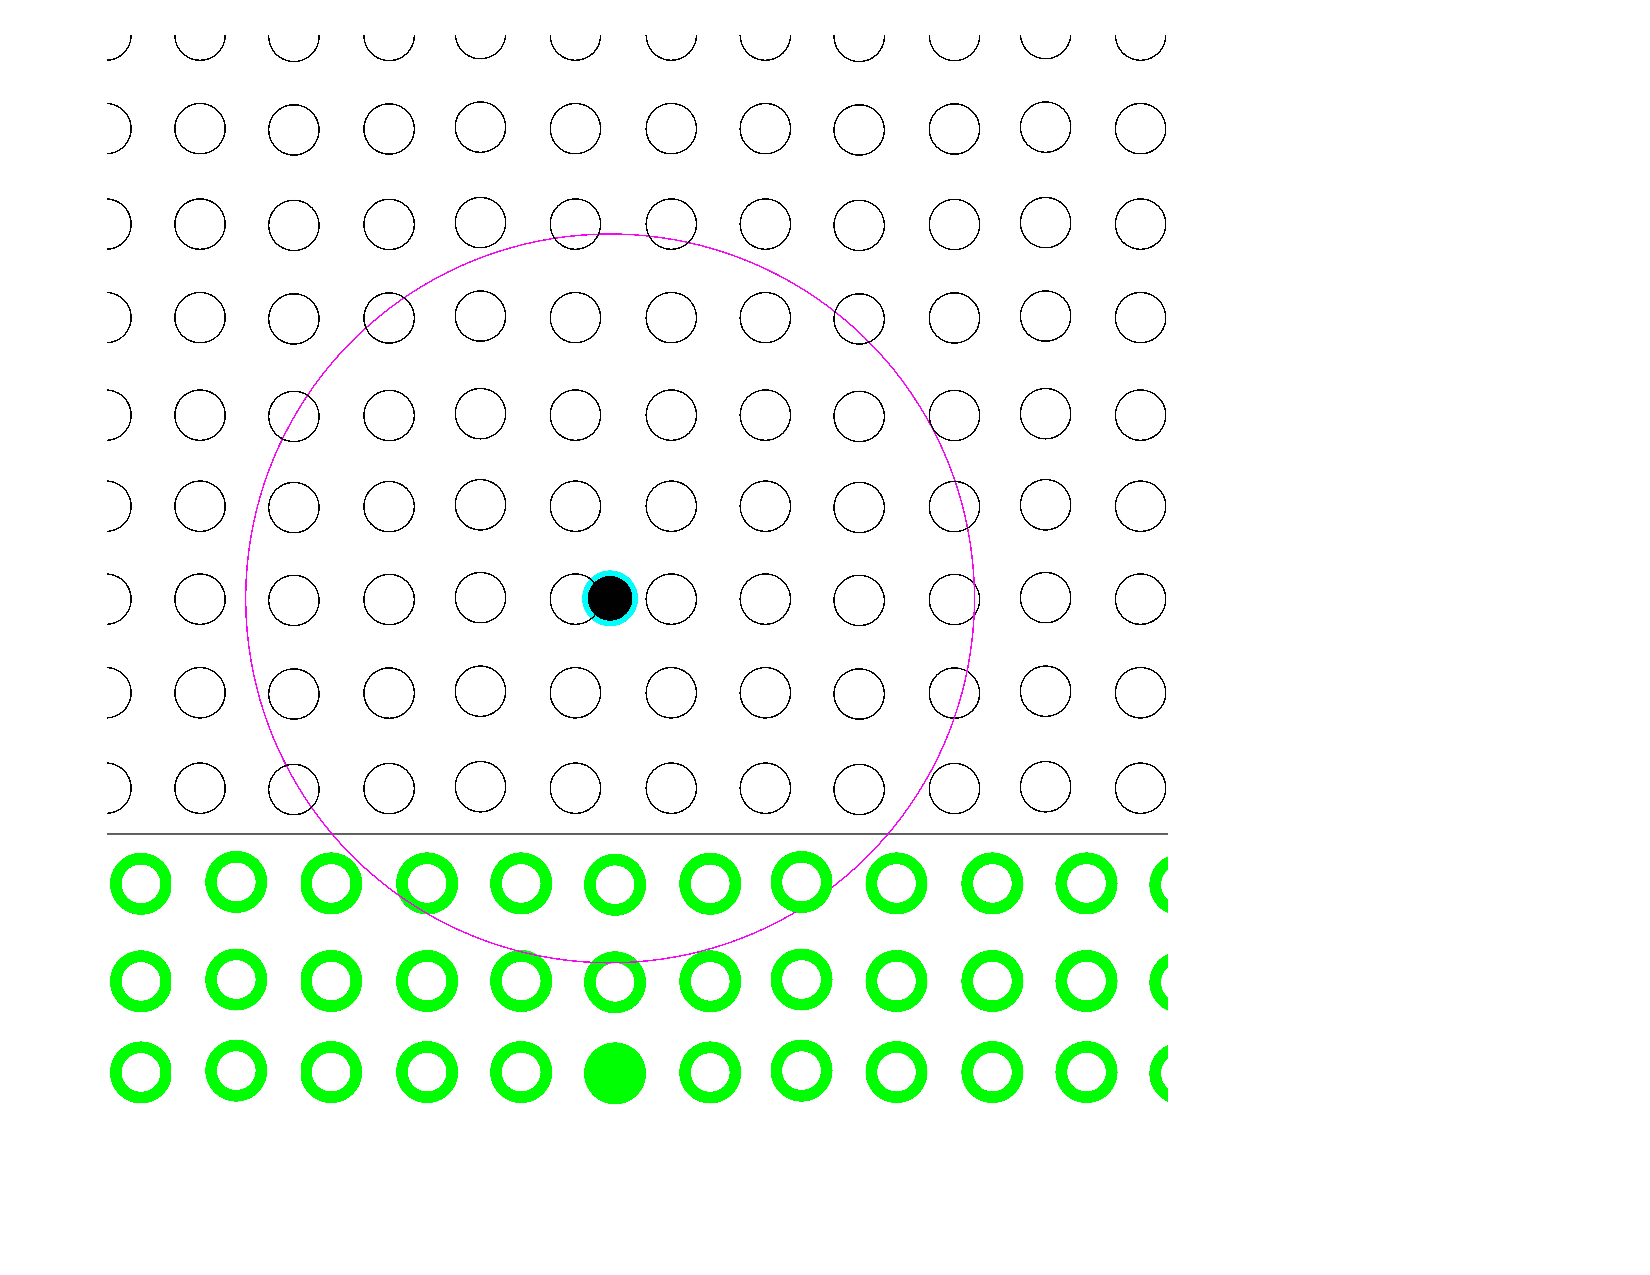
\includegraphics[width=0.99 \textwidth]{./PPT/BC_wall1}
\end{figure}
\end{minipage}
\end{frame}
%------------------------------------------------------------------

%-----------------------------------------------------
\section{Architecture, Data Management and Parallelization}
\begin{frame}{Requirements and Strategies}
All requirements and strategies with respect to code architecture \footcite{cao2017data}.
\begin{figure}[!t]
\centering
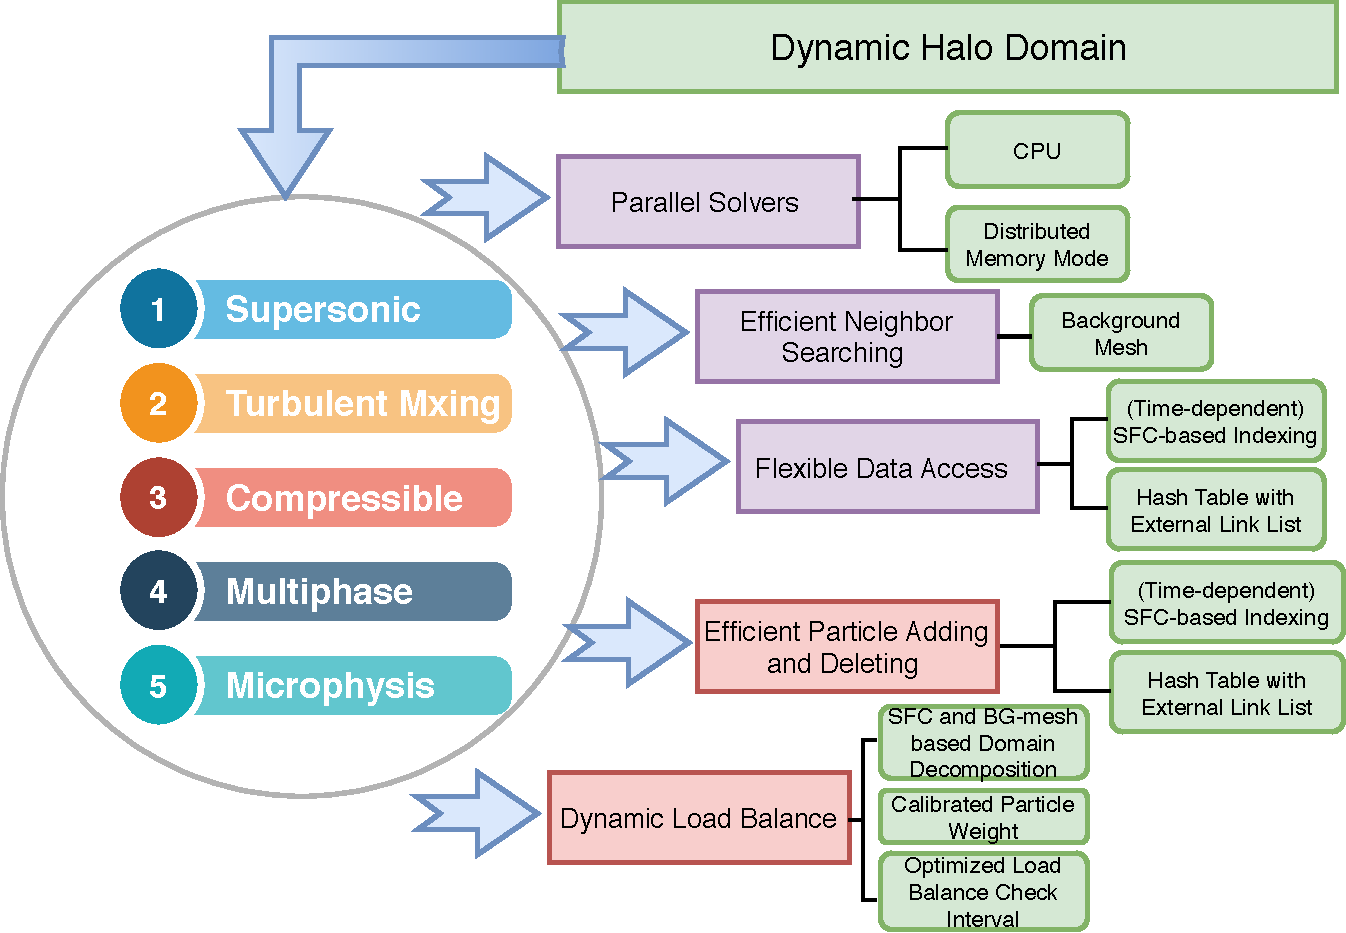
\includegraphics[width=0.83 \textwidth]{./PPT/Requirement_all}
%\caption{Scope of the problem}
\label{fig:Requirements}
\end{figure}
\end{frame}

\begin{frame}{Paricles and Buckets}
\centering
\begin{minipage}{0.66\linewidth}
The basic data structures used to support SPH are particles and buckets %, both are defined as C++ classes
\begin{block}{Particle Class  -- Discretization}
Information that is contained in particle objects :
Unique ID (key), affiliation, {\bf primary variables, secondary variables}, flags and neighbor information.
\end{block}
\begin{block}{Bucket Class -- Partition and neighbour searching}
Information that is contained in bucket objects :
Unique ID (key), affiliation, dimension information, flags, neighbor information and contained particles.
\end{block}
\end{minipage}
\begin{minipage}{0.33 \linewidth}
\begin{figure}
\flushright
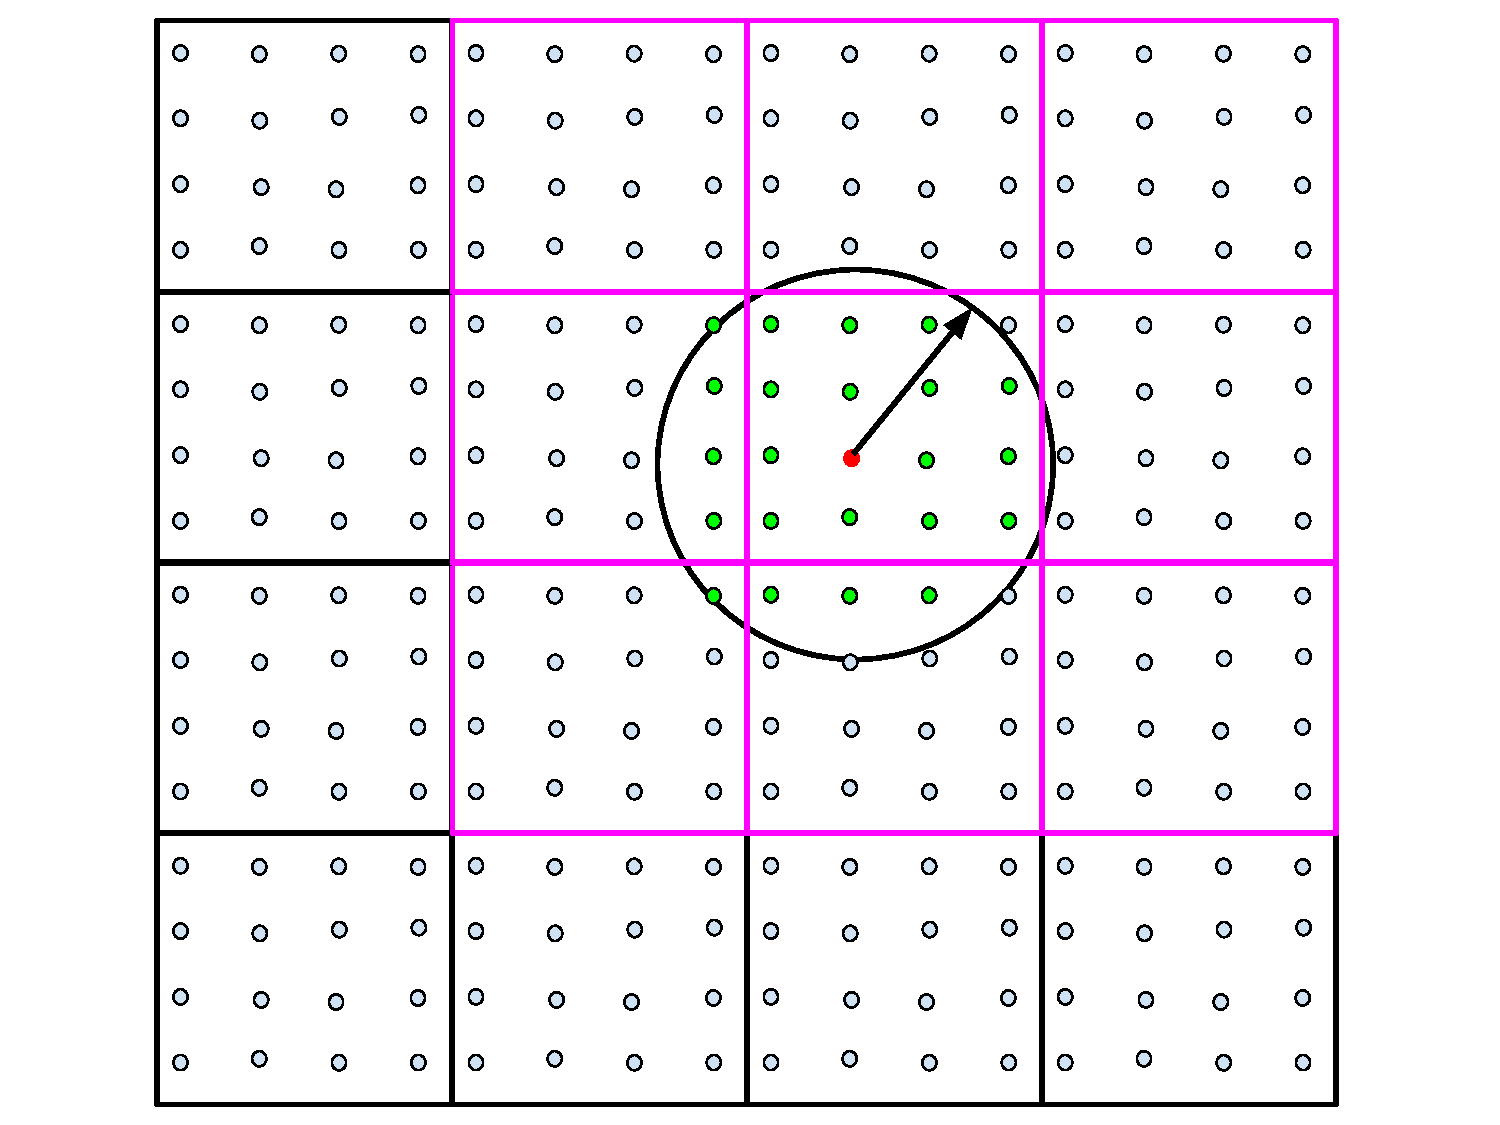
\includegraphics[width=0.75\textwidth]{./PPT/Neighbor-Search}
\\
\flushright
\includegraphics[width=0.75\textwidth]{./Chapter-5/Figures/SFC_particles_buckets}
\\
\flushright
\includegraphics[width=0.70\textwidth]{./Chapter-5/Figures/SFC_particles_buckets_partition}
\end{figure}
\end{minipage}
\end{frame}

\begin{frame}{SFC-based Index}
SFC based key is defined as: $k = h_n (\textbf{x})$, Where $h_n (\textbf{x}): [0,1]^n \rightarrow [0,1]$
\begin{block}{Features of SFC-based Index}
  \begin{itemize}
  \item {
    Guarantee uniqueness of the indexing.
  }
  \item {
    Generating of indices are fast and
independent
  }
  \item {
    Conserve spatial locality in ordering $\rightarrow$ promotes memory locality / {\bf cache reuse}
  }
  \item {
    Global address space and ordering for use in  domain decomposition
  }
  \end{itemize}
\end{block}

\begin{block}{Time-dependent SFC}
\begin{equation}
h_n: [0,1]^n \times \textbf{T} \rightarrow [0,1] \times \textbf{N}
\end{equation}
Where $\textbf{T} \subset [0,\infty)$ is the time dimension, and $\textbf{N}=\lbrace 0, 1, 2, 3...\rbrace$. \\
Then the time-dependent key can be expressed as: $(k,n)$
\end{block}
\end{frame}

\begin{frame}{Data management}
\begin{minipage}{0.66 \textwidth}
\begin{figure}
\includegraphics[width=0.95\textwidth]{./Chapter-5/Figures/Particle_adding_with_link}
\end{figure}
\end{minipage}
\begin{minipage}{0.33 \textwidth} 
\small
Time complexity: 

\begin{itemize}
\item Hashtable: $O(1)$
\item Array: $O(1)$ add, delete not allow
\item List: $O(N)$
\item Vector: $O(1)$, add, delete expensive
\item Hashmap: $O(logN)$
\end{itemize}

\end{minipage}
\small
\begin{block}{Hash Function}
\begin{equation}
slot= \frac{Key - Min\,Key}{Max\,Key - Min\,Key} 
\times Hash\,Table\,Size 
\label{eq:hash_function}
\end{equation}
To avoid a non-uniform sparse hash table, only plug the first number, $k$, of the key, into Eq. (\ref{eq:hash_function}). All particles with the same birth location will hash to the same index and be handled by external linked lists.
\end{block}
\end{frame}

%\begin{frame}{Load Balance (Naive way)}
%\begin{figure}
%\flushleft
%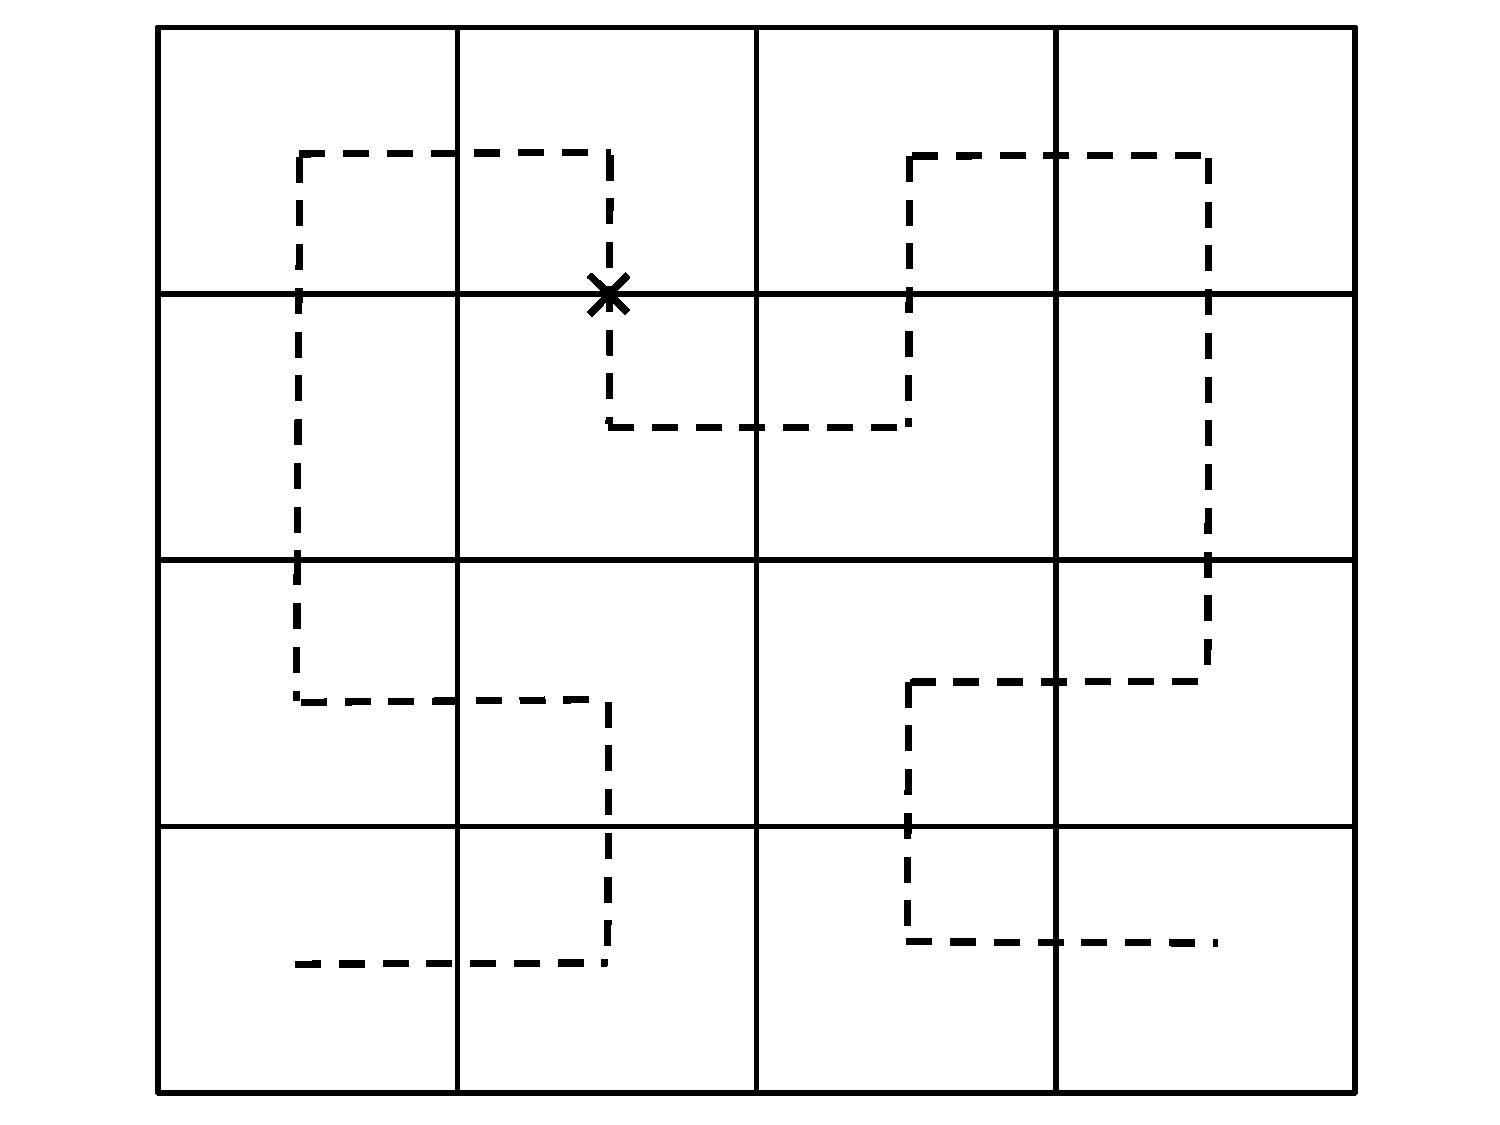
\includegraphics[width=0.3\textwidth]{./PPT/SFC_bucket_decomposition}
%\hfill
%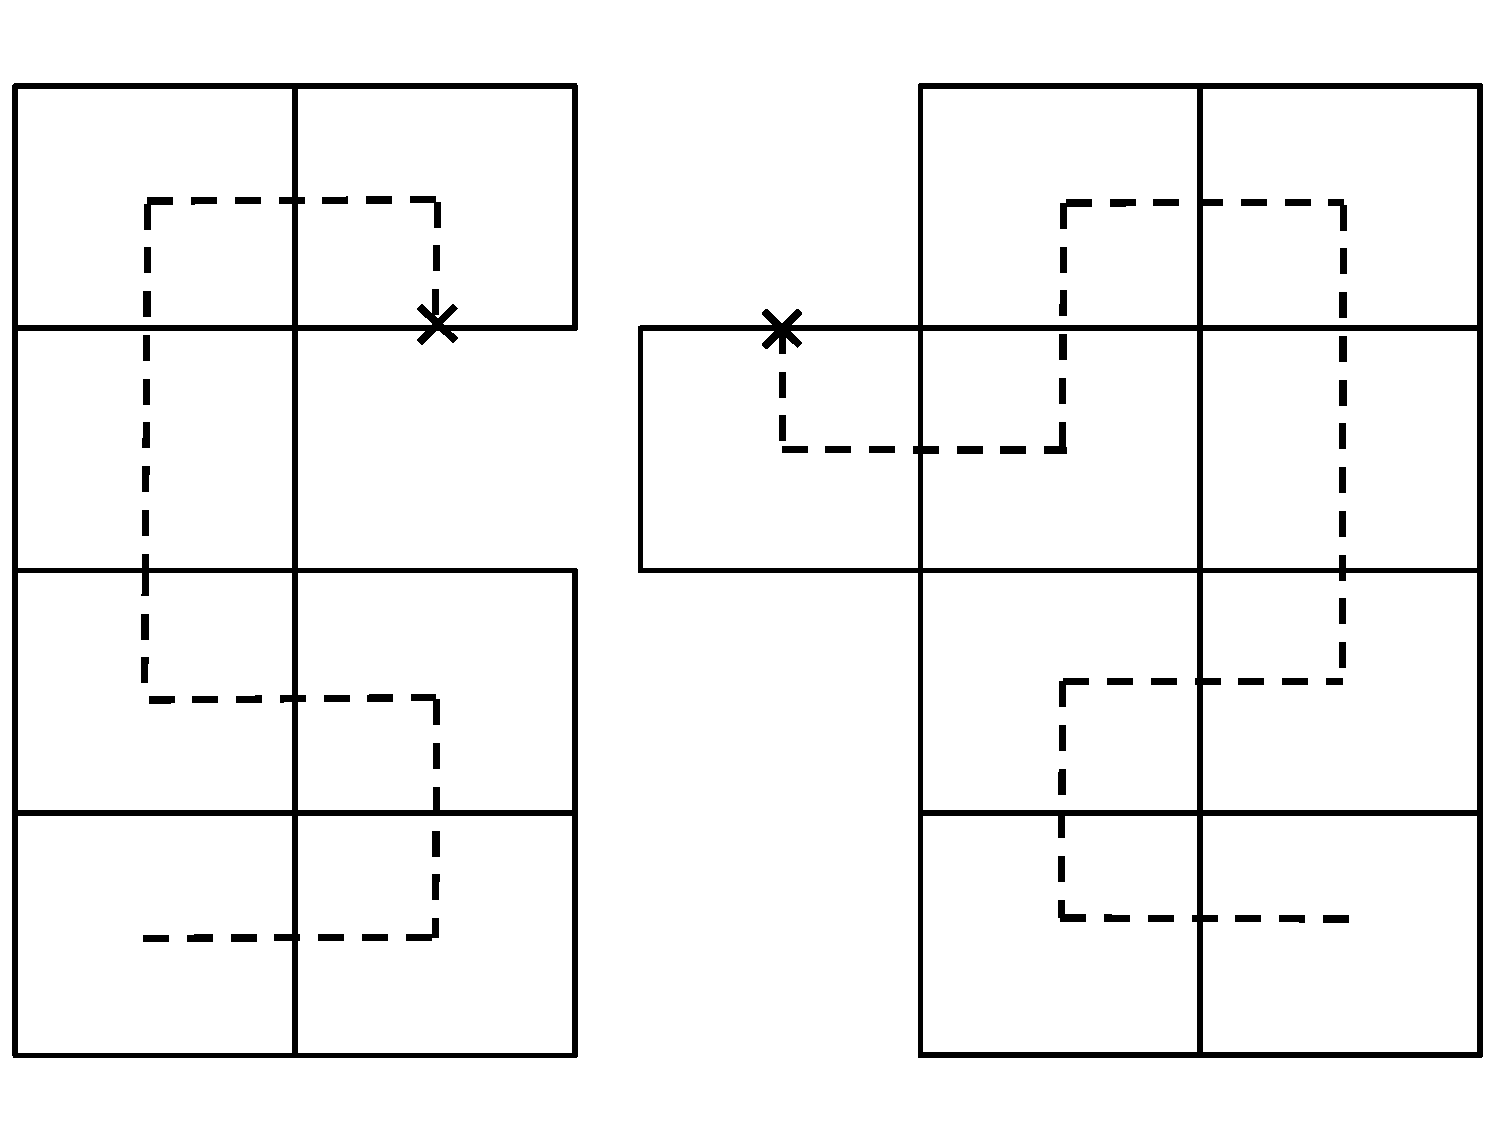
\includegraphics[width=0.305\textwidth]{./PPT/SFC_bucket_decomposition_Partition}
%\end{figure}
%
%\begin{figure}
%\flushleft
%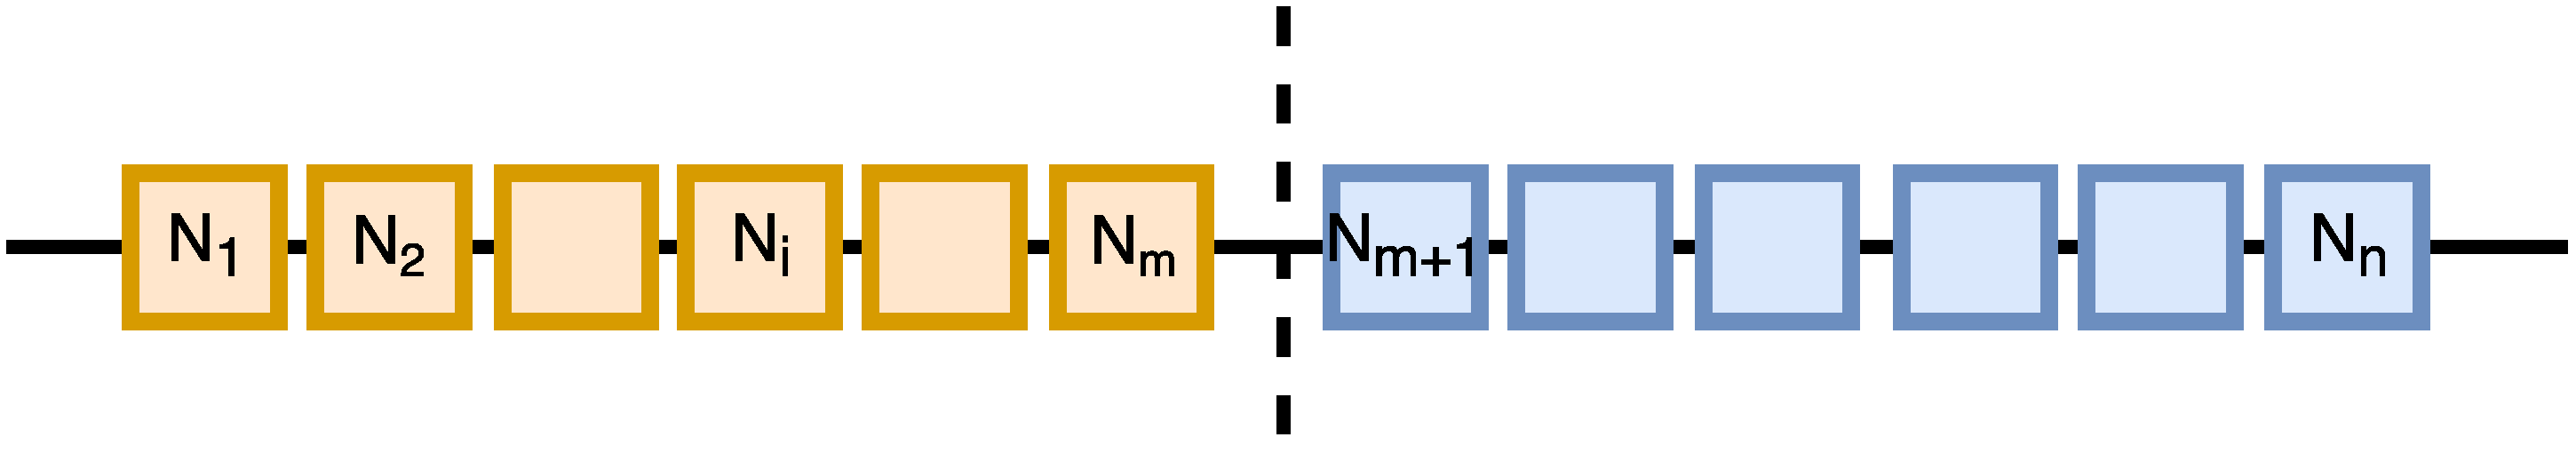
\includegraphics[width=0.93\textwidth]{./PPT/Domain-Decomposition}
%\end{figure}
%
%Where $N_i$ is the total number of particles contained by the $ith$ bucket. $N_i$ can be used to indicate computational workload associated that bucket. 
%
%Cut the SFC into pieces so that workload are splitted alomost equally.
%\begin{equation}
%\sum_{i=1}^{m} N_i \approx \sum_{i=m+1}^{n} N_i
%\end{equation}
%\end{frame}

\begin{frame}{Load Balance (Weighted particles)}
\begin{minipage}{0.3 \textwidth}
\begin{figure}
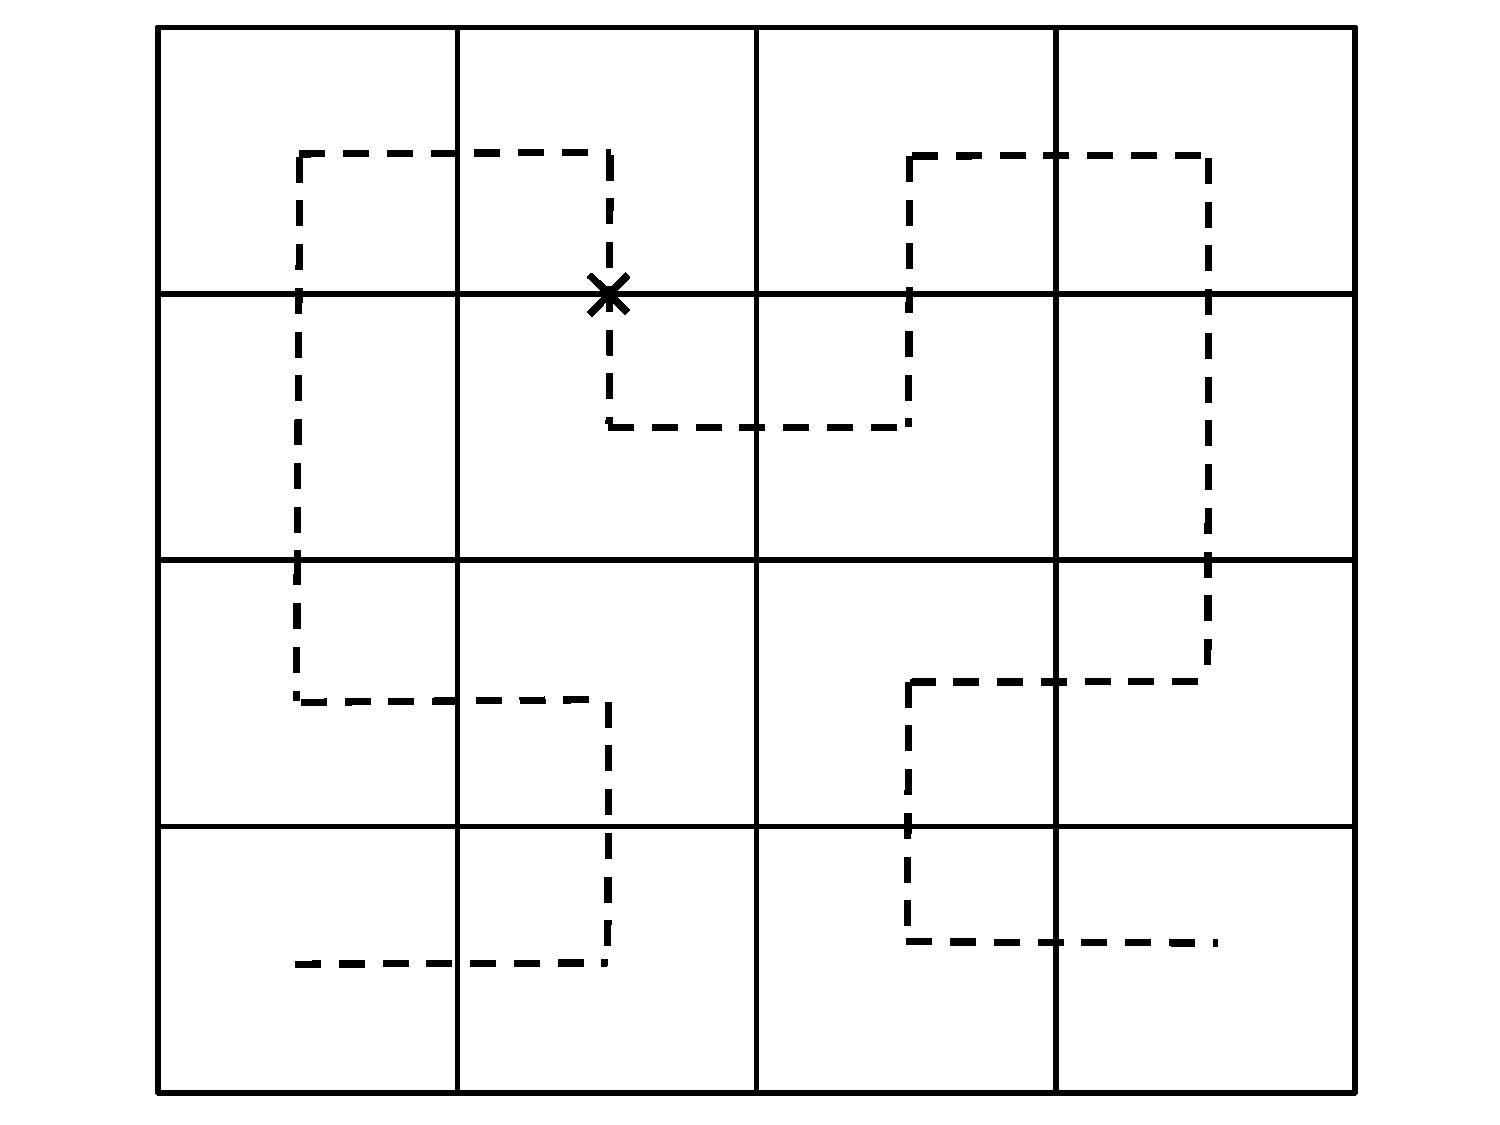
\includegraphics[width=0.99\textwidth]{./PPT/SFC_bucket_decomposition}
\end{figure}
\end{minipage}
\begin{minipage}{0.69 \textwidth}
\begin{figure}
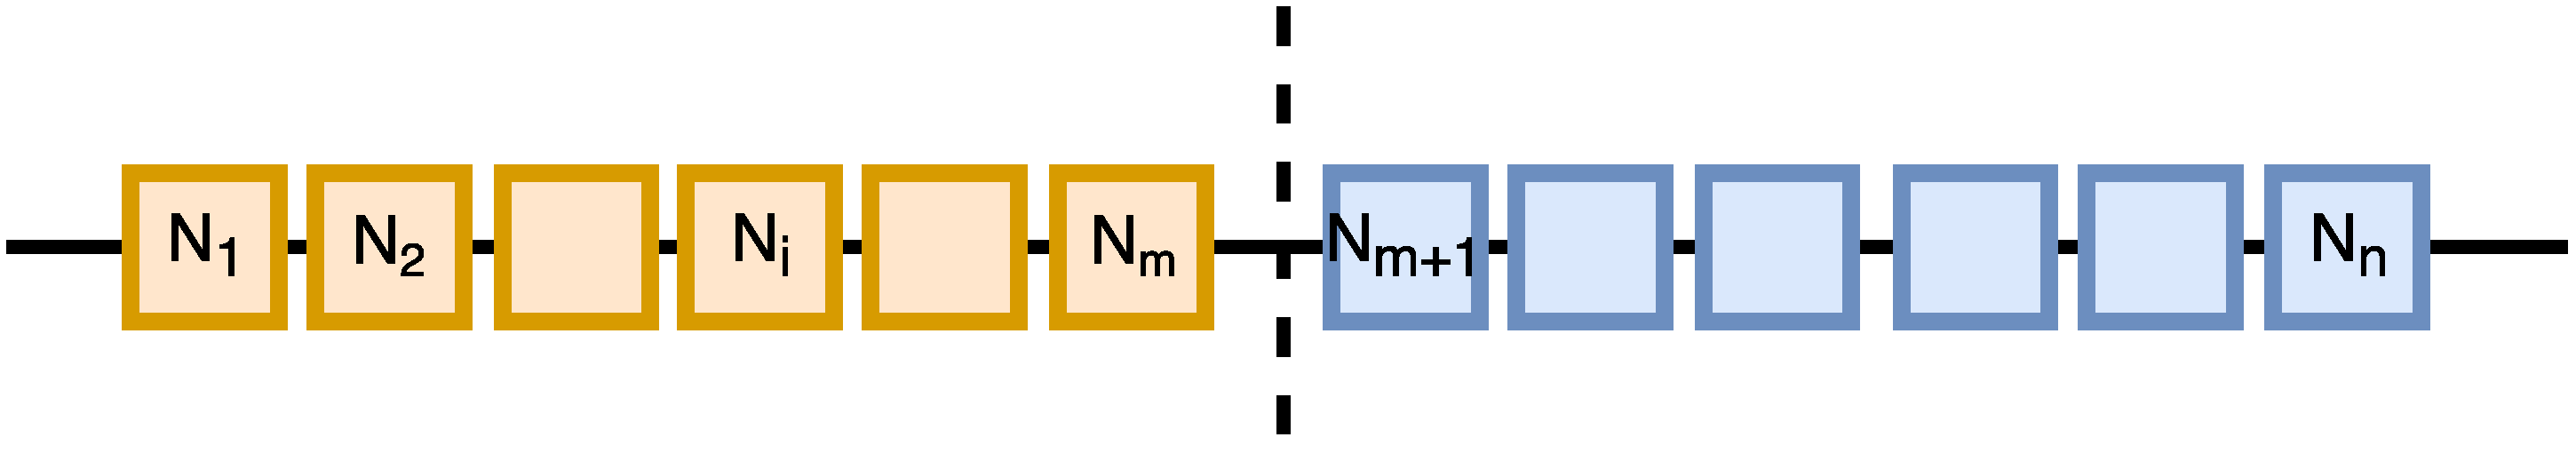
\includegraphics[width=0.99\textwidth]{./PPT/Domain-Decomposition}
\end{figure}
$$
\sum_{i=1}^{m} N_i \approx \sum_{i=m+1}^{n} N_i 
~~~~~
W^{bucket} = \sum_i^{N^{particle}} W_i^{particle}
$$
\end{minipage}

%The domain is decomposed by cutting SFC of buckets into pieces of equal work load. 
%The work load of each bucket can be more precisely calculated by summing up workload of all particles contained in that bucket. 
%The work load associated to each particle is calibrated based on profilling data.
\begin{table}
\resizebox{0.9\textwidth}{!}{  
	  \begin{tabular}{lrrrrrr}
	    \hline
	    Step & Cost ($ms$) & Real & wall & eruption & pressure\\
	    \hline
	    neighbor search & 0.41 & Yes & No & No & No \\
	    update momentum and energy & 0.70 & Yes & No & No & No\\
	    update density & 0.42 & Yes & No & No & No \\
	    update position & 0.01 & Yes & No & Yes &  No\\
	    velocity filtering& 0.43 & Yes & No & No & No\\
	    apply wall boundary condition     & 0.75 & No & Yes & No & No\\
	    summation ($ms$) & - & 1.97 & 0.75 & 0.01 & 0.00\\
	    \hline
	  \end{tabular}}
      \label{tab:Computational_cost_steps}
\end{table}
%%Compared with uniform particle weight, calibrated particle weights is computationally more efficient.
\begin{table}
\resizebox{0.7 \textwidth}{!}{  
	  \begin{tabular}{lrrrr}
	    \hline
	    Physical time & 10 s & 20s & 30 s & 40 s \\
	    \hline
	    Same weight & 1141.7 & 4119.4 & 10371.0 & 12453.7 \\
	    Calibrated weights & 1108.2 (2.9\%)  & 4057.0 (1.5\%) & 10281.5 (0.8\%) & 12166.3 (2.3\%) \\
	    \hline
	  \end{tabular}}
      \label{tab:effect-of-weighted-particle}
\end{table}
\end{frame}

%\begin{frame}{Data Synchronization (Guest bucket)}
%\begin{minipage}[b]{0.25\textwidth}
%\begin{figure}
%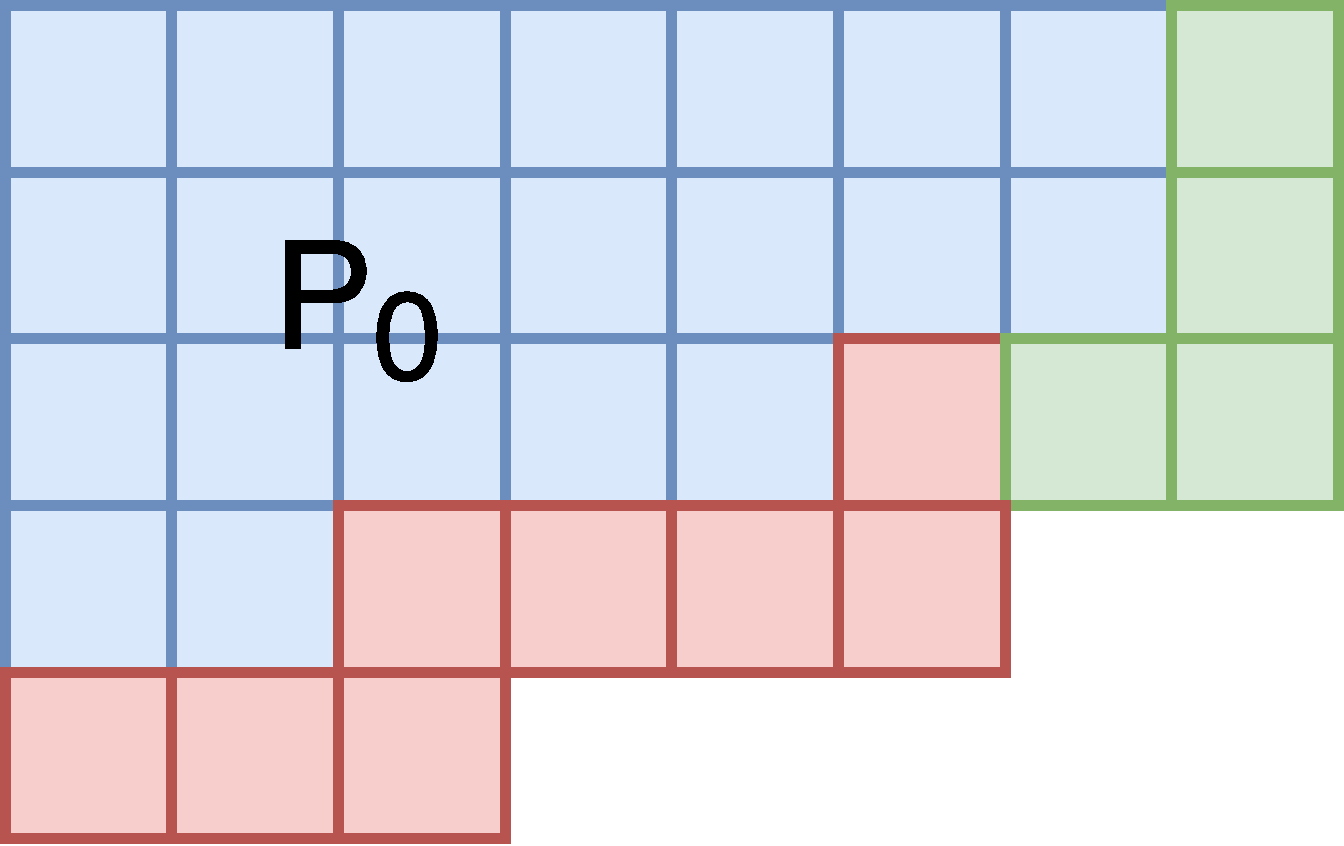
\includegraphics[width=\textwidth]{./PPT/Data_Syn_P0}
%\end{figure}
%\end{minipage}
%
%\begin{minipage}[b]{0.78\textwidth}
%\begin{figure}
%\flushright
%\includegraphics[width=0.615\textwidth]{./PPT/Data_Syn}
%\end{figure}
%\end{minipage}
%\begin{minipage}[b]{0.21\textwidth}
%\begin{figure}
%\flushright
%\includegraphics[width=0.78\textwidth]{./PPT/Data_Syn_P2}
%\end{figure}
%\end{minipage}
%
%\begin{minipage}[b]{0.25\textwidth}
%\begin{figure}
%\includegraphics[width=\textwidth]{./PPT/Data_Syn_P1}
%\end{figure}
%\end{minipage}
%\end{frame}
%
%\begin{frame}{Data Synchronization}
%
%\begin{minipage}{0.38\textwidth}
%\begin{figure}
%\flushleft
%\includegraphics[width=0.99\textwidth]{./Chapter-5/Figures/Work_flow}
%\end{figure}
%\end{minipage}
%\begin{minipage}{0.61\textwidth}
%Data are synchronized after every update:
%
%\begin{itemize}
%\item Pack up data to send them out together
%\item User defined MPI data structure for particles and buckets
%\item Overlap computing/pack/unpack with communication (with MPI non-blocking point to point communication)
%\item Avoid sending out useless data (e.g. neighbour information)
%\end{itemize}
%\end{minipage}
%
%\end{frame}

\begin{frame}{Load Balance check Interval}
The movement of particles and expansion of computational domain can lead to large load imbalance. We check the work load balance with an optimized interval and then redecompose the domain when necessary to restore work load balance.
\begin{figure}
\flushleft
\includegraphics[width=0.385\textwidth]{./Chapter-5/Figures/Work_flow}
\hfill
\includegraphics[width=0.435\textwidth]{./Chapter-5/Figures/int_bar}
\end{figure}
\end{frame}

%\begin{frame}{Dynamic Halo Domain}
%A lot of CPU time will be spent
%on computing associated with these stationary particles. The computational cost will be greatly reduced if the computational domain changes adaptively during simulation. 
%\begin{block}{Our strategy}
%  \begin{itemize}
%  \item {
%    An involvement flag to distinguish different states of involvement
%  }
%  \item {
%    A scan function to monitor the outermost layer of the domain
%  }
%  \item {
%    Shift pressure ghost particles into real particles when necessary
%  }
%  \end{itemize}
%\end{block}
%%
%\begin{figure}
%\flushleft
%\includegraphics[width=0.33\textwidth]{./PPT/t=66_msfrc}
%\hfill
%\includegraphics[width=0.33\textwidth]{./PPT/t=66_bctp}
%\hfill
%\includegraphics[width=0.33\textwidth]{./PPT/t=66_involved}
%\end{figure}
%\end{frame}

\begin{frame}{Dynamic Halo Domain}
\begin{minipage}{0.285 \textwidth}
\begin{figure}
\flushleft
\includegraphics[width=0.99\textwidth]{./PPT/t=66_msfrc}
\\
\flushleft
\includegraphics[width=0.99\textwidth]{./PPT/t=66_bctp}
\\
\flushleft
\includegraphics[width=0.99\textwidth]{./PPT/t=66_involved}
\end{figure}
\end{minipage}
\hfill
\begin{minipage}{0.34\textwidth}
\begin{figure}
\includegraphics[width=\textwidth]{./Chapter-5/Figures/Work_flow_adjust}
\end{figure}
\end{minipage}
\hfill
\begin{minipage}{0.355 \textwidth}
\begin{scriptsize}
\linespread{1.0}{
SWCH: switch pressure ghost particles to real. ADPP: add new pressure ghost particles. ADWP: add wall ghost particles. SCN: scann the outmost layer of the domain}
\end{scriptsize}
\center
\resizebox{0.99 \textwidth}{!}{
    \begin{tabular}{lrr}
    \hline
    Functions & Total time (s) & Called times\\
    	\hline
    UPME & 2954.8 & 201 \\
    UPP & 38.55 &  201 \\
    ADPP & 21.51 & 3 \\
    ADWP  & 8.88 & 3 \\
    SWCH & 0.08 &  2 \\
    SCN  & 7.72 & 201 \\
    \hline
  \end{tabular}}
\begin{figure}
\includegraphics[width=0.95\textwidth]  {./Chapter-5/Figures/adj_vs_no}
\end{figure}
\end{minipage}
\end{frame}

%\section{Scalability Test}
\begin{frame}{Scalability}
\begin{figure}
\flushleft
\includegraphics[width=0.31\textwidth]{./Chapter-5/Figures/strong_scale}
\hfill
\includegraphics[width=0.31\textwidth]{./Chapter-5/Figures/strong_scale_zoom}
\hfill
\includegraphics[width=0.31\textwidth]{./Chapter-5/Figures/weak_scale}
\caption{The left figure shows strong scalability tests result. middle figure is the zoomed view of first one. It is obviously shown that strong scalability is better when the problem size is larger. The right figure is weak scalability test results}
\label{fig:2cases_efficiency}
\end{figure}
%
\end{frame}
%----------------------------------------------------------------------------

%------------------------------------------------------------------
\section{Verification, Validation}
\begin{frame}{Verification and Validation}
\begin{figure}
\flushleft
\includegraphics[width=0.195\textwidth]{./PPT/shocktube}
\hfill
\includegraphics[width=0.195\textwidth]{./Chapter-6/Figures/conc_along_axis}
\hfill
\includegraphics[width=0.195\textwidth]{./Chapter-6/Figures/conc_cross}
\hfill
\includegraphics[width=0.195\textwidth]{./Chapter-6/Figures/velo_along_axis}
\hfill
\includegraphics[width=0.195\textwidth]{./Chapter-6/Figures/vel_cross}
\caption{Shock tube test and JPUE test verification: dimensionless velocity and concetration distribution along centraline and across the cross-section.}
\label{fig:JPUE_all}
\end{figure}
%
\begin{figure}
\flushleft
\includegraphics[width=0.17\textwidth]{./Chapter-6/Figures/radius_strong}
\hfill
\includegraphics[width=0.17\textwidth]{./Chapter-6/Figures/Temp}
\hfill
\includegraphics[width=0.17\textwidth]{./Chapter-6/Figures/density_strong}
\hfill
\includegraphics[width=0.40\textwidth]{./Chapter-6/Figures/msfrac}
\caption{Simulation of Pinatubo (Philippines, 15 June 1991) : integrated are profiles compared with existing mesh-based models}
\label{fig:JPUE_all}
\end{figure}
\end{frame}

\begin{frame}{Annimation of Pinatubo Eruption (SPH)}
Eruption condition, atmosphere, material propertities are mimic Pinatubo eruption (Philippines, 15 June 1991). \\
Eruption conditions: vent velocity is 275 $m\cdot s^{-1}$, vent gas mass fraction is 0.05, vent temperature is 1053 $K$, vent height is 1500 $km$, mass discharge rate is $1.5 \times 10^9 kg\cdot s^{-1}$. \\
%
\begin{minipage}{.32\linewidth}
\includemedia[
  label=vidA,
  width=0.99\linewidth,
  height=1.3\linewidth,
  activate=onclick,
  deactivate=onclick,
  addresource=./Movies/mssfrc_sml400.mp4,
  flashvars={source=./Movies/mssfrc_sml400.mp4 &loop=true}
  ]{}{VPlayer.swf}
\end{minipage}
\hfill
\begin{minipage}{.32\linewidth} 
  \includemedia[
  label=vidB,
  width=0.99\linewidth,
  height=1.3\linewidth,
  activate=onclick,
  deactivate=onclick,
  addresource=./Movies/cut_view_mssfrc_sml400.mp4,
  flashvars={source=./Movies/cut_view_mssfrc_sml400.mp4 &loop=true}]
  {}{VPlayer.swf}
\end{minipage}
\hfill  
\begin{minipage}{.32\linewidth} 
  \includemedia[
  label=vidC,
  width=0.99\linewidth,
  height=1.3\linewidth,
  activate=onclick,
  deactivate=onclick,
  addresource=./Movies/cut_view_Involved_sml400.mp4,
  flashvars={source=./Movies/cut_view_Involved_sml400.mp4 &loop=true}]
  {}{VPlayer.swf}
\end{minipage}
%  
  \mediabutton[
  mediacommand=vidA:playPause,
  mediacommand=vidB:playPause,
  mediacommand=vidC:playPause,
]{\fbox{Play/Pause}}
%
\end{frame}

\begin{frame}{Short Period Eruption}
\begin{minipage}{.49\linewidth} 
  \includemedia[
  label=vidB,
  width=0.99\linewidth,
  height=1.3\linewidth,
  activate=onclick,
  deactivate=onclick,
  addresource=./Movies/sml400-100s-massfrc.mp4,
  flashvars={source=./sml400-100s-massfrc.mp4 &loop=true}]
  {}{VPlayer.swf}
\end{minipage}
\hfill  
\begin{minipage}{.49\linewidth} 
  \includemedia[
  label=vidC,
  width=0.99\linewidth,
  height=1.3\linewidth,
  activate=onclick,
  deactivate=onclick,
  addresource=./Movies/sml400-300s-massfrc.mp4,
  flashvars={source=./Movies/sml400-300s-massfrc.mp4 &loop=true}]
  {}{VPlayer.swf}
\end{minipage}
%  
  \mediabutton[
  mediacommand=vidA:playPause,
  mediacommand=vidB:playPause,
  mediacommand=vidC:playPause,
]{\fbox{Play/Pause}}
%
\end{frame}

\begin{frame}{GSPH and RSPH}
\begin{minipage}{.49\linewidth} 
  \includemedia[
  label=vidB,
  width=0.99\linewidth,
  height=1.3\linewidth,
  activate=onclick,
  deactivate=onclick,
  addresource=./Movies/GSPH_mssfrc_640_HSV.mp4,
  flashvars={source=./Movies/GSPH_mssfrc_640_HSV.mp4  &loop=true}]
  {}{VPlayer.swf}
\end{minipage}
\hfill  
\begin{minipage}{.49\linewidth} 
  \includemedia[
  label=vidC,
  width=0.99\linewidth,
  height=1.3\linewidth,
  activate=onclick,
  deactivate=onclick,
  addresource=./Movies/RSPH_mssfrc_HSV.mp4,
  flashvars={source=./Movies/RSPH_mssfrc_HSV.mp4 &loop=true}]
  {}{VPlayer.swf}
\end{minipage}
%  
  \mediabutton[
  mediacommand=vidA:playPause,
  mediacommand=vidB:playPause,
  mediacommand=vidC:playPause,
]{\fbox{Play/Pause}}
%
\end{frame}

\section{Plume-SPH + VATDs}
\begin{frame}{Initial Ash Cloud}
\begin{minipage}{.67\textwidth}
\textbf{Create Initial condition based on 1D model}
\begin{itemize}
\item 1D model predict $H_{max}$, $H_{width}$ and $R_{width}$.
\item\begin{equation}
H=H_{max} - 0.5 H_{width}*P+H_{width}R
\label{eq:Poisson-plume-shape}
\end{equation}
$P$: random number from a Poisson
distribution of unit mean \\ 
$R$: a uniformly distributed random number between 0 and 1
\item Distribute ash horizontally uniformally according to $R_{width}$
\item Generate the initial ash cloud.
\end{itemize}
\end{minipage}
\noindent
\begin{minipage}{.32\textwidth}
\includegraphics[width=0.99\textwidth]{./PPT/Creat_initial_Ash}
\end{minipage} % This must go next to 
%
\end{frame}

\begin{frame}{Vertical ash distribution}
\begin{figure}
    \centering
    \begin{minipage}{.30 \textwidth}
        \centering
        \includegraphics[width=0.90 \textwidth]{Chapter-7/Figures/Plume-SPH-ParticleDis-NoTrucation-z}
    \end{minipage}%
    \begin{minipage}{.30 \textwidth}
        \centering
        \includegraphics[width=0.90 \textwidth]{Chapter-7/Figures/Plume-SPH-ParticleDis-z}
    \end{minipage}%
    \begin{minipage}{.30 \textwidth}
        \centering
        \includegraphics[width=0.90 \textwidth]{Chapter-7/Figures/Possion-Hmax40k-ParticleDis-z}
    \end{minipage}% 
%    \caption{Particle distribution of initial ash cloud in vertical direction. The picture to the left is corresponding to initial ash cloud obtained from Plume-SPH output. The second picture is corresponding to ash distribution truncated by a elevation threshold of $15000 m$. Third picture is corresponding to Poisson distribution with maximum height based on bent simulation. Another parameter, the vertical spread, in the expression of Poisson plume shape is $6662 m$. The picture to the right is corresponding to Suzuki distribution with maximum height based on bent simulation. Another parameter in Suzuki distribution, the shape factor, is $4$. The $x$ axis is the percentage of particle number for Plume-SPH and Poisson, is the percentage of erupted material mass percentage for Suzuki.}
\end{figure}

\begin{figure}
\center
\includegraphics[width=0.60 \textwidth]{Chapter-7/Figures/Restart-PUFF} 
%    \caption{Mimic successive eruption with intermittent pulsing releasing of ash particles. $t_I$ is the period of pulsing release. $t_I$ equals to physical time of plume simulation.}
\end{figure}

\end{frame}

\begin{frame}{Ash transportation}
\begin{figure}[!htb]
    \centering
    \begin{minipage}{.295\textwidth}
        \centering
        \includegraphics[width=0.99 \textwidth]{./Chapter-7/Figures/bent-23hr-ash}
    \end{minipage}%
    \begin{minipage}{.295\textwidth}
        \centering
        \includegraphics[width=0.99 \textwidth]{./Chapter-7/Figures/SPH-Plume-23hr-ash}
    \end{minipage}%
    \begin{minipage}{.295\textwidth}
        \centering
        \includegraphics[width=0.99 \textwidth]{./Chapter-7/Figures/OB-ash-23hr-ash}
    \end{minipage}% 
    \\
        \begin{minipage}{.295\textwidth}
        \centering
        \includegraphics[width=0.99 \textwidth]{./Chapter-7/Figures/bent-31hr-ash}
    \end{minipage}%
    \begin{minipage}{.295\textwidth}
        \centering
        \includegraphics[width=0.99 \textwidth]{./Chapter-7/Figures/SPH-Plume-31hr-ash}
    \end{minipage}%
    \begin{minipage}{.295\textwidth}
        \centering
        \includegraphics[width=0.99 \textwidth]{./Chapter-7/Figures/OB-ash-31hr-ash}
    \end{minipage}% 
    \\
        \begin{minipage}{.295\textwidth}
        \centering
        \includegraphics[width=0.99 \textwidth]{./Chapter-7/Figures/bent-55hr-ash}
    \end{minipage}%
    \begin{minipage}{.295\textwidth}
        \centering
        \includegraphics[width=0.99 \textwidth]{./Chapter-7/Figures/SPH-Plume-55hr-ash}
    \end{minipage}%
    \begin{minipage}{.295\textwidth}
        \centering
        \includegraphics[width=0.99 \textwidth]{./Chapter-7/Figures/OB-ash-55hr-ash}
    \end{minipage}% 
    \caption{Taking the output of the SPH plume model as initial condition to forecast volcanic ash transportation.}
    \label{fig:Plume-SPH-Pinatubo-SO2-cloud}
\end{figure}
\end{frame}

%----------------------------------------------------------------------------
\section{Future Work}
\begin{frame} {Future work}
\begin{figure}
	\includegraphics[width=0.5\textwidth]{./PPT/Future-Work}
\end{figure}
\end{frame}
%
\begin{frame}{}
\center
\huge{
Thanks to \\}
\Large
{
Dr. Patra \\
Dr. Bursik, Dr. Pitman, Dr. Bauman \\
Dr. Jones, Dinesh, Hossein, Ramona, Topher \\
Prashant, Lekha, Qingyuan, Abhishek, Ali, Renette, Miaoda ...\\
My family \\
}
\end{frame}


%% All of the following is optional and typically not needed. 
%\appendix
%\section<presentation>*{\appendixname}
%\subsection<presentation>*{For Further Reading}
%
%\begin{frame}[allowframebreaks]
%  \frametitle<presentation>{For Further Reading}
%    
%  \begin{thebibliography}{10}
%    
%  \beamertemplatebookbibitems
%  % Start with overview books.
%
%  \bibitem{Author1990}
%    A.~Author.
%    \newblock {\em Handbook of Everything}.
%    \newblock Some Press, 1990.
% 
%    
%  \beamertemplatearticlebibitems
%  % Followed by interesting articles. Keep the list short. 
%
%  \bibitem{Someone2000}
%    S.~Someone.
%    \newblock On this and that.
%    \newblock {\em Journal of This and That}, 2(1):50--100,
%    2000.
%  \end{thebibliography}
%\end{frame}

\end{document}


